\documentclass[]{book}
\usepackage{lmodern}
\usepackage{amssymb,amsmath}
\usepackage{ifxetex,ifluatex}
\usepackage{fixltx2e} % provides \textsubscript
\ifnum 0\ifxetex 1\fi\ifluatex 1\fi=0 % if pdftex
  \usepackage[T1]{fontenc}
  \usepackage[utf8]{inputenc}
  \usepackage{eurosym}
\else % if luatex or xelatex
  \ifxetex
    \usepackage{mathspec}
  \else
    \usepackage{fontspec}
  \fi
  \defaultfontfeatures{Ligatures=TeX,Scale=MatchLowercase}
  \newcommand{\euro}{€}
\fi
% use upquote if available, for straight quotes in verbatim environments
\IfFileExists{upquote.sty}{\usepackage{upquote}}{}
% use microtype if available
\IfFileExists{microtype.sty}{%
\usepackage{microtype}
\UseMicrotypeSet[protrusion]{basicmath} % disable protrusion for tt fonts
}{}
\usepackage[margin=1in]{geometry}
\usepackage{hyperref}
\hypersetup{unicode=true,
            pdftitle={FAQ Laboratori de Fonaments de Programació},
            pdfauthor={Jordi Blasco Planesas},
            pdfborder={0 0 0},
            breaklinks=true}
\urlstyle{same}  % don't use monospace font for urls
\usepackage{natbib}
\bibliographystyle{apalike}
\usepackage{color}
\usepackage{fancyvrb}
\newcommand{\VerbBar}{|}
\newcommand{\VERB}{\Verb[commandchars=\\\{\}]}
\DefineVerbatimEnvironment{Highlighting}{Verbatim}{commandchars=\\\{\}}
% Add ',fontsize=\small' for more characters per line
\usepackage{framed}
\definecolor{shadecolor}{RGB}{248,248,248}
\newenvironment{Shaded}{\begin{snugshade}}{\end{snugshade}}
\newcommand{\KeywordTok}[1]{\textcolor[rgb]{0.13,0.29,0.53}{\textbf{#1}}}
\newcommand{\DataTypeTok}[1]{\textcolor[rgb]{0.13,0.29,0.53}{#1}}
\newcommand{\DecValTok}[1]{\textcolor[rgb]{0.00,0.00,0.81}{#1}}
\newcommand{\BaseNTok}[1]{\textcolor[rgb]{0.00,0.00,0.81}{#1}}
\newcommand{\FloatTok}[1]{\textcolor[rgb]{0.00,0.00,0.81}{#1}}
\newcommand{\ConstantTok}[1]{\textcolor[rgb]{0.00,0.00,0.00}{#1}}
\newcommand{\CharTok}[1]{\textcolor[rgb]{0.31,0.60,0.02}{#1}}
\newcommand{\SpecialCharTok}[1]{\textcolor[rgb]{0.00,0.00,0.00}{#1}}
\newcommand{\StringTok}[1]{\textcolor[rgb]{0.31,0.60,0.02}{#1}}
\newcommand{\VerbatimStringTok}[1]{\textcolor[rgb]{0.31,0.60,0.02}{#1}}
\newcommand{\SpecialStringTok}[1]{\textcolor[rgb]{0.31,0.60,0.02}{#1}}
\newcommand{\ImportTok}[1]{#1}
\newcommand{\CommentTok}[1]{\textcolor[rgb]{0.56,0.35,0.01}{\textit{#1}}}
\newcommand{\DocumentationTok}[1]{\textcolor[rgb]{0.56,0.35,0.01}{\textbf{\textit{#1}}}}
\newcommand{\AnnotationTok}[1]{\textcolor[rgb]{0.56,0.35,0.01}{\textbf{\textit{#1}}}}
\newcommand{\CommentVarTok}[1]{\textcolor[rgb]{0.56,0.35,0.01}{\textbf{\textit{#1}}}}
\newcommand{\OtherTok}[1]{\textcolor[rgb]{0.56,0.35,0.01}{#1}}
\newcommand{\FunctionTok}[1]{\textcolor[rgb]{0.00,0.00,0.00}{#1}}
\newcommand{\VariableTok}[1]{\textcolor[rgb]{0.00,0.00,0.00}{#1}}
\newcommand{\ControlFlowTok}[1]{\textcolor[rgb]{0.13,0.29,0.53}{\textbf{#1}}}
\newcommand{\OperatorTok}[1]{\textcolor[rgb]{0.81,0.36,0.00}{\textbf{#1}}}
\newcommand{\BuiltInTok}[1]{#1}
\newcommand{\ExtensionTok}[1]{#1}
\newcommand{\PreprocessorTok}[1]{\textcolor[rgb]{0.56,0.35,0.01}{\textit{#1}}}
\newcommand{\AttributeTok}[1]{\textcolor[rgb]{0.77,0.63,0.00}{#1}}
\newcommand{\RegionMarkerTok}[1]{#1}
\newcommand{\InformationTok}[1]{\textcolor[rgb]{0.56,0.35,0.01}{\textbf{\textit{#1}}}}
\newcommand{\WarningTok}[1]{\textcolor[rgb]{0.56,0.35,0.01}{\textbf{\textit{#1}}}}
\newcommand{\AlertTok}[1]{\textcolor[rgb]{0.94,0.16,0.16}{#1}}
\newcommand{\ErrorTok}[1]{\textcolor[rgb]{0.64,0.00,0.00}{\textbf{#1}}}
\newcommand{\NormalTok}[1]{#1}
\usepackage{longtable,booktabs}
\usepackage{graphicx,grffile}
\makeatletter
\def\maxwidth{\ifdim\Gin@nat@width>\linewidth\linewidth\else\Gin@nat@width\fi}
\def\maxheight{\ifdim\Gin@nat@height>\textheight\textheight\else\Gin@nat@height\fi}
\makeatother
% Scale images if necessary, so that they will not overflow the page
% margins by default, and it is still possible to overwrite the defaults
% using explicit options in \includegraphics[width, height, ...]{}
\setkeys{Gin}{width=\maxwidth,height=\maxheight,keepaspectratio}
\IfFileExists{parskip.sty}{%
\usepackage{parskip}
}{% else
\setlength{\parindent}{0pt}
\setlength{\parskip}{6pt plus 2pt minus 1pt}
}
\setlength{\emergencystretch}{3em}  % prevent overfull lines
\providecommand{\tightlist}{%
  \setlength{\itemsep}{0pt}\setlength{\parskip}{0pt}}
\setcounter{secnumdepth}{5}
% Redefines (sub)paragraphs to behave more like sections
\ifx\paragraph\undefined\else
\let\oldparagraph\paragraph
\renewcommand{\paragraph}[1]{\oldparagraph{#1}\mbox{}}
\fi
\ifx\subparagraph\undefined\else
\let\oldsubparagraph\subparagraph
\renewcommand{\subparagraph}[1]{\oldsubparagraph{#1}\mbox{}}
\fi

%%% Use protect on footnotes to avoid problems with footnotes in titles
\let\rmarkdownfootnote\footnote%
\def\footnote{\protect\rmarkdownfootnote}

%%% Change title format to be more compact
\usepackage{titling}

% Create subtitle command for use in maketitle
\providecommand{\subtitle}[1]{
  \posttitle{
    \begin{center}\large#1\end{center}
    }
}

\setlength{\droptitle}{-2em}

  \title{FAQ Laboratori de Fonaments de Programació}
    \pretitle{\vspace{\droptitle}\centering\huge}
  \posttitle{\par}
    \author{Jordi Blasco Planesas}
    \preauthor{\centering\large\emph}
  \postauthor{\par}
      \predate{\centering\large\emph}
  \postdate{\par}
    \date{2020-03-28}

\usepackage{booktabs}
\usepackage{amsthm}
\makeatletter
\def\thm@space@setup{%
  \thm@preskip=8pt plus 2pt minus 4pt
  \thm@postskip=\thm@preskip
}
\makeatother

\begin{document}
\maketitle

{
\setcounter{tocdepth}{1}
\tableofcontents
}
\chapter*{Introducció}\label{introduccio}
\addcontentsline{toc}{chapter}{Introducció}

El present recurs és un recopilatori de qüestions plantejades al
\textbf{Laboratori de Fonaments de Programació} durant els últims
semestres.

Les \textbf{FAQ} poden donar resposta a dubtes i errors habituals en el
moment d'iniciar-nos en el món de la programació. També es poden
utilitzar com a material complementari a la teoria explicada a la
\textbf{xWiki} de \textbf{Fonaments de Programació}.

La lectura de les FAQ no cal realitzar-la seqüencialment: cada apartat
respon a una consulta o conjunt de consultes, sense relació necessària
entre elles.

El fil conductor són les \textbf{PAC} : les diferents respostes donades
al \textbf{Laboratori de Fonaments de Programació} s'han agrupat en PAC
segons el moment en que es van produïr. Això no significa que una
resposta d'una PAC anterior o posterior a la que estiguem tractant, no
ens pugui ser d'utilitat.

Donada aquesta independència de contingut és recomanable utilitzar el
cercador del portal: per exemple, si volem cercar consultes on s'hagi
tractat \texttt{strlen}, simplement posem aquesta comanda al cercador i
obtindrem la relació d'entrades que la contenen.

És possible descarregar una versió en PDF/EPUB de totes les FAQ, des del
botó de descàrrega de la part superior.

La documentació utilitza les següents icones per referenciar els blocs:

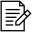
\includegraphics{./img/alg.png} Indica que el codi mostrat està en
\textbf{llenguatge algorísmic}.


\includegraphics{./img/c.png} Indica que el codi mostrat està en
\textbf{llenguatge C}.

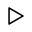
\includegraphics{./img/play.png} Mostra l'execució d'un programa en
\textbf{llenguatge C}.

\chapter{PAC01}\label{pac01}

\section{Llenguatge algorísmic}\label{llenguatge-algorismic}

El llenguatge algorísmic l'hem d'entendre com una aproximació al món
real, el qual utilitza unes normes definides per nosaltres mateixos. En
aquest punt encara no parlem de programes escrits en \textbf{C}, en
\textbf{Java}, en \textbf{Python} o en \textbf{PHP}, per dir alguns
llenguatges de programació.

Per exemple, en el llenguatge algorísmic que utilitzem a l'assignatura
definim un bloc de variables de la següent forma:

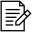
\includegraphics{./img/alg.png}

\begin{verbatim}
var
    edat: integer;
    pes: real;
end var
\end{verbatim}

Que es tracti d'un llenguatge més proper al món real no significa que no
s'hagin de complir unes determinades regles. Com es pot veure en aquest
exemple, una d'aquestes regles és que quan definim variables ho precedim
amb \texttt{var} i ho finalitzem amb \texttt{end\ var}.

Hem decidit utilitzar aquesta forma de llenguatge algorísmic, tot i que
també ho podríem haver plantejat de la següent forma :

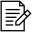
\includegraphics{./img/alg.png}

\begin{verbatim}
variable
    enter edat
    decimal pes
fvariable
\end{verbatim}

Remarcar que aquest segon exemple \textbf{és incorrecte}, no segueix la
nomenclatura del llenguatge algorísmic definit a l'assignatura. El
correcte és el primer exemple.

El llenguatge algorísmic és com fer una aproximació formal a la
realitat, no és un llenguatge de programació en sí com és \textbf{C},
\textbf{Java} o similars. Per tant no és un llenguatge que es pugui
compilar i executar amb l'IDE utilitzat a l'assignatura, el qual està
preparat únicament per interpretar i executar codi programat en
llenguatge C.

Ara bé la gran pregunta: i per què és necessari primer dissenyar
l'algorisme, si puc directament programar-ho en C?

Un algorisme ens permet dissenyar un programa sense tenir presents les
particularitats de cada llenguatge de programació. Aquesta aproximació
formal a la realitat dels algorismes ens faciliten poder fer
posteriorment una traducció ràpida a qualsevol llenguatge de programació
simplement coneixent les equivalències corresponents. Per exemple, el
primer cas si el programem en C equival a:


\includegraphics{./img/c.png}

\begin{Shaded}
\begin{Highlighting}[]
\DataTypeTok{int}\NormalTok{ edat;}
\DataTypeTok{float}\NormalTok{ pes;}
\end{Highlighting}
\end{Shaded}

El codi en C no el podem canviar, ja que si en comptes de posar int
utilitzem enter, el compilador de C no comprèn el mot i ens donarà un
error de codi.

Si mai hem programat és normal que aquest plantejament sobti al
principi, però és important que poc a poc es vagi veient les diferències
entre llenguatge algorísmic i llenguatge C.

\section{Llenguatge algorísmic vs llenguatge
C}\label{llenguatge-algorismic-vs-llenguatge-c}

En general:

\begin{itemize}
\tightlist
\item
  \textbf{Llenguatge algorísmic}: proper al llenguatge natural, es
  tracta d'una convenció que adoptem nosaltres mateixos per definir el
  un programa formalment. Els algorismes tenen una sèrie de normes i
  sentències que nosaltres definim (\textbf{Nomenclàtor}), però que no
  són de cap forma interpretables per un ordinador. Per tant un
  algorisme \textbf{no pot ser compilat ni executat}.
\item
  \textbf{Llenguatge C}: es tracta d'un llenguatge de programació que sí
  comprèn un ordinador. Això significa que únicament podem utilitzar les
  seves comandes i les seves normes per tal que el codi pugui ser
  compilat i executat sense problemes.
\end{itemize}

El llenguatge algorísmic és un pseudocodi que ens ajuda a definir com
funciona un programa. No està lligat a cap llenguatge de programació,
amb el que les accions que realitzarà, la forma de definir variables,
etc. és genèrica. Funcions com \texttt{writeString()},
\texttt{readInteger()} o \texttt{writeChar()} formen part del llenguatge
algorísmic: indiquen una acció genèrica a realitzar, com és escriure una
cadena de caracters, llegir un enter o escriure un caràcter. Quan es
vulgui codificar aquest algorisme en un llenguatge de programació
concret com és C, només caldrà saber les comandes pròpies de C que ens
permeten implementar l'algorisme.

La programació en C funciona exclusivament amb la sintaxi definida per
aquest llenguatge de programació. Instruccions com \texttt{scanf()} i
\texttt{printf()} són pròpies de C.

A mode d'exemple:

\textbf{Algorisme}: volem introduïr la lectura de la llum de casa
nostra; una possible implementació és:

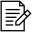
\includegraphics{./img/alg.png}

\begin{verbatim}
algorithm lecturaLlum
    var
        lecturaMensual: integer;
    end var

    writeString("Introdueix la lectura mensual de la llum (kWh): ");
    lecturaMensual := readInteger();
end algorithm
\end{verbatim}

\textbf{Llenguatge C}: en aquest llenguatge no existeixen les funcions
algorísmiques \texttt{writeString()} ni \texttt{readInteger()}, però en
canvi sí que tenim vàries funcions pròpies de C que ens permeten llegir
un valor per teclat i assignar-lo a una variable d'entorn. Per tant, les
accions algorísmiques anteriors correspondran a la següent codificació
en C:


\includegraphics{./img/c.png}

\begin{Shaded}
\begin{Highlighting}[]
\PreprocessorTok{#include }\ImportTok{<stdio.h>}

\DataTypeTok{int}\NormalTok{ main(}\DataTypeTok{int}\NormalTok{ argc, }\DataTypeTok{char}\NormalTok{ **argv) \{ }
    \DataTypeTok{int}\NormalTok{ lecturaMensual;}

\NormalTok{    printf(}\StringTok{"Introdueix la lectura mensual de la llum (kWh): "}\NormalTok{);}
\NormalTok{    scanf(}\StringTok{"%d"}\NormalTok{, &lecturaMensual);}
    \ControlFlowTok{return} \DecValTok{0}\NormalTok{;}
\NormalTok{\}}
\end{Highlighting}
\end{Shaded}

És molt important que es vegi clarament què és un algorisme i què és un
programa en C.

\section{Equivalències llenguatge algorísmic vs llenguatge
C}\label{equivalencies-llenguatge-algorismic-vs-llenguatge-c}

A continuació s'indiquen algunes de les equivalències existents entre
llenguatge algorísmic i el llenguatge de programació C:

\begin{longtable}[]{@{}lcc@{}}
\toprule
& Llenguatge algorísmic & Llenguatge C\tabularnewline
\midrule
\endhead
Segueix unes normes? & sí & sí\tabularnewline
Es pot compilar? & no & sí\tabularnewline
Es pot executar? & no & sí\tabularnewline
Assignació de valors a variables & \texttt{:=} &
\texttt{=}\tabularnewline
Tipus booleà & \texttt{boolean} & \texttt{bool}\tabularnewline
Tipus enter & \texttt{integer} & \texttt{int}\tabularnewline
Tipus decimal & \texttt{real} & \texttt{float}\tabularnewline
Tipus caràcter & \texttt{char} & \texttt{char}\tabularnewline
Operador igual & \texttt{=} & \texttt{==}\tabularnewline
Operador diferent & \texttt{≠} & \texttt{!=}\tabularnewline
Operador major & \texttt{\textgreater{}} &
\texttt{\textgreater{}}\tabularnewline
Operador major o igual & \texttt{≥} &
\texttt{\textgreater{}=}\tabularnewline
Operador menor & \texttt{\textless{}} &
\texttt{\textless{}}\tabularnewline
Operador menor o igual & \texttt{≤} &
\texttt{\textless{}=}\tabularnewline
Operador lògic de conjunció & \texttt{and} &
\texttt{\&\&}\tabularnewline
Operador lògic de disjunció & \texttt{or} &
\texttt{\textbar{}\textbar{}}\tabularnewline
Operador lògic de negació & \texttt{not} & \texttt{!}\tabularnewline
\bottomrule
\end{longtable}

\section{Impressió de valors
incorrecta}\label{impressio-de-valors-incorrecta}

Quan es mostra per pantalla el contingut d'alguna variable amb
\texttt{printf()}, és important eliminar el prefix \texttt{\&} de la
variable. Per exemple, si no ho fem tenim que:


\includegraphics{./img/c.png}

\begin{Shaded}
\begin{Highlighting}[]
\PreprocessorTok{#include }\ImportTok{<stdio.h>}

\DataTypeTok{int}\NormalTok{ main(}\DataTypeTok{int}\NormalTok{ argc, }\DataTypeTok{char}\NormalTok{ **argv)\{}

    \DataTypeTok{int}\NormalTok{ idAvio;}

\NormalTok{    printf(}\StringTok{"Introdueix l'identificador d'avió : "}\NormalTok{);}
\NormalTok{    scanf(}\StringTok{"%d"}\NormalTok{, &idAvio);}
    
\NormalTok{    printf(}\StringTok{">> Has escollit l'avió amb id %d }\SpecialCharTok{\textbackslash{}n}\StringTok{"}\NormalTok{, &idAvio);}

    \ControlFlowTok{return} \DecValTok{0}\NormalTok{;}
\NormalTok{\}}
\end{Highlighting}
\end{Shaded}

El resultat de l'execució és:


\includegraphics{./img/c.png}

\begin{Shaded}
\begin{Highlighting}[]
\NormalTok{Introdueix l'identificador d'avió : }\DecValTok{9}
\NormalTok{>> Has escollit l'avió amb id -}\DecValTok{1078693464}
\end{Highlighting}
\end{Shaded}

Per quin motiu obtenim el valor estrany en l'identificador d'avió? Quan
fem referència a \texttt{\&idAvio} estem obtenint realment la posició de
memòria on resideix la variable \texttt{idAvio}, no pas el valor de la
variable. Per obtenir el seu valor cal eliminar de dins
\texttt{printf()} el prefix \texttt{\&} de la variable \texttt{idAvio}:


\includegraphics{./img/c.png}

\begin{Shaded}
\begin{Highlighting}[]
\PreprocessorTok{#include }\ImportTok{<stdio.h>}

\DataTypeTok{int}\NormalTok{ main(}\DataTypeTok{int}\NormalTok{ argc, }\DataTypeTok{char}\NormalTok{ **argv)\{}

    \DataTypeTok{int}\NormalTok{ idAvio;}

\NormalTok{    printf(}\StringTok{"Introdueix l'identificador d'avió : "}\NormalTok{);}
\NormalTok{    scanf(}\StringTok{"%d"}\NormalTok{, &idAvio);}
    
\NormalTok{    printf(}\StringTok{">> Has escollit l'avió amb id %d }\SpecialCharTok{\textbackslash{}n}\StringTok{"}\NormalTok{, idAvio);}

    \ControlFlowTok{return} \DecValTok{0}\NormalTok{;}
\NormalTok{\}}
\end{Highlighting}
\end{Shaded}

La sortida generada ara sí és correcta:

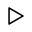
\includegraphics{./img/play.png}

\begin{Shaded}
\begin{Highlighting}[]
\NormalTok{Introdueix l'identificador d'avió : }\DecValTok{9}
\NormalTok{>> Has escollit l'avió amb id }\DecValTok{9} 
\end{Highlighting}
\end{Shaded}

\section{Com definir un enumeratiu}\label{com-definir-un-enumeratiu}

La definició d'un tipus enumeratiu en llenguatge algorísmic es fa de la
següent forma:

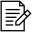
\includegraphics{./img/alg.png}

\begin{verbatim}
type
    typeName = {VALUE1, VALUE2, VALUE3, ... , VALUEn};
end type
\end{verbatim}

Els elements \texttt{VALUE1}, \texttt{VALUE2}, \texttt{VALUE3}\ldots{}
acaben sent constants, i el valor que de cadascun és:

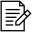
\includegraphics{./img/alg.png}

\begin{verbatim}
VALUE1 = 0
VALUE2 = 1
VALUE3 = 2 
{ ... }
VALUEn = n-1
\end{verbatim}

Posteriorment no és possible fer un canvi de valor d'aquests elements de
tipus enumeratiu.

\section{Com utilitzar un enumeratiu}\label{com-utilitzar-un-enumeratiu}

Una enumeració és una assignació d'un valor enter a la sèrie d'elements
que s'hi ha definit, començant pel 0 i incrementant-se en 1 en cada
element.

Per exemple, podem tenir la següent definició:


\includegraphics{./img/c.png}

\begin{Shaded}
\begin{Highlighting}[]
\KeywordTok{typedef} \KeywordTok{enum}\NormalTok{ \{MALE, FEMALE\} tGender;}
\end{Highlighting}
\end{Shaded}

Això significa que \texttt{MALE\ ==\ 0} i \texttt{FEMALE\ ==\ 1}. Si
l'ordre de la definició l'haguessis fet al revés,
\texttt{\{FEMALE,\ MALE\}}, tindríem que \texttt{FEMALE\ ==\ 0} i
\texttt{MALE\ ==\ 1}.

Una possible forma d'utilitzar els enumeratius es llegir un enter i
comparar-lo amb l'element corresponent definit dins de l'\texttt{enum},
per tal de realitzar una acció o una altra. Una possible implementació
en llenguatge C seria:


\includegraphics{./img/c.png}

\begin{Shaded}
\begin{Highlighting}[]
\PreprocessorTok{#include }\ImportTok{<stdio.h>}

\KeywordTok{typedef} \KeywordTok{enum}\NormalTok{ \{MALE, FEMALE\} tGender;}

\DataTypeTok{int}\NormalTok{ main(}\DataTypeTok{int}\NormalTok{ argc, }\DataTypeTok{char}\NormalTok{ **argv) \{}
\NormalTok{   tGender gender;}

\NormalTok{   printf(}\StringTok{"Type patient gender: 0 for MALE, 1 for FEMALE}\SpecialCharTok{\textbackslash{}n}\StringTok{"}\NormalTok{);}
\NormalTok{   scanf(}\StringTok{"%u"}\NormalTok{, &gender);}

   \ControlFlowTok{if}\NormalTok{ (gender == MALE) \{}
\NormalTok{      printf(}\StringTok{"Patient gender MALE}\SpecialCharTok{\textbackslash{}n}\StringTok{"}\NormalTok{);}
\NormalTok{   \} }\ControlFlowTok{else}\NormalTok{ \{}
      \ControlFlowTok{if}\NormalTok{ (gender == FEMALE) \{}
\NormalTok{         printf(}\StringTok{"Patient gender FEMALE}\SpecialCharTok{\textbackslash{}n}\StringTok{"}\NormalTok{);}
\NormalTok{      \} }\ControlFlowTok{else}\NormalTok{ \{}
\NormalTok{         printf(}\StringTok{"Incorrect option}\SpecialCharTok{\textbackslash{}n}\StringTok{"}\NormalTok{);}
\NormalTok{      \}}
\NormalTok{   \}}
   \ControlFlowTok{return} \DecValTok{0}\NormalTok{;}
\NormalTok{\}}
\end{Highlighting}
\end{Shaded}

\section{Especificador d'un
enumeratiu}\label{especificador-dun-enumeratiu}

Els enumeratius en llenguatge C, \texttt{enum}, utilitzen
l'especificador \texttt{\%u} independentment del tipus que s'hagi
definit per l'enumeratiu.

Exemple:


\includegraphics{./img/c.png}

\begin{Shaded}
\begin{Highlighting}[]
\PreprocessorTok{#include }\ImportTok{<stdio.h>}

\KeywordTok{typedef} \KeywordTok{enum}\NormalTok{ \{PRIVAT, PUBLIC\} tTransport;}

\DataTypeTok{int}\NormalTok{ main(}\DataTypeTok{int}\NormalTok{ argc, }\DataTypeTok{char}\NormalTok{ **argv) \{}
\NormalTok{    tTransport tipusTransport;}

\NormalTok{    printf(}\StringTok{"Amb quin tipus de transport et desplaces a la feina (0=privat, 1=públic) ? : "}\NormalTok{);}
\NormalTok{    scanf(}\StringTok{"%u"}\NormalTok{, &tipusTransport);}
\NormalTok{    printf(}\StringTok{"Et desplaces a la feina amb transport (0=privat, 1=públic) : "}\NormalTok{);}
\NormalTok{    printf(}\StringTok{"%u}\SpecialCharTok{\textbackslash{}n}\StringTok{"}\NormalTok{, tipusTransport);}
    \ControlFlowTok{return} \DecValTok{0}\NormalTok{;}
\NormalTok{\}}
\end{Highlighting}
\end{Shaded}

\section{Lectura de caràcters en C}\label{lectura-de-caracters-en-c}

En el llenguatge C la lectura d'un \texttt{char} pot comportar-se de
forma inadequada si prèviament el buffer d'entrada conté algun caràcter
previ.

Imaginem que volem crear un programa molt senzill que donat un número de
DNI i la seva lletra, ens concateni els dos valors i ho mostri per
pantalla. Una possible forma d'implementar aquest programa en C seria:


\includegraphics{./img/c.png}

\begin{Shaded}
\begin{Highlighting}[]
\PreprocessorTok{#include }\ImportTok{<stdio.h>}

\DataTypeTok{int}\NormalTok{ main(}\DataTypeTok{int}\NormalTok{ argc, }\DataTypeTok{char}\NormalTok{ **argv) \{}

    \DataTypeTok{int}\NormalTok{ dniNum;    }\CommentTok{/* número del DNI */}
    \DataTypeTok{char}\NormalTok{ dniChar;  }\CommentTok{/* lletra del DNI */}

\NormalTok{    printf(}\StringTok{"Introdueix el número del DNI: "}\NormalTok{);}
\NormalTok{    scanf(}\StringTok{"%d"}\NormalTok{, &dniNum);}
\NormalTok{    printf(}\StringTok{"Introdueix la lletra del DNI: "}\NormalTok{);}
\NormalTok{    scanf(}\StringTok{"%c"}\NormalTok{, &dniChar);}

\NormalTok{    printf(}\StringTok{"}\SpecialCharTok{\textbackslash{}n}\StringTok{El DNI introduit és: %d-%c}\SpecialCharTok{\textbackslash{}n}\StringTok{"}\NormalTok{, dniNum, dniChar);}
    \ControlFlowTok{return} \DecValTok{0}\NormalTok{;}
\NormalTok{\}}
\end{Highlighting}
\end{Shaded}

Què passa si executem aquest codi? Que veiem que es comporta de forma
incorrecta, ja que no ens arriba a demanar la lletra del DNI, mostrant
directament el resultat:

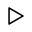
\includegraphics{./img/play.png}

\begin{Shaded}
\begin{Highlighting}[]
\NormalTok{Introdueix el número del DNI: }\DecValTok{12345678}
\NormalTok{Introdueix la lletra del DNI:}
\NormalTok{El DNI introduit és: }\DecValTok{12345678}\NormalTok{-}
\end{Highlighting}
\end{Shaded}

Quan teclegem el primer enter el que fem realment és introduir un número
+ un \texttt{intro} al final de tot. El número queda assignat a la
variable \texttt{dni\_num}, i l'\texttt{intro} és llegit com un caràcter
i s'assigna a la variable \texttt{dni\_char}. Per aquest motiu C
interpreta que les dues variables ja tenen valor i finalitza el
programa.

Com podem solucionar aquest comportament? Buidant l'\texttt{intro} del
buffer d'entrada abans de llegir el caràcter, i això ho podem fer amb la
comanda \texttt{getchar()}. Aquesta comanda llegeix un caràcter del
buffer d'entrada i el buida del buffer.

Per tant es pot corregir el programa anterior de la següent forma:


\includegraphics{./img/c.png}

\begin{Shaded}
\begin{Highlighting}[]
\PreprocessorTok{#include }\ImportTok{<stdio.h>}

\DataTypeTok{int}\NormalTok{ main(}\DataTypeTok{int}\NormalTok{ argc, }\DataTypeTok{char}\NormalTok{ **argv) \{}

    \DataTypeTok{int}\NormalTok{ dni_num;    }\CommentTok{/* número del DNI */}
    \DataTypeTok{char}\NormalTok{ dni_char;  }\CommentTok{/* lletra del DNI */}

\NormalTok{    printf(}\StringTok{"Introdueix el número del DNI: "}\NormalTok{);}
\NormalTok{    scanf(}\StringTok{"%d"}\NormalTok{, &dni_num);}
\NormalTok{    getchar();}
\NormalTok{    printf(}\StringTok{"Introdueix la lletra del DNI: "}\NormalTok{);}
\NormalTok{    scanf(}\StringTok{"%c"}\NormalTok{, &dni_char);}

\NormalTok{    printf(}\StringTok{"}\SpecialCharTok{\textbackslash{}n}\StringTok{El DNI introduit és: %d-%c}\SpecialCharTok{\textbackslash{}n}\StringTok{"}\NormalTok{, dni_num, dni_char);}
    \ControlFlowTok{return} \DecValTok{0}\NormalTok{;}
\NormalTok{\}}
\end{Highlighting}
\end{Shaded}

Si ara executem, ja funcionarà com desitgem:

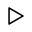
\includegraphics{./img/play.png}

\begin{Shaded}
\begin{Highlighting}[]
\NormalTok{Introdueix el número del DNI: }\DecValTok{12345678}
\NormalTok{Introdueix la lletra del DNI: B}

\NormalTok{El DNI introduit és: }\DecValTok{12345678}\NormalTok{-B}
\end{Highlighting}
\end{Shaded}

En cas de necessitat, amb \texttt{getChar()} es pot guardar el caràcter
del buffer en una variable, per tal de tractar-lo posteriorment:


\includegraphics{./img/c.png}

\begin{Shaded}
\begin{Highlighting}[]
\DataTypeTok{char}\NormalTok{ nomVariable;}
\NormalTok{nomVariable = getChar();}
\end{Highlighting}
\end{Shaded}

\section{Lectura de float en C}\label{lectura-de-float-en-c}

El separador de valors decimals (tipus \texttt{float}) en C \textbf{és
el punt}, no la coma. Per aquest motiu quan s'introdueix un valor
decimal des de teclat, sempre ho farem amb un punt:

Exemple:


\includegraphics{./img/c.png}

\begin{Shaded}
\begin{Highlighting}[]
\PreprocessorTok{#include }\ImportTok{<stdio.h>}

\DataTypeTok{int}\NormalTok{ main(}\DataTypeTok{int}\NormalTok{ argc, }\DataTypeTok{char}\NormalTok{ **argv) \{\}}

    \CommentTok{/* Variable que contindrà el pes d’una persona */}
    \DataTypeTok{float}\NormalTok{ pes;}

    \CommentTok{/* Lectura de la dada per teclat (el separador de decimals és un . ) */}
\NormalTok{    printf(}\StringTok{"Introdueix el pes (kg) d’una persona : "}\NormalTok{);}
\NormalTok{    scanf(}\StringTok{"%f"}\NormalTok{, &pes);}

   \CommentTok{/* Es mostra el valor decimal per pantalla */}
\NormalTok{   printf(}\StringTok{"Has introduit el pes = %.1f kg.}\SpecialCharTok{\textbackslash{}n}\StringTok{"}\NormalTok{, pes);}
   \ControlFlowTok{return} \DecValTok{0}\NormalTok{;}
\NormalTok{\}}
\end{Highlighting}
\end{Shaded}

L'execució serà:

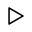
\includegraphics{./img/play.png}

\begin{Shaded}
\begin{Highlighting}[]
\NormalTok{Introdueix el pes (kg) d’una persona : }\FloatTok{79.440}
\NormalTok{Has introduit el pes = }\FloatTok{79.4}\NormalTok{ kg.}
\end{Highlighting}
\end{Shaded}

\chapter{PAC02}\label{pac02}

\section{Booleans en C}\label{booleans}

Alguns punts a considerar amb els booleans en C:

\begin{itemize}
\tightlist
\item
  Quan utilitzem el tipus \texttt{bool} de C ens cal importar la
  llibreria \texttt{\textless{}stdbool.h\textgreater{}}, ja que el tipus
  \texttt{bool} no es va definir a les primeres versions del llenguatge
  C.
\item
  Els valors que pot prendre una variable booleana en C són
  \texttt{false} i \texttt{true}. El llenguatge C tracta internament
  aquests valors com a enters: \texttt{false} correspon a \texttt{0} i
  \texttt{true} a \texttt{1}.
\item
  Quan vulguem introduïr el valor d'un booleà per teclat o bé mostrar-lo
  per pantalla, utilitzarem l'enter \texttt{0} per referir-nos a
  \texttt{false} i \texttt{1} per \texttt{true}.
\item
  L'especificador de tipus dels booleans és \texttt{\%d}.
\item
  Per mostrar el valor d'una variable booleana en C ho podem fer de la
  següent forma:

  
\includegraphics{./img/c.png}

\begin{Shaded}
\begin{Highlighting}[]
\NormalTok{bool isVocal;}
\NormalTok{printf(}\StringTok{"La lletra %c és una vocal (0=false, 1=true) ? %d}\SpecialCharTok{\textbackslash{}n}\StringTok{"}\NormalTok{, lletra, isVocal);}
\end{Highlighting}
\end{Shaded}
\item
  Per llegir un booleà des de teclat, ho faríem de la següent forma:

  
\includegraphics{./img/c.png}

\begin{Shaded}
\begin{Highlighting}[]
\NormalTok{bool variable;}
\NormalTok{scanf(}\StringTok{"%d"}\NormalTok{, &variable);}
\end{Highlighting}
\end{Shaded}
\item
  La lectura per teclat d'un booleà, feta tal i com s'indica al punt
  anterior, generarà un \emph{warning} del següent tipus:
  \texttt{warning:\ format\ \textquotesingle{}\%d\textquotesingle{}\ expects\ argument\ of\ type\ \textquotesingle{}int\ *\textquotesingle{},\ but\ argument\ 2\ has\ type\ \textquotesingle{}\_Bool\ *\textquotesingle{}\ {[}-Wformat={]}}.
  Aquest avís significa que estem utilitzant un especificador de tipus
  (\texttt{\%d}) diferent del que li correspondria al tipus
  \texttt{bool}, el qual treballa únicament amb 1 bit. Com que C no
  disposa de cap especificador de tipus que treballi només amb 1 bit,
  podem fer dues coses:

  \begin{itemize}
  \tightlist
  \item
    Utilitzar una variable auxiliar que ens ajudi a fer una conversió
    intermitja a \texttt{int}, per tal de transformar posteriorment el
    valor a \texttt{bool}:

    
\includegraphics{./img/c.png}

\begin{Shaded}
\begin{Highlighting}[]
\NormalTok{bool variable;}
\DataTypeTok{int}\NormalTok{ aux;}
\NormalTok{scanf(}\StringTok{"%d"}\NormalTok{, &aux);}
\NormalTok{variable = aux;}
\end{Highlighting}
\end{Shaded}
  \item
    Ignorar el warning d'aquesta situació específica: tot i l'avís, el
    programa es pot compilar i executar.
  \end{itemize}
\end{itemize}

\section{Booleans definits com a
enumeratius}\label{booleans-definits-com-a-enumeratius}

En semestres anteriors de l'assignatura de \textbf{Fonaments de
Programació}, s'utilitzava un \textbf{enumeratiu} per definir el tipus
booleà:


\includegraphics{./img/c.png}

\begin{Shaded}
\begin{Highlighting}[]
\KeywordTok{typedef} \KeywordTok{enum}\NormalTok{ \{FALSE, TRUE\} boolean;}
\end{Highlighting}
\end{Shaded}

Aquesta forma de definir el tipus booleà és \textbf{obsoleta} i
\textbf{no s'utilitza} aquest semestre; tal i com s'ha comentat a
l'apartat \ref{booleans}, els booleans els definirem mitjançant la
llibreria \texttt{\textless{}stdbool.h\textgreater{}}. Tingueu-ho
present quan consulteu PAC\footnote{Prova d'Avaluació Continua},
PR\footnote{Pràctica} i PS\footnote{Prova de Síntesi} de semestres
anteriors, en els quals s'utilitzava la nomenclatura ara obsoleta.

\section{Constants: define vs const}\label{constants-define-vs-const}

La definició de constants tant es pot fer amb \texttt{define} com amb
\texttt{const}. Tot i això, la forma de comportar-se d'aquestes dues
opcions és completament diferent, si ve el resultat final és el mateix:

\begin{itemize}
\tightlist
\item
  \texttt{define}: quan utilitzem aquesta opció no es desa en cap
  posició de memòria el valor de la constant. El que es fa realment és
  que en els passos previs a la pròpia compilació del programa, el
  preprocessador substitueix totes les referencies del define pel valor
  indicat.
\end{itemize}

Per exemple, si tenim el següent programa amb una constant creada amb
\texttt{define} :


\includegraphics{./img/c.png}

\begin{Shaded}
\begin{Highlighting}[]
\PreprocessorTok{#include }\ImportTok{<stdio.h>}
\PreprocessorTok{#define MIDA 8}

\DataTypeTok{char}\NormalTok{ lletres[] = \{}\CharTok{'a'}\NormalTok{, }\CharTok{'b'}\NormalTok{, }\CharTok{'c'}\NormalTok{, }\CharTok{'d'}\NormalTok{, }\CharTok{'e'}\NormalTok{, }\CharTok{'f'}\NormalTok{, }\CharTok{'g'}\NormalTok{, }\CharTok{'h'}\NormalTok{\};}
\DataTypeTok{int}\NormalTok{ vertical, horitzontal;}

\DataTypeTok{int}\NormalTok{ main(}\DataTypeTok{int}\NormalTok{ argc, }\DataTypeTok{char}\NormalTok{ **argv) \{}
    \CommentTok{/* font: https://en.wikipedia.org/wiki/Chess */}

    \ControlFlowTok{for}\NormalTok{ (vertical=MIDA; vertical>=}\DecValTok{1}\NormalTok{; vertical--) \{}
        \ControlFlowTok{for}\NormalTok{ (horitzontal=}\DecValTok{0}\NormalTok{; horitzontal<=MIDA-}\DecValTok{1}\NormalTok{; horitzontal++) \{}
\NormalTok{            printf(}\StringTok{"%c%d "}\NormalTok{, lletres[horitzontal], vertical);}
\NormalTok{        \}}
\NormalTok{        printf(}\StringTok{"}\SpecialCharTok{\textbackslash{}n}\StringTok{"}\NormalTok{);}
\NormalTok{    \}}
\NormalTok{\}}
\end{Highlighting}
\end{Shaded}

Abans de la compilació, el preprocessador entre altres accions elimina
comentaris i substitueix totes les referències \texttt{MIDA} per
\texttt{8}:


\includegraphics{./img/c.png}

\begin{Shaded}
\begin{Highlighting}[]
\PreprocessorTok{#include }\ImportTok{<stdio.h>}

\DataTypeTok{char}\NormalTok{ lletres[] = \{}\CharTok{'a'}\NormalTok{, }\CharTok{'b'}\NormalTok{, }\CharTok{'c'}\NormalTok{, }\CharTok{'d'}\NormalTok{, }\CharTok{'e'}\NormalTok{, }\CharTok{'f'}\NormalTok{, }\CharTok{'g'}\NormalTok{, }\CharTok{'h'}\NormalTok{\};}
\DataTypeTok{int}\NormalTok{ vertical, horitzontal;}

\DataTypeTok{int}\NormalTok{ main(}\DataTypeTok{int}\NormalTok{ argc, }\DataTypeTok{char}\NormalTok{ **argv) \{}

    \ControlFlowTok{for}\NormalTok{ (vertical=}\DecValTok{8}\NormalTok{; vertical>=}\DecValTok{1}\NormalTok{; vertical--) \{}
        \ControlFlowTok{for}\NormalTok{ (horitzontal=}\DecValTok{0}\NormalTok{; horitzontal<=}\DecValTok{8}\NormalTok{-}\DecValTok{1}\NormalTok{; horitzontal++) \{}
\NormalTok{            printf(}\StringTok{"%c%d "}\NormalTok{, lletres[horitzontal], vertical);}
\NormalTok{        \}}
\NormalTok{        printf(}\StringTok{"}\SpecialCharTok{\textbackslash{}n}\StringTok{"}\NormalTok{);}
\NormalTok{    \}}
\NormalTok{\}}
\end{Highlighting}
\end{Shaded}

Per tant la definició de constants amb \texttt{define} es comporta com
si d'un ``cercar-reemplaçar'' d'un processador de textos es tractés. No
es desa cap constant en memòria, però per contra, el programa ocuparà
una mica més per la substitució directa de referències que fa; la
substitució la fa en tot el programa, no es pot limitar a un àmbit
concret (per exemple només dins d'una funció).

\begin{itemize}
\tightlist
\item
  \texttt{const}: en aquest cas sí que es reserva una posició de
  memòria. En C es comporta igual com si fos una variable, però la qual
  únicament funciona en mode lectura: no li podem modificar el valor.
\end{itemize}

A més, \texttt{const} ens permet també dir quin tipus de valor tindrà la
constant: si és de tipus \texttt{float}, \texttt{int},
\texttt{char}\ldots{} amb el que aquest fet ens dóna un punt addicional
de control, ja que ens assegurem que el tipus de valor assignat serà el
correcte pel programa.

Amb aquest tipus de definició de constant, l'exemple anterior quedaria
de la següent forma:


\includegraphics{./img/c.png}

\begin{Shaded}
\begin{Highlighting}[]
\PreprocessorTok{#include }\ImportTok{<stdio.h>}
\DataTypeTok{const} \DataTypeTok{int}\NormalTok{ MIDA }\DecValTok{8}

\DataTypeTok{char}\NormalTok{ lletres[] = \{}\CharTok{'a'}\NormalTok{, }\CharTok{'b'}\NormalTok{, }\CharTok{'c'}\NormalTok{, }\CharTok{'d'}\NormalTok{, }\CharTok{'e'}\NormalTok{, }\CharTok{'f'}\NormalTok{, }\CharTok{'g'}\NormalTok{, }\CharTok{'h'}\NormalTok{\};}
\DataTypeTok{int}\NormalTok{ vertical, horitzontal;}

\DataTypeTok{int}\NormalTok{ main(}\DataTypeTok{int}\NormalTok{ argc, }\DataTypeTok{char}\NormalTok{ **argv) \{}

    \CommentTok{/* La constant MIDA està desada en memòria */}
\NormalTok{    printf(}\StringTok{"posició en memòria de la constant MIDA : %p }\SpecialCharTok{\textbackslash{}n}\StringTok{"}\NormalTok{, &MIDA);}

    \ControlFlowTok{for}\NormalTok{ (vertical=MIDA; vertical>=}\DecValTok{1}\NormalTok{; vertical--) \{}
        \ControlFlowTok{for}\NormalTok{ (horitzontal=}\DecValTok{0}\NormalTok{; horitzontal<=MIDA-}\DecValTok{1}\NormalTok{; horitzontal++) \{}
\NormalTok{            printf(}\StringTok{"%c%d "}\NormalTok{, lletres[horitzontal], vertical);}
\NormalTok{        \}}
\NormalTok{        printf(}\StringTok{"}\SpecialCharTok{\textbackslash{}n}\StringTok{"}\NormalTok{);}
\NormalTok{    \}}
\NormalTok{\}}
\end{Highlighting}
\end{Shaded}

Com es pot veure, és possible obtinir l'adreça en memòria on es desa la
constant \texttt{MIDA}. En aquest cas, sí que pots definir una constant
amb \texttt{const} i fer que només afecti un àmbit determinat (per
exemple, que la constant estigui definida únicament dins d'una funció).

Aquestes són les principals diferències entre \texttt{define} i
\texttt{const} a l'hora de definir una constant; \texttt{define} es va
crear molt abans que no la sentència \texttt{const}, amb el que és un
habit força habitual decantar-se per aquesta opció per temes més
històrics.

\section{Com mostrar el valor d'una
constant}\label{com-mostrar-el-valor-duna-constant}

En C podem mostrar per pantalla el valor d'una constant definida amb
\texttt{\#define} mitjançant \texttt{printf()}. Exemple:


\includegraphics{./img/c.png}

\begin{Shaded}
\begin{Highlighting}[]
\PreprocessorTok{#include }\ImportTok{<stdio.h>}

\PreprocessorTok{#define PARAULA "world"}
\PreprocessorTok{#define ANY 2019}
\PreprocessorTok{#define EXCLAMACIO '!'}

\DataTypeTok{int}\NormalTok{ main(}\DataTypeTok{int}\NormalTok{ argc, }\DataTypeTok{char}\NormalTok{ **argv) \{}
\NormalTok{    printf(}\StringTok{"hello %s and happy %d %c}\SpecialCharTok{\textbackslash{}n}\StringTok{"}\NormalTok{, PARAULA, ANY, EXCLAMACIO);}
    \ControlFlowTok{return} \DecValTok{0}\NormalTok{;}
\NormalTok{\}}
\end{Highlighting}
\end{Shaded}

El resultat que es mostrarà per pantalla serà:

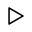
\includegraphics{./img/play.png}

\begin{Shaded}
\begin{Highlighting}[]
\NormalTok{hello world and happy }\DecValTok{2019}\NormalTok{ !}
\end{Highlighting}
\end{Shaded}

\section{Precisió en variables float}\label{precisio-en-variables-float}

Hi ha alguns valors decimals determinats que no es poden representar de
forma precisa en una variable de tipus \texttt{float}. La millor solució
pels casos que tractem és arrodonir al número de decimals que realment
necessitem.

Si en canvi volem sí o sí treballar amb tots els decimals, podem optar
per utilitzar un tipus de dada que tingui major precisió que
\texttt{float}: \texttt{double}.

Per exemple, el següent programa retorna el resultat esperat si es desa
en un \texttt{double}, i no així si es fa en un \texttt{float}:


\includegraphics{./img/c.png}

\begin{Shaded}
\begin{Highlighting}[]
\PreprocessorTok{#include }\ImportTok{<stdio.h>}

\DataTypeTok{int}\NormalTok{ main(}\DataTypeTok{int}\NormalTok{ argc, }\DataTypeTok{char}\NormalTok{ **argv) \{ }

    \DataTypeTok{float}\NormalTok{ num1; }
    \DataTypeTok{float}\NormalTok{ num2;}
    \DataTypeTok{float}\NormalTok{ resultat1; }
    \DataTypeTok{double}\NormalTok{ resultat2; }
    
\NormalTok{    num1 = }\FloatTok{1.3}\NormalTok{; }
\NormalTok{    num2 = }\DecValTok{17}\NormalTok{;}
\NormalTok{    resultat1 = num1 + num2; }
\NormalTok{    printf(}\StringTok{"resultat amb float: %f}\SpecialCharTok{\textbackslash{}n}\StringTok{"}\NormalTok{, resultat1); }
\NormalTok{    resultat2 = num1 + num2; }
\NormalTok{    printf(}\StringTok{"resultat amb double: %f}\SpecialCharTok{\textbackslash{}n}\StringTok{"}\NormalTok{, resultat2); }
    \ControlFlowTok{return} \DecValTok{0}\NormalTok{; }
\NormalTok{\}}
\end{Highlighting}
\end{Shaded}

La sortida que genera és:

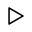
\includegraphics{./img/play.png}

\begin{Shaded}
\begin{Highlighting}[]
\NormalTok{resultat amb  }\DataTypeTok{float}\NormalTok{: }\FloatTok{18.299999}
\NormalTok{resultat amb }\DataTypeTok{double}\NormalTok{: }\FloatTok{18.300000}
\end{Highlighting}
\end{Shaded}

\section{Semàntica d'una expressió}\label{semantica-duna-expressio}

Si recordem el que es comenta al punt \textbf{3.2. Semàntica d'una
expressió} del mòdul de la xWiki \textbf{Tipus bàsics de dades}, hem
d'aconseguir queles expressions i comparacions realitzades als
algorismes siguin \textbf{semànticament correctes}.

Amb un exemple es veurà més clar: tenim el següent algorisme que indica
si una persona és major d'edat. Fixeu-vos que l'expressió realitza una
comparació entre dos enters: la variable \texttt{edat} i el número
\texttt{17}.

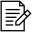
\includegraphics{./img/alg.png}

\begin{verbatim}
var
    edat: int;
    majorEdat: boolean;
end var

algorithm serMajorEdat

    writeString("Introdueix edat del conductor :");
    edat := readInteger();

    majorEdat := (edat > 17);

    writeString("El conductor és major d'edat? :");
    writeBoolean(majorEdat);

end algorithm
\end{verbatim}

Aquesta expressió \textbf{és semànticament correcta}.

En canvi, imaginem ara que el nostre algorisme accepta decimals per
l'\texttt{edat}; per exemple, \texttt{19.5} indicaria que l'edat és de
19 anys i 6 mesos. Així tenim el següent plantejament, on ara la
variable \texttt{edat} és de tipus \texttt{real}:

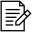
\includegraphics{./img/alg.png}

\begin{verbatim}
var
    edat: real;
    majorEdat: boolean;
end var

algorithm serMajorEdat

    writeString("Introdueix edat del conductor :");
    edat := readReal();

    majorEdat := (edat > 17);

    writeString("El conductor és major d'edat? :");
    writeBoolean(majorEdat);

end algorithm
\end{verbatim}

L'algorisme ara \textbf{no és correcte} ja que conté una expressió
\textbf{semànticament incorrecta}, en la qual es compara \texttt{edat}
(real) amb \texttt{17} (enter). Per solucionar-ho, podem utilitzar
alguna de les funcions de conversió comentades a l'apartat \textbf{4.
Funcions de conversió de tipus del mateix mòdul}:

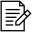
\includegraphics{./img/alg.png}

\begin{verbatim}
{opció 1: fem que els dos valors siguin de tipus enter}
majorEdat := (realToInteger(edat) > 17);    

{opció 2: fem que els dos valors siguin de tipus real}
majorEdat := (edat > integerToReal(17));
\end{verbatim}

\section{Exemples d'expressions}\label{exemples-dexpressions}

\subsection{Exemple 1: esParell}\label{exemple-1-esparell}

Imaginem que ens demanen un algorisme que indiqui si un número és
parell.

Una possible solució seria:

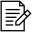
\includegraphics{./img/alg.png}

\begin{verbatim}
algorithm esParell
    var
        numero: integer;
        isParell: boolean;
    end var

    writeString("Introdueix un número : ");
    numero:= readInteger();
    isParell:= (numero mod 2 = 0);
    
    writeString("El numero ");
    writeInteger(numero);
    writeString(" és parell? ");
    writeBoolean(isParell);

end algorithm
\end{verbatim}

La variable \texttt{isParell} prendrà el valor \texttt{TRUE} si el
número es parell i \texttt{FALSE} en cas contrari. No ha calgut
utilitzar cap estructura \texttt{if-else} per resoldre l'algorisme.

Una possible forma de codificar-ho en llenguatge C és:


\includegraphics{./img/c.png}

\begin{Shaded}
\begin{Highlighting}[]
\PreprocessorTok{#include }\ImportTok{<stdio.h>}
\PreprocessorTok{#include }\ImportTok{<stdbool.h>}

\DataTypeTok{int}\NormalTok{ main(}\DataTypeTok{int}\NormalTok{ argc, }\DataTypeTok{char}\NormalTok{ **argv) \{}

    \DataTypeTok{int}\NormalTok{ numero;}
\NormalTok{    bool isParell;}

\NormalTok{    printf(}\StringTok{"Introdueix un número : "}\NormalTok{);}
\NormalTok{    scanf(}\StringTok{"%d"}\NormalTok{, &numero);}
\NormalTok{    isParell = (numero % }\DecValTok{2}\NormalTok{ == }\DecValTok{0}\NormalTok{);}
    
\NormalTok{    printf(}\StringTok{"El número %d és parell? (0=FALSE, 1=TRUE) : %d }\SpecialCharTok{\textbackslash{}n}\StringTok{"}\NormalTok{, numero, isParell);}

    \ControlFlowTok{return} \DecValTok{0}\NormalTok{;}
\NormalTok{\}}
\end{Highlighting}
\end{Shaded}

\subsection{Exemple 2: capDeSetmana}\label{exemple-2-capdesetmana}

Imaginem que volem fer un programa molt senzill que ens digui si avui és
cap de setmana o no. El seu algorisme seria el següent:

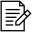
\includegraphics{./img/alg.png}

\begin{verbatim}
type
    dies = {DILLUNS, DIMARTS, DIMECRES, DIJOUS, DIVENDRES, DISSABTE, DIUMENGE};
end type

algorithm capDeSetmana

    var
        esCapDeSetmana: boolean;
        diaSetmana: dies;
    end var

    writeString("Quin dia de la setmana és avui ?\n");
    writeString("Per DILLUNS tecleja 0\n");
    writeString("Per DIMARTS tecleja 1\n");
    writeString("Per DIMECRES tecleja 2\n");
    writeString("Per DIJOUS tecleja 3\n");
    writeString("Per DIVENDRES tecleja 4\n");
    writeString("Per DISSABTE tecleja 5\n");
    writeString("Per DIUMENGE tecleja 6\n");
 
    diaSetmana:= readInteger();
    esCapDeSetmana:= (diaSetmana = DISSABTE or diaSetmana = DIUMENGE);

    writeString("Avui és cap de setmana?");
    writeBool(esCapDeSetmana);

end algorithm
\end{verbatim}

La variable \texttt{boolean} \texttt{esCapDeSetmana} prendrà el valor de
\texttt{true} o \texttt{false} en funció del resultat d'avaluar
l'expressió. No és necessari la utilització d'estructures condicionals
\texttt{if-else} que veurem més endavant en el curs.

Una possible forma de codificar-ho en llenguatge C és:


\includegraphics{./img/c.png}

\begin{Shaded}
\begin{Highlighting}[]
\PreprocessorTok{#include }\ImportTok{<stdio.h>}
\PreprocessorTok{#include }\ImportTok{<stdbool.h>}

\KeywordTok{typedef} \KeywordTok{enum}\NormalTok{ \{DILLUNS, DIMARTS, DIMECRES, DIJOUS, DIVENDRES, DISSABTE, DIUMENGE\} dies;}

\DataTypeTok{int}\NormalTok{ main(}\DataTypeTok{int}\NormalTok{ argc, }\DataTypeTok{char}\NormalTok{ **argv) \{}

\NormalTok{    bool esCapDeSetmana;}
\NormalTok{    dies diaSetmana;}

\NormalTok{    printf(}\StringTok{"}\SpecialCharTok{\textbackslash{}n}\StringTok{Quin dia de la setmana és avui ?}\SpecialCharTok{\textbackslash{}n}\StringTok{"}\NormalTok{);}
\NormalTok{    printf(}\StringTok{"Per DILLUNS tecleja 0}\SpecialCharTok{\textbackslash{}n}\StringTok{"}\NormalTok{);}
\NormalTok{    printf(}\StringTok{"Per DIMARTS tecleja 1}\SpecialCharTok{\textbackslash{}n}\StringTok{"}\NormalTok{);}
\NormalTok{    printf(}\StringTok{"Per DIMECRES tecleja 2}\SpecialCharTok{\textbackslash{}n}\StringTok{"}\NormalTok{);}
\NormalTok{    printf(}\StringTok{"Per DIJOUS tecleja 3}\SpecialCharTok{\textbackslash{}n}\StringTok{"}\NormalTok{);}
\NormalTok{    printf(}\StringTok{"Per DIVENDRES tecleja 4}\SpecialCharTok{\textbackslash{}n}\StringTok{"}\NormalTok{);}
\NormalTok{    printf(}\StringTok{"Per DISSABTE tecleja 5}\SpecialCharTok{\textbackslash{}n}\StringTok{"}\NormalTok{);}
\NormalTok{    printf(}\StringTok{"Per DIUMENGE tecleja 6}\SpecialCharTok{\textbackslash{}n}\StringTok{"}\NormalTok{);}

\NormalTok{    scanf(}\StringTok{"%u"}\NormalTok{, &diaSetmana);}
\NormalTok{    esCapDeSetmana = (diaSetmana == DISSABTE || diaSetmana == DIUMENGE);}

\NormalTok{    printf(}\StringTok{"Avui és cap de setmana (0 == false, 1 == true) ? %d}\SpecialCharTok{\textbackslash{}n}\StringTok{"}\NormalTok{, esCapDeSetmana);}

    \ControlFlowTok{return} \DecValTok{0}\NormalTok{;}
\NormalTok{\}}
\end{Highlighting}
\end{Shaded}

Varis punts a considerar:

\begin{itemize}
\tightlist
\item
  Recordem que inicialment en C no existia el tipus booleà. Per poder
  utilitzar \texttt{bool}, i els valors \texttt{true} i \texttt{false}
  ens cal importar prèviament la llibreria
  \texttt{\textless{}stdbool.h\textgreater{}}.
\item
  L'especificador de tipus d'un \texttt{bool} és \texttt{\%d}.
\item
  Quan definim una variable de tipus \texttt{enum}, utilitzem
  l'especificador de tipus \texttt{\%u}. Ho podríem fer com a
  \texttt{\%d}, però us retornarà un warning tot i que el resultat sigui
  correcte. El tipus \texttt{\%u} és igual que un enter \texttt{\%d}
  però sense signe: això significa que amb \texttt{\%d} podem tractar
  valors negatius com -12 i amb \texttt{\%u} això no és possible, però
  com que sabem que els valors que pot prendre un \texttt{enum} sempre
  seran \textgreater{}= 0, ens convé utilitzar \texttt{\%u}.
\item
  Per les particularitats dels \texttt{bool} en el llenguatge de
  programació C que ja hem comentat anteriorment, l'entrada i sortida de
  valors d'un \texttt{boolean} serà numèrica. Per facilitar la
  comprensió podem mostrar per pantalla un literal que ens indiqui que
  \texttt{0} equival a \texttt{false} i \texttt{1} a \texttt{true}.
\end{itemize}

\subsection{Exemple 3: esVocal}\label{exemple-3-esvocal}

Exemple: volem fer un programa que, entrat un caràcter pel canal
d'entrada, ens indiqui si es tracta o no d'una vocal.

Una possible solució per l'algorisme és la següent:

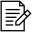
\includegraphics{./img/alg.png}

\begin{verbatim}
var
    lletra: char;
    isVocal: boolean;
end var

algorithm trobaVocal

    writeString("Tecleja una lletra :");
    lletra := readChar();

    { en aquest exemple només tractem les vocals minúscules }
    isVocal := lletra = 'a' or lletra = 'e' or lletra = 'i' or lletra = 'o' or lletra = 'u';

    writeString("La lletra ");
    writeChar(lletra);
    writeString(" és una vocal? ");
    writeBoolean(isVocal);

end algorithm
\end{verbatim}

Com es pot veure el plantejament de l'algorisme és:

\begin{itemize}
\tightlist
\item
  Llegim un caràcter des del canal d'entrada.
\item
  Comparem el caràcter amb a, e, i, o, u.

  \begin{itemize}
  \tightlist
  \item
    Si coincideix amb alguna d'aquestes vocals, la variable isVocal :=
    true.
  \item
    Si no coincideix amb cap de les vocals, la variable isVocal :=
    false.
  \end{itemize}
\item
  Es mostra el resultat per pantalla.
\end{itemize}

Com ho podem traduir a llenguatge C? Una possible opció és:


\includegraphics{./img/c.png}

\begin{Shaded}
\begin{Highlighting}[]
\PreprocessorTok{#include }\ImportTok{<stdio.h>}
\PreprocessorTok{#include }\ImportTok{<stdbool.h>}

\DataTypeTok{int}\NormalTok{ main(}\DataTypeTok{int}\NormalTok{ argc, }\DataTypeTok{char}\NormalTok{ **argv) \{}

    \DataTypeTok{char}\NormalTok{ lletra;}
\NormalTok{    bool isVocal;}

\NormalTok{    printf(}\StringTok{"Introdueix una lletra : "}\NormalTok{);}
\NormalTok{    scanf(}\StringTok{"%c"}\NormalTok{, &lletra);}

    \CommentTok{/* en aquest exemple només tractem les vocals minúscules */}
\NormalTok{    isVocal = lletra == }\CharTok{'a'}\NormalTok{ || lletra == }\CharTok{'e'}\NormalTok{ || lletra == }\CharTok{'i'}\NormalTok{ || lletra == }\CharTok{'o'}\NormalTok{ || lletra == }\CharTok{'u'}\NormalTok{;}

\NormalTok{    printf(}\StringTok{"La lletra %c és una vocal (0=FALSE, 1=TRUE) ? %d}\SpecialCharTok{\textbackslash{}n}\StringTok{"}\NormalTok{, lletra, isVocal);}

    \ControlFlowTok{return} \DecValTok{0}\NormalTok{;}
\NormalTok{\}}
\end{Highlighting}
\end{Shaded}

\subsection{Exemple 4: votacions}\label{exemple-4-votacions}

Imaginem que hem de fer un programa que validi si una persona pot anar a
votar o no; la condició que ens diuen que cal complir és que la persona
sigui major d'edat i a més estigui al cens electoral de la localitat on
està votant.

L'algorisme podria ser el següent:

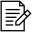
\includegraphics{./img/alg.png}

\begin{verbatim}
algorithm votacions
    var
        isMajorEdat: boolean;
        isCensat: boolean;
        isVotar: boolean;
    end var
    
    writeString("Ets major d'edat (0=FALSE, 1=TRUE) ? : ");
    isMajorEdat := readBoolean();
    writeString("Estàs al cens electoral (0=FALSE, 1=TRUE) ? : ");
    isCensat := readBoolean();
    
    { expressió }
    isVotar := isMajorEdat and isCensat;

    writeString("Pots anar a votar (0=FALSE, 1=TRUE) :");
    writeBoolean(isVotar);

end algorithm
\end{verbatim}

Una possible implementació en C seria:


\includegraphics{./img/c.png}

\begin{Shaded}
\begin{Highlighting}[]
\PreprocessorTok{#include }\ImportTok{<stdio.h>}
\PreprocessorTok{#include }\ImportTok{<stdbool.h>}

\DataTypeTok{int}\NormalTok{ main(}\DataTypeTok{int}\NormalTok{ argc, }\DataTypeTok{char}\NormalTok{ **argv) \{}

\NormalTok{    bool isMajorEdat;}
\NormalTok{    bool isCensat;}
\NormalTok{    bool isVotar;}

\NormalTok{    printf(}\StringTok{"Ets major d'edat (0=FALSE, 1=TRUE) ? : "}\NormalTok{);}
\NormalTok{    scanf(}\StringTok{"%d"}\NormalTok{, &isMajorEdat);}

\NormalTok{    printf(}\StringTok{"Estàs al cens electoral (0=FALSE, 1=TRUE) ? : "}\NormalTok{);}
\NormalTok{    scanf(}\StringTok{"%d"}\NormalTok{, &isCensat);}

\NormalTok{    \{ expressió \}}
\NormalTok{    isVotar = isMajorEdat && isCensat;}

\NormalTok{    printf(}\StringTok{"Pots anar a votar (0=FALSE, 1=TRUE) : %d}\SpecialCharTok{\textbackslash{}n}\StringTok{"}\NormalTok{, isVotar);}

    \ControlFlowTok{return} \DecValTok{0}\NormalTok{;}
\NormalTok{\}}
\end{Highlighting}
\end{Shaded}

Un possible execució d'aquest exemple seria:

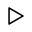
\includegraphics{./img/play.png}

\begin{Shaded}
\begin{Highlighting}[]
\NormalTok{Ets major d'edat (}\DecValTok{0}\NormalTok{=FALSE, }\DecValTok{1}\NormalTok{=TRUE) ? : }\DecValTok{1}
\NormalTok{Estàs al cens electoral (}\DecValTok{0}\NormalTok{=FALSE, }\DecValTok{1}\NormalTok{=TRUE) ? : }\DecValTok{0}
\NormalTok{Pots anar a votar (}\DecValTok{0}\NormalTok{=FALSE, }\DecValTok{1}\NormalTok{=TRUE) : }\DecValTok{0}
\end{Highlighting}
\end{Shaded}

\subsection{Exemple 5:
ginTonicPreparation}\label{exemple-5-gintonicpreparation}

Imaginem que volem preparar un gintònic. Sabem el volum de ginebra i de
tònica que utilitzarem, i quina és la capacitat de la copa de baló que
el contindrà.

Hem vist una oferta per internet i hem comprat glaçons metàl·lics d'acer
inoxidable\ldots{} però se'ns ha anat una mica el cap i n'hem comprat un
total de 20 unitats.

Volem fer un programa que, utilitzant únicament expressions, ens digui
si podem preparar o no el gintònic en funció del número de glaçons que
li volem posar:

\begin{itemize}
\tightlist
\item
  si el nombre de glaçons caben dins de la copa, retornarà
  \texttt{true}.
\item
  en cas contrari, retornarà \texttt{false}.
\end{itemize}

Per tant el que ha de fer el nostre programa bàsicament és validar si el
volum de ginebra + tònica + (glaço) * número de glaçons supera o no el
volum de la copa.

L'algorisme podria ser el següent:

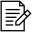
\includegraphics{./img/alg.png}

\begin{verbatim}
const
    GIN: real = 50.0;              { in ml }
    TONIC: real = 200.0;           { in ml }
    GLASS: real = 620.0;           { in ml }
    METAL_ICE_CUBE: real = 42.875; { in ml }
end const

algorithm ginTonicPreparation

    var
        numMetalIceCubes: integer;
        isPossible: boolean;
    end var

    writeString("Number of metal ice cubes ? (integer) : ");
    numMetalIceCubes:= readInteger();

    isPossible:= (GLASS ≥ (GIN + TONIC + METAL_ICE_CUBE * numMetalIceCubes));

    writeString("Can you make a gin & tonic? : ");
    writeBoolean(isPossible);

end algorithm
\end{verbatim}

L'expressió que dóna valor a \texttt{isPossible} s'ocupa d'avaluar el
volum de la copa respecte el resultant de ginebra, tònica i glaçons.

La seva traducció a C podria ser:


\includegraphics{./img/c.png}

\begin{Shaded}
\begin{Highlighting}[]
\PreprocessorTok{#include }\ImportTok{<stdio.h>}
\PreprocessorTok{#include }\ImportTok{<stdbool.h>}

\PreprocessorTok{#define GIN 50.0              }\CommentTok{/* in ml */}
\PreprocessorTok{#define TONIC 200.0           }\CommentTok{/* in ml */}
\PreprocessorTok{#define GLASS 620.0           }\CommentTok{/* in ml */}
\PreprocessorTok{#define METAL_ICE_CUBE 42.875 }\CommentTok{/* in ml */}\PreprocessorTok{ }

\DataTypeTok{int}\NormalTok{ main(}\DataTypeTok{int}\NormalTok{ argc, }\DataTypeTok{char}\NormalTok{ **argv) \{}

    \DataTypeTok{int}\NormalTok{ numMetalIceCubes;}
\NormalTok{    bool isPossible;}

\NormalTok{    printf(}\StringTok{"Number of metal ice cubes ? (integer) : "}\NormalTok{);}
\NormalTok{    scanf(}\StringTok{"%d"}\NormalTok{, &numMetalIceCubes);}

\NormalTok{    isPossible = GLASS >= (GIN + TONIC + METAL_ICE_CUBE * numMetalIceCubes);}

\NormalTok{    printf(}\StringTok{"Can you make a gin & tonic? (0=FALSE, 1=TRUE) : %d}\SpecialCharTok{\textbackslash{}n}\StringTok{"}\NormalTok{, isPossible);}
    
    \ControlFlowTok{return} \DecValTok{0}\NormalTok{;}
\NormalTok{\}}
\end{Highlighting}
\end{Shaded}

Per realitzar el càlcul en C també s'ha utilitzat una expressió.

\subsection{Exemple 6: ginTonicFreeMl}\label{exemple-6-gintonicfreeml}

Anem a evolucionar l'exemple anterior del gintònic: imaginem ara que
volem que el nostre programa ens digui el volum (en mililitres) que
queda lliure a la copa una vegada posat un determinat nombre de glaçons.

L'algorisme quedaria de la següent forma:

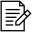
\includegraphics{./img/alg.png}

\begin{verbatim}
const
    GIN: real = 50.0;              { in ml }
    TONIC: real = 200.0;           { in ml }
    GLASS: real = 620.0;           { in ml }
    METAL_ICE_CUBE: real = 42.875; { in ml }
end const

algorithm ginTonicFreeMl

    var
        numMetalIceCubes: integer;
        volumeFree: real;
    end var

    writeString("Number of metal ice cubes ? (integer) : ");
    numMetalIceCubes:= readInteger();

    volumeFree:= GLASS - (GIN + TONIC + METAL_ICE_CUBE * numMetalIceCubes);

    writeString("How many free ml in the glass? : ");
    writeReal(volumeFree);

end algorithm
\end{verbatim}

I la codificació en C :

\includegraphics{./img/c.png}

\begin{Shaded}
\begin{Highlighting}[]
\PreprocessorTok{#include }\ImportTok{<stdio.h>}

\PreprocessorTok{#define GIN 50.0              }\CommentTok{/* in ml */}
\PreprocessorTok{#define TONIC 200.0           }\CommentTok{/* in ml */}
\PreprocessorTok{#define GLASS 620.0           }\CommentTok{/* in ml */}
\PreprocessorTok{#define METAL_ICE_CUBE 42.875 }\CommentTok{/* in ml */}

\DataTypeTok{int}\NormalTok{ main(}\DataTypeTok{int}\NormalTok{ argc, }\DataTypeTok{char}\NormalTok{ **argv) \{}

    \DataTypeTok{int}\NormalTok{ numMetalIceCubes;}
    \DataTypeTok{float}\NormalTok{ volumeFree;}

\NormalTok{    printf(}\StringTok{"Number of metal ice cubes ? (integer) : "}\NormalTok{);}
\NormalTok{    scanf(}\StringTok{"%d"}\NormalTok{, &numMetalIceCubes);}

\NormalTok{    volumeFree = GLASS - (GIN + TONIC + METAL_ICE_CUBE * numMetalIceCubes);}

\NormalTok{    printf(}\StringTok{"How many free ml in the glass ? : %.3f ml }\SpecialCharTok{\textbackslash{}n}\StringTok{"}\NormalTok{, volumeFree);}
    
    \ControlFlowTok{return} \DecValTok{0}\NormalTok{;}
\NormalTok{\}}
\end{Highlighting}
\end{Shaded}

\subsection{Exemple 7: scoutingBasquet}\label{exemple-7-scoutingbasquet}

Imaginem que fem tasques d'scouting per les seccions de bàsquet femení i
masculí del nostre club, i ens han encarregat cobrir alguna de les tres
places següents:

\begin{itemize}
\tightlist
\item
  Per l'equip femení: una pivot que com a mínim faci 195cm d'alçada.
\item
  Per l'equip femení: una base, l'alçada de la qual sigui inferior a
  170cm.
\item
  Per l'equip masculí: un base que sigui més alt de 175cm però a la
  vegada que no superi els 190cm.
\end{itemize}

El nostre programa demanarà per teclat si es tracta d'una jugadora o un
jugador, i quina és la seva alçada. A continuació amb expressions
avaluarà les condicions introduides i si les compleix per alguna de les
tres places disponibles, l'escollirà (\texttt{isDrafted}).

Una possible forma de codificar en C aquest programa seria:

\includegraphics{./img/c.png}

\begin{Shaded}
\begin{Highlighting}[]
\PreprocessorTok{#include }\ImportTok{<stdio.h>}
\PreprocessorTok{#include }\ImportTok{<stdbool.h>}

\KeywordTok{typedef} \KeywordTok{enum}\NormalTok{ \{MALE, FEMALE\} tGender;}

\DataTypeTok{int}\NormalTok{ main(}\DataTypeTok{int}\NormalTok{ argc, }\DataTypeTok{char}\NormalTok{ **argv) \{}

\NormalTok{    bool isPointGuard; }\CommentTok{/* Point Guard = base */}
\NormalTok{    bool isCenter;     }\CommentTok{/* Center = pivot */}
\NormalTok{    bool isDrafted;}
    \DataTypeTok{int}\NormalTok{ height;}
\NormalTok{    tGender gender;}

\NormalTok{    printf(}\StringTok{"Gender (0=MALE, 1=FEMALE) : "}\NormalTok{);}
\NormalTok{    scanf(}\StringTok{"%u"}\NormalTok{, &gender);}
\NormalTok{    printf(}\StringTok{"Heigth (integer value) : "}\NormalTok{);}
\NormalTok{    scanf(}\StringTok{"%d"}\NormalTok{, &height);}

    \CommentTok{/* Primer mirem si la posició de base femení o masculí la podem cobrir o no */}
\NormalTok{    isPointGuard = }
\NormalTok{        (height < }\DecValTok{170}\NormalTok{ && (gender == FEMALE)) ||}
\NormalTok{        (height < }\DecValTok{190}\NormalTok{ && height > }\DecValTok{175}\NormalTok{ && (gender == MALE));}

    \CommentTok{/* A continuació comprovem si es tracta de la pívot femenina que busquem */}
\NormalTok{    isCenter = (height >= }\DecValTok{195}\NormalTok{ && (gender == FEMALE));}

    \CommentTok{/* Només que es compleixi alguna de les dues expressions anteriors }
\CommentTok{       (que isPointGuard sigui TRUE o que isCenter sigui TRUE), el jugador/a }
\CommentTok{       serà escollit per formar part de les nostres seccions de bàsquet */}
\NormalTok{    isDrafted = isPointGuard || isCenter;}

\NormalTok{    printf(}\StringTok{"}\SpecialCharTok{\textbackslash{}n}\StringTok{Is drafted (0=FALSE, 1=TRUE) ? : "}\NormalTok{);}
\NormalTok{    printf(}\StringTok{"%d}\SpecialCharTok{\textbackslash{}n}\StringTok{"}\NormalTok{, isDrafted);}
\NormalTok{\}}
\end{Highlighting}
\end{Shaded}

Fixeu-vos que \texttt{isPointGuard} i \texttt{isCenter} són variables de
tipus \texttt{bool}, ja que l'avaluació de les expressions també serà de
tipus \texttt{bool}.

Hi poden haver altres codificacions igual de vàlides, aquesta no és la
única solució possible.

\chapter{PAC03}\label{pac03}

\section{Com declarar un vector en llenguatge
algorísmic}\label{com-declarar-un-vector-en-llenguatge-algorismic}

Quan es declara un vector en llenguatge algorísmic no cal declarar una
variable per cadascuna de les posicions d'aquest vector.

Per exemple, si volem un algorisme que sumi tres enters continguts dins
d'un vector podem fer el següent:

\includegraphics{./img/alg.png}

\begin{verbatim}
const
    NUM_ENTERS: integer = 3;
end const

algorithm sumaEnters

    var
        vectorEnters: vector[NUM_ENTERS] of integer;
        sumaEnters: integer;
    end var

    vectorEnters[1] := 13;
    vectorEnters[2] := 24;
    vectorEnters[3] := 2;

    { Com es pot veure, accedim directament a les posicions del vector }
    { en comptes de definir una variable per cada posició. }

    sumaEnters := vectorEnters[1] + vectorEnters[2] + vectorEnters[3];

    { Cal recordar també que en llenguatge algorísmic, en un vector de mida n }
    { la primera posició del vector és la 1 i la darrera la n; en canvi en llenguatge C }
    { la primera sempre és la 0 i l'última la n-1. }

    writeString("La suma dels 3 enters del vector és : ");
    writeInteger(sumaEnters);

end algorithm
\end{verbatim}

\section{Significat dels arguments del
main}\label{significat-dels-arguments-del-main}

La principal diferència entre la definició
\texttt{main(int\ argc,\ char\ **argv)} i \texttt{main()} és que la
primera opció està preparada per rebre arguments quan s'executa el
programa i no així la segona.

Per exemple, si tens el següent programa compilat en C i li passes una
sèrie d'arguments des de la línia de comandes:

\includegraphics{./img/play.png}

\begin{Shaded}
\begin{Highlighting}[]
\NormalTok{$> programa a1 a2 a3}
\end{Highlighting}
\end{Shaded}

Amb el main definit com a \texttt{main(int\ argc,\ char\ **argv)} pots
accedir des de dins del programa a tots els arguments passats; així
tindràs que:

\includegraphics{./img/play.png}

\begin{Shaded}
\begin{Highlighting}[]
\NormalTok{argc = }\DecValTok{4}

\NormalTok{argv[}\DecValTok{0}\NormalTok{] = }\StringTok{"programa"}
\NormalTok{argv[}\DecValTok{1}\NormalTok{] = }\StringTok{"a1"}
\NormalTok{argv[}\DecValTok{2}\NormalTok{] = }\StringTok{"a2"}
\NormalTok{argv[}\DecValTok{3}\NormalTok{] = }\StringTok{"a3"}
\end{Highlighting}
\end{Shaded}

El propi sistema operatiu s'ocupa de donar-li el valor a l'argument int
\texttt{argc} (número total d'arguments inclòs el nom del programa), amb
el que únicament t'has de preocupar de passar els arguments . D'altra
banda, \texttt{argv} és un array de punters on cadascun d'ells apunta a
un argument format per una cadena de caràcters; així \texttt{argv}
contindrà a cadascuna de les seves posicions els arguments passats des
de línia de comandes, i en la posició 0 el propi nom del programa.

Si en canvi tens definit el programa com a \texttt{main()}, simplement
no tens forma d'accedir als arguments que li puguis arribar a passar. Hi
ha moltes vegades que les dades les pots tenir ja definides dins del
propi programa o les vagis a consultar a una font externa, amb el que no
tenir la capacitat de processar arguments no suposa cap impediment a
l'hora d'executar el teu programa.

\section{Assignar valors a un vector}\label{assignar-valors-a-un-vector}

La lectura i assignació de valors a un vector es realitza de la següent
forma en llenguatge algorísmic:

\includegraphics{./img/alg.png}

\begin{verbatim}
const
    MAX_TEMP: integer = 2;
end const

algorithm lecturaTemperatures

    var
        vTemperatures: vector[MAX_TEMP] of float;
    end var

    writeString("Introdueix la lectura 1 : ");
    vTemperatures[1] := readReal();

    writeString("Introdueix la lectura 2 : ");
    vTemperatures[2] := readReal();
    
    writeString("Els valors introduïts han estat : ");
    
    writeString("> Valor de la posició ");
    writeInteger(1);
    writeString(" : ");
    writeReal(vTemperatures[1]);
    
    writeString("> Valor de la posició ");
    writeInteger(2);
    writeString(" : ");
    writeReal(vTemperatures[2]);

end algorithm
\end{verbatim}

I en llenguatge C:

\includegraphics{./img/c.png}

\begin{Shaded}
\begin{Highlighting}[]
\PreprocessorTok{#include }\ImportTok{<stdio.h>}

\PreprocessorTok{#define MAX_TEMP 2}

\DataTypeTok{int}\NormalTok{ main(}\DataTypeTok{int}\NormalTok{ argc, }\DataTypeTok{char}\NormalTok{ **argv) \{}

    \DataTypeTok{float}\NormalTok{ vTemperatures[MAX_TEMP];}
    \DataTypeTok{int}\NormalTok{ i;}

\NormalTok{    printf(}\StringTok{"Introdueix la lectura 1 : "}\NormalTok{);}
\NormalTok{    scanf(}\StringTok{"%f"}\NormalTok{, &vTemperatures[}\DecValTok{0}\NormalTok{]);}

\NormalTok{    printf(}\StringTok{"Introdueix la lectura 2 : "}\NormalTok{);}
\NormalTok{    scanf(}\StringTok{"%f"}\NormalTok{, &vTemperatures[}\DecValTok{1}\NormalTok{]);}
    
\NormalTok{    printf(}\StringTok{"> Valor de la posició %d : %.1f }\SpecialCharTok{\textbackslash{}n}\StringTok{"}\NormalTok{, }\DecValTok{0}\NormalTok{, vTemperatures[}\DecValTok{0}\NormalTok{]);}
\NormalTok{    printf(}\StringTok{"> Valor de la posició %d : %.1f }\SpecialCharTok{\textbackslash{}n}\StringTok{"}\NormalTok{, }\DecValTok{1}\NormalTok{, vTemperatures[}\DecValTok{1}\NormalTok{]);}

    \ControlFlowTok{return} \DecValTok{0}\NormalTok{;}
\NormalTok{\}}
\end{Highlighting}
\end{Shaded}

Cal remarcar una diferència important:

\begin{itemize}
\tightlist
\item
  En \textbf{llenguatge algorísmic} les posicions del vector van des
  \textbf{de la 1 fins a la N}, sent N el número total d'elements del
  vector.
\item
  En \textbf{llenguatge C}, van des \textbf{de la 0 fins a la N-1}, sent
  N el número total d'elements del vector.
\end{itemize}

\section{Stack smashing detected}\label{stack-smashing-detected}

Aquest missatge d'error es produeix quan s'intenta accedir/operar amb
una posició d'un vector que no l'hem definit prèviament. Es pot donar
per diferents situacions que acaben generant el mateix problema.

\begin{itemize}
\tightlist
\item
  \textbf{Cas 1}: es defineix un vector de n-posicions, però en comptes
  de començar per la posició 0 ho fem per la 1. Això és incorrecte:
  recordeu que en C la posició inicial d'un vector sempre és la 0, i la
  final sempre és mida-1. Exemple, per un vector de 3 posicions tindrem:
\end{itemize}

\includegraphics{./img/c.png}

\begin{Shaded}
\begin{Highlighting}[]
\DataTypeTok{int}\NormalTok{ vector1[}\DecValTok{3}\NormalTok{];}
\NormalTok{vector1[}\DecValTok{1}\NormalTok{] = }\DecValTok{13}\NormalTok{;  }\CommentTok{/* Posició del vector1 vàlida */}
\NormalTok{vector1[}\DecValTok{2}\NormalTok{] = }\DecValTok{24}\NormalTok{;  }\CommentTok{/* Posició del vector1 vàlida */}
\NormalTok{vector1[}\DecValTok{3}\NormalTok{] = }\DecValTok{48}\NormalTok{;  }\CommentTok{/* Posició del vector1 no vàlida! */}
\CommentTok{/* En canvi la posició 0 del vector, }
\CommentTok{ * que tenim disponible no l'hem utilitzat! }
\CommentTok{ */}
\end{Highlighting}
\end{Shaded}

\begin{itemize}
\tightlist
\item
  \textbf{Cas 2}: es defineix un vector amb menys posicions de les que
  necessitem. Per exemple, si tenim:
\end{itemize}

\includegraphics{./img/c.png}

\begin{Shaded}
\begin{Highlighting}[]
\DataTypeTok{int}\NormalTok{ vector2[}\DecValTok{2}\NormalTok{];}
\end{Highlighting}
\end{Shaded}

Significa que les posicions reservades en memòria per aquest vector són:

\includegraphics{./img/c.png}

\begin{Shaded}
\begin{Highlighting}[]
\NormalTok{vector2[}\DecValTok{0}\NormalTok{] = }\DecValTok{10}\NormalTok{;  }\CommentTok{/* Posició del vector2 vàlida */}
\NormalTok{vector2[}\DecValTok{1}\NormalTok{] = }\DecValTok{13}\NormalTok{;  }\CommentTok{/* Posició del vector2 vàlida */}
\NormalTok{vector2[}\DecValTok{2}\NormalTok{] = }\DecValTok{24}\NormalTok{;  }\CommentTok{/* Posició del vector2 no vàlida! */}
\end{Highlighting}
\end{Shaded}

Per tant qualsevol operació amb \texttt{vector2{[}2{]}} ens generarà
l'error indicat. Si volem que el vector contingui 3 elements només cal
definir correctament la seva mida:

\includegraphics{./img/c.png}

\begin{Shaded}
\begin{Highlighting}[]
\DataTypeTok{int}\NormalTok{ vector2[}\DecValTok{3}\NormalTok{];}
\end{Highlighting}
\end{Shaded}

\section{Concatenació en llenguatge
algorísmic}\label{concatenacio-en-llenguatge-algorismic}

A diferència del llenguatge C, en notació algorísmica no està contemplat
l'ús d'especificadors que permetin fer concatenacions entre cadenes de
caràcters, enters, decimals, etc.

Per tant en llenguatge algorísmic cal trencar els strings amb fragments
més petits i que facin referència únicament a un tipus de dades. Per
exemple, si es vol mostrar per pantalla el missatge \emph{``L'empleat
que cobra més és Marta, i la seva nòmina és 4675.30 \euro{}.''}, ho
farem de la següent forma:

\includegraphics{./img/alg.png}

\begin{verbatim}
writeString("L'empleat que cobra més és ");
writeString(nomEmpleat);
writeString(", i la seva nòmina és ");
writeReal(nomina);
writeString(" €.");
\end{verbatim}

En llenguatge C equivaldria a:

\includegraphics{./img/c.png}

\begin{Shaded}
\begin{Highlighting}[]
\NormalTok{printf(}\StringTok{"L'empleat que cobra més és %s, i la seva nòmina és %.2f €."}\NormalTok{, nomEmpleat, nomina);}
\end{Highlighting}
\end{Shaded}

\section{Importància dels tipus utilitzats en llenguatge
C}\label{importancia-dels-tipus-utilitzats-en-llenguatge-c}

El resultat de les operacions en llenguatge C depèn del tipus de
variable definit i dels tipus de valors utilitzats. A continuació
s'exposen tres casos que, segons el tipus que s'hagi definit en les
variables utilitzades, donarà un resultat o un altre:

\textbf{Cas 1}:

\includegraphics{./img/c.png}

\begin{Shaded}
\begin{Highlighting}[]
\PreprocessorTok{#include }\ImportTok{<stdio.h>}

\DataTypeTok{int}\NormalTok{ main() \{}
   \DataTypeTok{int}\NormalTok{ a;}
   \DataTypeTok{int}\NormalTok{ b;}
   \DataTypeTok{int}\NormalTok{ c;}
   \DataTypeTok{int}\NormalTok{ m;}

\NormalTok{   scanf(}\StringTok{"%d"}\NormalTok{, &a);}
\NormalTok{   scanf(}\StringTok{"%d"}\NormalTok{, &b);}
\NormalTok{   scanf(}\StringTok{"%d"}\NormalTok{, &c);}

\NormalTok{   m=(a+b+c)/}\DecValTok{3}\NormalTok{;}

\NormalTok{   printf(}\StringTok{"%d"}\NormalTok{, m);}

   \ControlFlowTok{return} \DecValTok{0}\NormalTok{;}
\NormalTok{\}}
\end{Highlighting}
\end{Shaded}

En aquest cas si donem els valors \texttt{a\ =\ 1}, \texttt{b\ =\ 3},
\texttt{c\ =\ 4}, el resultat és \texttt{m\ =\ 2}. El resultat de la
divisió serà un enter, ja que tant numerador com denominador estan
formats per enters. El resultat enter es desa en una variable entera, i
per pantalla obtindrem: \texttt{2}.

\textbf{Cas 2}:

\includegraphics{./img/c.png}

\begin{Shaded}
\begin{Highlighting}[]
\PreprocessorTok{#include }\ImportTok{<stdio.h>}

\DataTypeTok{int}\NormalTok{ main() \{}
   \DataTypeTok{int}\NormalTok{ a;}
   \DataTypeTok{int}\NormalTok{ b;}
   \DataTypeTok{int}\NormalTok{ c;}
   \DataTypeTok{float}\NormalTok{ m;}

\NormalTok{   scanf(}\StringTok{"%d"}\NormalTok{, &a);}
\NormalTok{   scanf(}\StringTok{"%d"}\NormalTok{, &b);}
\NormalTok{   scanf(}\StringTok{"%d"}\NormalTok{, &c);}

\NormalTok{   m=(a+b+c)/}\DecValTok{3}\NormalTok{;}

\NormalTok{   printf(}\StringTok{"%f"}\NormalTok{, m);}

   \ControlFlowTok{return} \DecValTok{0}\NormalTok{;}
\NormalTok{\}}
\end{Highlighting}
\end{Shaded}

Igual que en el cas anterior, el numerador i el denominador de la
divisió estan formats per enters, amb el que el resultat serà un enter.
En aquest cas el resultat enter el desem en una variable de tipus
\texttt{float}, amb el que C mostrarà el resultat amb decimals:
\texttt{2.000000}

\textbf{Cas 3}:

\includegraphics{./img/c.png}

\begin{Shaded}
\begin{Highlighting}[]
\PreprocessorTok{#include }\ImportTok{<stdio.h>}

\DataTypeTok{int}\NormalTok{ main() \{}
   \DataTypeTok{int}\NormalTok{ a;}
   \DataTypeTok{int}\NormalTok{ b;}
   \DataTypeTok{int}\NormalTok{ c;}
   \DataTypeTok{float}\NormalTok{ m;}

\NormalTok{   scanf(}\StringTok{"%d"}\NormalTok{, &a);}
\NormalTok{   scanf(}\StringTok{"%d"}\NormalTok{, &b);}
\NormalTok{   scanf(}\StringTok{"%d"}\NormalTok{, &c);}

\NormalTok{   m=(a+b+c)/}\FloatTok{3.0}\NormalTok{;}

\NormalTok{   printf(}\StringTok{"%f"}\NormalTok{, m);}

   \ControlFlowTok{return} \DecValTok{0}\NormalTok{;}
\NormalTok{\}}
\end{Highlighting}
\end{Shaded}

En aquest cas el resultat de la divisió serà un decimal, ja que el
denominador conté un decimal (en aquest cas \texttt{3.0}). El resultat
amb decimals es guarda en una variable de tipus \texttt{float}, i per
pantalla es mostrarà : \texttt{2.666667}.

\section{Exemple: notaFinal}\label{exemple-notafinal}

En aquesta PAC03 es comencen a tractar dos nous aspectes: els
\textbf{condicionals} i els \textbf{vectors}, dins dels quals hi
contemplem també els strings.

El següent exemple contempla bastants punts dels que es comenten als
mòduls de teoria per la PAC03, amb el que segurament aquest exemple serà
força més dens que no la pròpia PAC03. Per tant, si algun aspecte costa
d'entendre inicialment no us preocupeu, és normal.

He afegit comentaris detallats dins del propi exemple, per tal que sigui
el més entenedor possible. El següent exemple calcula la nota final
d'una assignatura en funció d'una sèrie de condicionals i d'operacions:

\includegraphics{./img/c.png}

\begin{Shaded}
\begin{Highlighting}[]
\PreprocessorTok{#include }\ImportTok{<stdio.h>}
\PreprocessorTok{#include }\ImportTok{<string.h>}

\CommentTok{/* Exemple:}
\CommentTok{ *}
\CommentTok{ * Volem un programa que calculi la nota final}
\CommentTok{ * d'una assignatura. La nota final es calcula a partir}
\CommentTok{ * de l'AC (Avaluació continua) i la nota de la Pràctica:}
\CommentTok{ *}
\CommentTok{ * Nota final = 30% AC + 70% Pràctica}
\CommentTok{ *}
\CommentTok{ * Una vegada entrades totes les notes, si se'n}
\CommentTok{ * detecta alguna que sigui incorrecta (fora del}
\CommentTok{ * rang [0.0 a 10.0]), es mostrarà un missatge}
\CommentTok{ * informatiu per pantalla i no es realitzarà cap }
\CommentTok{ * més operació.}
\CommentTok{ *}
\CommentTok{ * L'AC està formada per 3 PAC: PAC1, PAC2, PAC3. }
\CommentTok{ * La nota de l'AC es calcula mitjançant la }
\CommentTok{ * mitjana de les 3 PAC.}
\CommentTok{ *}
\CommentTok{ * Si la nota de l'AC és inferior a 4, no cal }
\CommentTok{ * realitzar cap càlcul: l'assignatura queda suspesa.}
\CommentTok{ *}
\CommentTok{ * Si la nota de l'AC és superior o igual a 4, es }
\CommentTok{ * calcula la nota final juntament amb la nota de }
\CommentTok{ * la Pràctica.}
\CommentTok{ * }
\CommentTok{ * La nota final es mostrarà en format "grade letters", }
\CommentTok{ * segons la següent relació:}
\CommentTok{ *}
\CommentTok{ * MH: 10}
\CommentTok{ * A: de 9.0 a 9.9}
\CommentTok{ * B: de 7.0 a 8.9}
\CommentTok{ * C+: de 5.0 a 6.9 }
\CommentTok{ * C-: de 3.0 a 4.9 }
\CommentTok{ * D: de 0.0 a 2.9}
\CommentTok{ *}
\CommentTok{ * Els punts que tracta aquest exemple:}
\CommentTok{ * - definició de vectors}
\CommentTok{ * - utilització del condicional if-else}
\CommentTok{ * - condicionals if-else aniuats}
\CommentTok{ * - assignació d'un string a una variable amb strcpy}
\CommentTok{ * - reserva espai pel finalitzador '\textbackslash{}0'}
\CommentTok{ */}

\PreprocessorTok{#define PAC1 0}
\PreprocessorTok{#define PAC2 1}
\PreprocessorTok{#define PAC3 2}
\PreprocessorTok{#define PRA 3}
\PreprocessorTok{#define MAX_ACTIVITATS 4}
\PreprocessorTok{#define MAX_CHARS 2+1    /* el +1 correspon al finalitzador '\textbackslash{}0' */}
\PreprocessorTok{#define PES_AC 0.3       }\CommentTok{/* AC 30% pes de la nota final */}
\PreprocessorTok{#define PES_PRA 0.7      }\CommentTok{/* PRA 70% pes de la nota final */}

\DataTypeTok{int}\NormalTok{ main(}\DataTypeTok{int}\NormalTok{ argc, }\DataTypeTok{char}\NormalTok{ **argv) \{}

    \CommentTok{/* Vector que conté les notes de }
\CommentTok{     * totes les activitats del curs }
\CommentTok{     */}
    \DataTypeTok{float}\NormalTok{ notes[MAX_ACTIVITATS]; }

    \CommentTok{/* Nota d'avaluació continua: equival}
\CommentTok{     * a la mitjana de les 3 PAC }
\CommentTok{     */}
    \DataTypeTok{float}\NormalTok{ notaAC;}
    \DataTypeTok{float}\NormalTok{ notaFinalNumerica;}

    \CommentTok{/* String que conté la nota final }
\CommentTok{     * de l'assignatura (MH, A, B...) }
\CommentTok{     */}
    \DataTypeTok{char}\NormalTok{ notaFinal[MAX_CHARS];}

    \CommentTok{/* Es demana des de teclat les notes}
\CommentTok{     * de les 3 PAC i de la PRA }
\CommentTok{     */}
\NormalTok{    printf(}\StringTok{"Nota PAC1 : "}\NormalTok{);}

    \CommentTok{/* L'assignació d'un valor es pot}
\CommentTok{     * fer directament sobre una posició}
\CommentTok{     * del vector}
\CommentTok{     */}
\NormalTok{    scanf(}\StringTok{"%f"}\NormalTok{, &notes[PAC1]);}

    \CommentTok{/* Idem per la resta d'activiats */}
\NormalTok{    printf(}\StringTok{"Nota PAC2 : "}\NormalTok{);}
\NormalTok{    scanf(}\StringTok{"%f"}\NormalTok{, &notes[PAC2]);}
\NormalTok{    printf(}\StringTok{"Nota PAC3 : "}\NormalTok{);}
\NormalTok{    scanf(}\StringTok{"%f"}\NormalTok{, &notes[PAC3]);}
\NormalTok{    printf(}\StringTok{"Nota PRA : "}\NormalTok{);}
\NormalTok{    scanf(}\StringTok{"%f"}\NormalTok{, &notes[PRA]);}

    \CommentTok{/* Primer de tot, comprovem que}
\CommentTok{     * totes les notes del vector estiguin}
\CommentTok{     * dins del rang [0.0 .. 10.0]}
\CommentTok{     */}
    \ControlFlowTok{if}\NormalTok{ (notes[PAC1] > }\FloatTok{10.0}\NormalTok{ || notes[PAC2] > }\FloatTok{10.0}\NormalTok{ ||}
\NormalTok{        notes[PAC3] > }\FloatTok{10.0}\NormalTok{ || notes[PRA] > }\FloatTok{10.0}\NormalTok{ ||}
\NormalTok{        notes[PAC1] < }\FloatTok{0.0}\NormalTok{ || notes[PAC2] < }\FloatTok{0.0}\NormalTok{ ||}
\NormalTok{        notes[PAC3] < }\FloatTok{0.0}\NormalTok{ || notes[PRA] < }\FloatTok{0.0}\NormalTok{) \{}

\NormalTok{        printf(}\StringTok{"}\SpecialCharTok{\textbackslash{}n}\StringTok{>> Error detectat en una o més notes:"}\NormalTok{);}
\NormalTok{        printf(}\StringTok{"}\SpecialCharTok{\textbackslash{}n}\StringTok{>> S'atura el càlcul de la nota final.}\SpecialCharTok{\textbackslash{}n}\StringTok{"}\NormalTok{);}

\NormalTok{    \} }\ControlFlowTok{else}\NormalTok{ \{}

        \CommentTok{/* En aquest punt sabem que totes les notes}
\CommentTok{         * estan dins del rang [0.0 .. 10.0]}
\CommentTok{         */}

        \CommentTok{/* Comprovem ara que la mitjana de les 3 PAC }
\CommentTok{         * no sigui inferior a 4}
\CommentTok{         */}
\NormalTok{        notaAC = (notes[PAC1] + notes[PAC2] + notes[PAC3]) / }\DecValTok{3}\NormalTok{;}

        \ControlFlowTok{if}\NormalTok{ (notaAC < }\DecValTok{4}\NormalTok{) \{}

           \CommentTok{/* Per donar millor visibilitat, mostrem només}
\CommentTok{            * el primer decimal de les notes numèriques}
\CommentTok{            */}
\NormalTok{           printf(}\StringTok{"}\SpecialCharTok{\textbackslash{}n}\StringTok{>> Nota mínima d'AC insuficient: %.1f"}\NormalTok{, notaAC);}
\NormalTok{           printf(}\StringTok{"}\SpecialCharTok{\textbackslash{}n}\StringTok{>> S'atura el càlcul de la nota final.}\SpecialCharTok{\textbackslash{}n}\StringTok{"}\NormalTok{);}

\NormalTok{        \} }\ControlFlowTok{else}\NormalTok{ \{}

            \CommentTok{/* En aquest punt totes les notes són correctes,}
\CommentTok{             * per tant es pot començar amb el càlcul de la }
\CommentTok{             * nota final}
\CommentTok{             */}
\NormalTok{            notaFinalNumerica = notaAC * PES_AC + notes[PRA] * PES_PRA;}

            \CommentTok{/* Ara falta saber quina "grade letter" correspon}
\CommentTok{             * a la notaFinalNumerica calculada; ho solucionem}
\CommentTok{             * amb nous if-else aniuats}
\CommentTok{             */}
            \ControlFlowTok{if}\NormalTok{ (notaFinalNumerica <= }\FloatTok{2.9}\NormalTok{) \{}

                \CommentTok{/* Per assignar un string a una variable}
\CommentTok{                 * de tipus string, utilitzem la comanda}
\CommentTok{                 * strcpy, no pas '='}
\CommentTok{                 */}
\NormalTok{                strcpy(notaFinal, }\StringTok{"D"}\NormalTok{);}

\NormalTok{            \} }\ControlFlowTok{else}\NormalTok{ \{}
                \ControlFlowTok{if}\NormalTok{ (notaFinalNumerica <= }\FloatTok{4.9}\NormalTok{) \{}
\NormalTok{                    strcpy(notaFinal, }\StringTok{"C-"}\NormalTok{);}

\NormalTok{                \} }\ControlFlowTok{else}\NormalTok{ \{}
                    \ControlFlowTok{if}\NormalTok{ (notaFinalNumerica <= }\FloatTok{6.9}\NormalTok{) \{}
\NormalTok{                        strcpy(notaFinal, }\StringTok{"C+"}\NormalTok{);}

\NormalTok{                    \} }\ControlFlowTok{else}\NormalTok{ \{}
                        \ControlFlowTok{if}\NormalTok{ (notaFinalNumerica <= }\FloatTok{8.9}\NormalTok{) \{}
\NormalTok{                            strcpy(notaFinal, }\StringTok{"B"}\NormalTok{);}

\NormalTok{                        \} }\ControlFlowTok{else}\NormalTok{ \{}
                            \ControlFlowTok{if}\NormalTok{ (notaFinalNumerica <= }\FloatTok{9.9}\NormalTok{) \{}
\NormalTok{                                strcpy(notaFinal, }\StringTok{"A"}\NormalTok{);}

\NormalTok{                            \} }\ControlFlowTok{else}\NormalTok{ \{}
\NormalTok{                                strcpy(notaFinal, }\StringTok{"MH"}\NormalTok{);}
\NormalTok{                            \}}
\NormalTok{                        \}}
\NormalTok{                    \}}
\NormalTok{                \}}
\NormalTok{            \}}

            \CommentTok{/* Per finalitar, mostrem tots els resultats}
\CommentTok{             * calculats per pantalla}
\CommentTok{             */}
\NormalTok{            printf(}\StringTok{"}\SpecialCharTok{\textbackslash{}n}\StringTok{>> Nota AC: %.1f"}\NormalTok{, notaAC);}
\NormalTok{            printf(}\StringTok{"}\SpecialCharTok{\textbackslash{}n}\StringTok{>> Nota PRA: %.1f"}\NormalTok{, notes[PRA]);}
\NormalTok{            printf(}\StringTok{"}\SpecialCharTok{\textbackslash{}n}\StringTok{>> Nota final: %s (%.1f)}\SpecialCharTok{\textbackslash{}n}\StringTok{"}\NormalTok{, notaFinal, notaFinalNumerica);}
\NormalTok{        \}}
\NormalTok{    \}}

    \ControlFlowTok{return} \DecValTok{0}\NormalTok{;}
\NormalTok{\}}
\end{Highlighting}
\end{Shaded}

\chapter{PAC04}\label{pac04}

\section{Com tractar elements d'un vector amb un
bucle}\label{com-tractar-elements-dun-vector-amb-un-bucle}

Imaginem que ens demanen un programa que realitzi dues accions:

\begin{enumerate}
\def\labelenumi{\arabic{enumi}.}
\tightlist
\item
  llegir des del canal estàndard d'entrada (teclat) 5 números i
  introduir-los en un vector d'enters.
\item
  mostrar pel canal estàndard de sortida (pantalla) els 5 números del
  vector d'enters del punt anterior.
\end{enumerate}

L'algorisme podria ser el següent:

\includegraphics{./img/alg.png}

\begin{verbatim}
const
   MAX_NUMS: integer = 5;
end const

algorithm vectorDeNumeros

   var
      i: integer;
      vectorNumeros: vector[MAX_NUMS] of integer;
   end var

   { Assignar valor a cada posició del vector des de teclat }
   for i := 1 to MAX_NUMS do
      writeString("Introdueix número : ");
      vectorNumeros[i] := readInteger();
   end for

   { Mostrar per pantalla quin valor hi ha a cada posició del vector:}
   { es podria haver utilitzat un bucle for, però ho implemento amb un while }
   { perquè es vegi que també és possible fer-ho }
   i := 1;

   while i ≤ MAX_NUMS do

      writeString("La posició ");
      writeInteger(i);
      writeString(" del vector conté el número ");
      writeInteger(vectorNumeros[i]);

      { És molt important que amb un bucle while incrementem la variable que utilitzem d'índex }
      { abans de finalitzar tot el bloc d'instruccions que executa, ja que en cas contrari el seu }
      { valor sempre seria de i == 1 }
      i := i+1;

   end while

end algorithm
\end{verbatim}

Com es pot veure, per tal d'insertar/llegir els elements d'un vector
aprofitem la iteració d'un bucle per recorre'ls tots, un a un,
mitjançant una variable que utilitzem d'índex (en aquests casos, la
variable \texttt{i}).

La traducció a C de l'algorisme podria ser així:

\includegraphics{./img/c.png}

\begin{Shaded}
\begin{Highlighting}[]
\PreprocessorTok{#include }\ImportTok{<stdio.h>}

\PreprocessorTok{#define MAX_NUMS 5}

\DataTypeTok{int}\NormalTok{ main(}\DataTypeTok{int}\NormalTok{ argc, }\DataTypeTok{char}\NormalTok{ **argv) \{}

    \DataTypeTok{int}\NormalTok{ vectorNumeros [MAX_NUMS];}
    \DataTypeTok{int}\NormalTok{ i;}

    \CommentTok{/* Assignar valor a cada posició del vector des de teclat */}
    \ControlFlowTok{for}\NormalTok{ (i = }\DecValTok{0}\NormalTok{; i < MAX_NUMS; i++) \{}
\NormalTok{        printf(}\StringTok{"Introdueix número : "}\NormalTok{);}
\NormalTok{        scanf(}\StringTok{"%d"}\NormalTok{, &vectorNumeros[i]);}
\NormalTok{    \}}

    \CommentTok{/* Mostrar per pantalla quin valor hi ha a cada posició del vector:}
\CommentTok{     * es podria haver utilitzat un bucle for, però ho implemento amb un while}
\CommentTok{     * perquè es vegi que també és possible fer-ho }
\CommentTok{     */}
\NormalTok{    i = }\DecValTok{0}\NormalTok{;}

     \ControlFlowTok{while}\NormalTok{ (i < MAX_NUMS) \{}

\NormalTok{      printf(}\StringTok{"}\SpecialCharTok{\textbackslash{}n}\StringTok{La posició %d del vector conté el número %d"}\NormalTok{, i, vectorNumeros[i]);}

      \CommentTok{/* És molt important que amb un bucle while incrementem la variable que utilitzem d'índex}
\CommentTok{       * abans de finalitzar tot el bloc d'instruccions que executa, ja que en cas contrari el seu}
\CommentTok{       * valor sempre seria de i == 0 }
\CommentTok{       */}
\NormalTok{      i = i+}\DecValTok{1}\NormalTok{;}
\NormalTok{   \}}
\NormalTok{\}}
\end{Highlighting}
\end{Shaded}

\section{Entrada continua de valors amb un
bucle}\label{entrada-continua-de-valors-amb-un-bucle}

Imaginem que hem de fer un programa que vagi demanant números
indefinidament i que finalitzi únicament en el cas que el número
introduit sigui parell.

Una possible forma de fer-ho utilitzant un únic while seria la següent:

\includegraphics{./img/c.png}

\begin{Shaded}
\begin{Highlighting}[]
\PreprocessorTok{#include }\ImportTok{<stdio.h>}

\DataTypeTok{int}\NormalTok{ main(}\DataTypeTok{int}\NormalTok{ argc, }\DataTypeTok{char}\NormalTok{ **argv) \{}

    \DataTypeTok{int}\NormalTok{ numero;}

    \CommentTok{/* Demanem una primera vegada el número a validar}
\CommentTok{     * just abans d'entrar al bucle }
\CommentTok{     */}
\NormalTok{    printf(}\StringTok{"Tecleja un número parell : "}\NormalTok{);}
\NormalTok{    scanf(}\StringTok{"%d"}\NormalTok{, &numero);}

    \ControlFlowTok{while}\NormalTok{ ((numero % }\DecValTok{2}\NormalTok{) != }\DecValTok{0}\NormalTok{) \{}

        \CommentTok{/* Entra al bucle en el cas que el}
\CommentTok{         * residu de la divisió per 2 sigui }
\CommentTok{         * diferent de 0 (equival a no ser parell) }
\CommentTok{         */}
\NormalTok{        printf(}\StringTok{"El número %d no és parell !!}\SpecialCharTok{\textbackslash{}n}\StringTok{"}\NormalTok{, numero);}
 
        \CommentTok{/* Tornem a demanar un número, ara ja}
\CommentTok{         * dins del bucle }
\CommentTok{         */}
\NormalTok{        printf(}\StringTok{"Tecleja un número parell : "}\NormalTok{);}
\NormalTok{        scanf(}\StringTok{"%d"}\NormalTok{, &numero);}
\NormalTok{    \}}

\NormalTok{    printf(}\StringTok{"El número %d és parell.}\SpecialCharTok{\textbackslash{}n}\StringTok{"}\NormalTok{, numero);}
    \ControlFlowTok{return} \DecValTok{0}\NormalTok{;}
\NormalTok{\}}
\end{Highlighting}
\end{Shaded}

Abans d'entrar al bucle demanem un el valor de la variable numero. A
continuació s'utilitza la condició de bucle per validar si es tracta
d'un número parell o senar:

\begin{itemize}
\tightlist
\item
  Si el número es parell, no s'entra al bucle.
\item
  Si el número és senar es compleix la condició del bucle i s'hi entra;
  dins del bucle es torna a demanar un valor per la variable numero i es
  torna a actuar igual que abans:

  \begin{itemize}
  \tightlist
  \item
    Si és senar, no se surt del bucle.
  \item
    En cas contrari, se surt del bucle.
  \end{itemize}
\end{itemize}

Finalment es mostra per pantalla el missatge ``El número X és parell''.

\section{Com tractar valors en múltiples
vectors}\label{com-tractar-valors-en-multiples-vectors}

Imaginem que volem introduir per teclat una sèrie de dades dels
treballadors de la nostra empresa: dni, dies d'antiguitat i sou brut
anual. Aquestes dades les introduïrem en tres vectors diferents: un pels
DNI, l'altre per l'antiguitat i l'últim pel sou brut anual. El valor del
sou net menual es calcularà a partir del brut i es desarà també en un
vector.

El programa ha de demanar per teclat les dades de 5 empleats, i al
finalitzar mostrarà els valors per pantalla de la següent forma:

\includegraphics{./img/play.png}

\begin{verbatim}
>> empleat: 39284019x
   antiguitat (dies): 784
   brut anual (€): 36874.78
   net mensual (€): 1659.36

>> empleat: 31214557m
   antiguitat (dies): 128
   brut anual (€): 20015.30
   net mensual (€): 1086.54
\end{verbatim}

El sou net mensual es calcula aplicant la següent retenció, i
posteriorment dividint per 14 pagues:

\begin{longtable}[]{@{}cc@{}}
\toprule
sou brut & retenció\tabularnewline
\midrule
\endhead
sou \textless{}12450.0\euro{} & 19.0\%\tabularnewline
12450.0\euro{} \textless{}= sou \textless{} 20200.0\euro{} &
24.0\%\tabularnewline
20200.0\euro{} \textless{}= sou \textless{} 35200.0\euro{} &
30.0\%\tabularnewline
35200.0\euro{} \textless{}= sou \textless{} 60000.0\euro{} &
37.0\%\tabularnewline
sou \textgreater{} 60000.0\euro{} & 45.0\%\tabularnewline
\bottomrule
\end{longtable}

L'algorisme podria ser el següent:

\includegraphics{./img/alg.png}

\begin{verbatim}
const
    MAX_ELEMS: integer = 5;
    TRAM1: float = 12450.0;
    RETENCIO1: float = 19.0;
    TRAM2: float = 20200.0;
    RETENCIO2: float = 24.0;
    TRAM3: float = 35200.0;
    RETENCIO3: float = 30.0;
    TRAM4: float = 60000.0;
    RETENCIO4: float = 37.0;
    RETENCIO5: float = 45.0;
    NUM_PAGUES: integer = 14;
end const

algorithm vectorsDeVehicles

    var
        vDni: vector[MAX_ELEMS] of string;
        vAntiguitat: vector[MAX_ELEMS] of integer;
        vBrutAnual: vector[MAX_ELEMS] of real;
        vNetMensual: vector[MAX_ELEMS] of real;
        i: integer;
    end var

    { La lectura de dades des del canal d'entrada }
    { S'utilitza un únic índex, i, per recórrer tots els vectors }
    for i := 1 to MAX_ELEMS do
        writeString("dades empleat num. ");
        writeInteger(i);
        writeString(":");
        writeString(">> dni : ");
        vDni[i] := readString();
        writeString(">> antiguitat : ");
        vAntiguitat[i] := readInteger();
        writeString(">> brut anual : ");
        vBrutAnual[i] := readReal();
        
        { Càlcul del sou net mensual }
        if (vBrutAnual[i] < TRAM1) then
            vNetMensual[i] := (vBrutAnual[i] - (vBrutAnual[i]*RETENCIO1/100)) / NUM_PAGUES;
        else
            if (vBrutAnual[i] < TRAM2) then
                vNetMensual[i] := (vBrutAnual[i] - (vBrutAnual[i]*RETENCIO2/100)) / NUM_PAGUES;
            else
                if (vBrutAnual[i] < TRAM3) then
                    vNetMensual[i] := (vBrutAnual[i] - (vBrutAnual[i]*RETENCIO3/100)) / NUM_PAGUES;
                else
                    if (vBrutAnual[i] < TRAM4) then
                        vNetMensual[i] := (vBrutAnual[i] - (vBrutAnual[i]*RETENCIO4/100)) / NUM_PAGUES;
                    else
                        vNetMensual[i] := (vBrutAnual[i] - (vBrutAnual[i]*RETENCIO5/100)) / NUM_PAGUES;
                    end if
                end if
            end if
        end if
    end for
   
    { Es mostren les dades pel canal de sortida }
    { S'utilitza un únic índex, i, per recórrer tots els vectors }
    for i := 1 to MAX_ELEMS do
        writeString(">> empleat: ");
        writeString(vDni[i]);
        writeString("   antiguitat (dies): ");
        writeInteger(vAntiguitat[i]);
        writeString("   brut anual (€): ");
        writeInteger(vBrutAnual[i]);
        writeString("   net mensual (€): ");
        writeInteger(vNetMensual[i]);
    end for

end algorithm
\end{verbatim}

Com ho podem implementar en C? Una possible solució seria la següent:

\includegraphics{./img/c.png}

\begin{Shaded}
\begin{Highlighting}[]
\PreprocessorTok{#include }\ImportTok{<stdio.h>}

\PreprocessorTok{#define MAX_ELEMS 5}
\PreprocessorTok{#define TRAM1 12450.0}
\PreprocessorTok{#define RETENCIO1 19.0}
\PreprocessorTok{#define TRAM2 20200.0}
\PreprocessorTok{#define RETENCIO2 24.0}
\PreprocessorTok{#define TRAM3 35200.0}
\PreprocessorTok{#define RETENCIO3 30.0}
\PreprocessorTok{#define TRAM4 60000.0}
\PreprocessorTok{#define RETENCIO4 37.0}
\PreprocessorTok{#define RETENCIO5 45.0}
\PreprocessorTok{#define NUM_PAGUES 14}
\PreprocessorTok{#define MAX_DNI 9+1}

\KeywordTok{typedef} \DataTypeTok{char}\NormalTok{ tDni[MAX_DNI];}

\DataTypeTok{int}\NormalTok{ main(}\DataTypeTok{int}\NormalTok{ argc, }\DataTypeTok{char}\NormalTok{ **argv) \{}

\NormalTok{    tDni vDni[MAX_ELEMS];}
    \DataTypeTok{int}\NormalTok{ vAntiguitat[MAX_ELEMS];}
    \DataTypeTok{float}\NormalTok{ vBrutAnual[MAX_ELEMS];}
    \DataTypeTok{float}\NormalTok{ vNetMensual[MAX_ELEMS];}
    \DataTypeTok{int}\NormalTok{ i;}

    \CommentTok{/* La lectura de dades des del canal d'entrada.}
\CommentTok{       S'utilitza un únic índex, i, per recórrer tots els vectors */}
    \ControlFlowTok{for}\NormalTok{ (i = }\DecValTok{0}\NormalTok{; i < MAX_ELEMS; i++) \{}
\NormalTok{        printf(}\StringTok{"dades empleat num. %d : }\SpecialCharTok{\textbackslash{}n}\StringTok{"}\NormalTok{, i);}
\NormalTok{        printf(}\StringTok{">> dni : "}\NormalTok{);}
\NormalTok{        scanf(}\StringTok{"%s"}\NormalTok{, vDni[i]);}
\NormalTok{        printf(}\StringTok{">> antiguitat : "}\NormalTok{);}
\NormalTok{        scanf(}\StringTok{"%d"}\NormalTok{, &vAntiguitat[i]);}
\NormalTok{        printf(}\StringTok{">> brut anual : "}\NormalTok{);}
\NormalTok{        scanf(}\StringTok{"%f"}\NormalTok{, &vBrutAnual[i]);}
        
        \CommentTok{/* Càlcul del sou net mensual */}
        \ControlFlowTok{if}\NormalTok{ (vBrutAnual[i] < TRAM1) \{}
\NormalTok{            vNetMensual[i] = (vBrutAnual[i] - (vBrutAnual[i]*RETENCIO1/}\DecValTok{100}\NormalTok{)) / NUM_PAGUES;}
\NormalTok{        \} }\ControlFlowTok{else}\NormalTok{ \{}
            \ControlFlowTok{if}\NormalTok{ (vBrutAnual[i] < TRAM2) \{}
\NormalTok{                vNetMensual[i] = (vBrutAnual[i] - (vBrutAnual[i]*RETENCIO2/}\DecValTok{100}\NormalTok{)) / NUM_PAGUES;}
\NormalTok{            \} }\ControlFlowTok{else}\NormalTok{ \{}
                \ControlFlowTok{if}\NormalTok{ (vBrutAnual[i] < TRAM3) \{}
\NormalTok{                    vNetMensual[i] = (vBrutAnual[i] - (vBrutAnual[i]*RETENCIO3/}\DecValTok{100}\NormalTok{)) / NUM_PAGUES;}
\NormalTok{                \} }\ControlFlowTok{else}\NormalTok{ \{}
                    \ControlFlowTok{if}\NormalTok{ (vBrutAnual[i] < TRAM4) \{}
\NormalTok{                        vNetMensual[i] = (vBrutAnual[i] - (vBrutAnual[i]*RETENCIO4/}\DecValTok{100}\NormalTok{)) / NUM_PAGUES;}
\NormalTok{                    \} }\ControlFlowTok{else}\NormalTok{ \{}
\NormalTok{                        vNetMensual[i] = (vBrutAnual[i] - (vBrutAnual[i]*RETENCIO5/}\DecValTok{100}\NormalTok{)) / NUM_PAGUES;}
\NormalTok{                    \}}
\NormalTok{                \}}
\NormalTok{            \}}
\NormalTok{        \}}
\NormalTok{    \}}
    
    \CommentTok{/* Es mostren les dades pel canal de sortida.}
\CommentTok{       S'utilitza un únic índex, i, per recórrer tots els vectors */}
    \ControlFlowTok{for}\NormalTok{ (i = }\DecValTok{0}\NormalTok{; i < MAX_ELEMS; i++) \{}
\NormalTok{        printf(}\StringTok{"}\SpecialCharTok{\textbackslash{}n}\StringTok{>> empleat: %s }\SpecialCharTok{\textbackslash{}n}\StringTok{"}\NormalTok{, vDni[i]);}
\NormalTok{        printf(}\StringTok{"   antiguitat (dies): %d }\SpecialCharTok{\textbackslash{}n}\StringTok{"}\NormalTok{, vAntiguitat[i]);}
\NormalTok{        printf(}\StringTok{"   brut anual (€): %.2f }\SpecialCharTok{\textbackslash{}n}\StringTok{"}\NormalTok{, vBrutAnual[i]);}
\NormalTok{        printf(}\StringTok{"   net mensual (€): %.2f }\SpecialCharTok{\textbackslash{}n}\StringTok{"}\NormalTok{, vNetMensual[i]);}
\NormalTok{    \}}
    \ControlFlowTok{return} \DecValTok{0}\NormalTok{;}
\NormalTok{\}}
\end{Highlighting}
\end{Shaded}

Dins del bucle utilitzem la variable \texttt{i} com a índex per anar
recorrent tots els vectors alhora.

En els dos casos la inserció dels valors en els vectors la fem de la
mateixa forma: utilitzem l'índex \texttt{i} per determinar la posició
del vector on ubicarem els valors:

\includegraphics{./img/c.png}

\begin{Shaded}
\begin{Highlighting}[]
\CommentTok{/* ... */}
\NormalTok{scanf(}\StringTok{"%s"}\NormalTok{, vDni[i]);}
\CommentTok{/* ... */}
\NormalTok{scanf(}\StringTok{"%d"}\NormalTok{, &vAntiguitat[i]);}
\CommentTok{/* ... */}
\NormalTok{scanf(}\StringTok{"%f"}\NormalTok{, &vBrutAnual[i]);}
\end{Highlighting}
\end{Shaded}

Al final de l'exemple mostrem tots els empleats introduïts mitjançant un
segon bucle, mostrant totes les dades introduïdes anteriorment i les
calculades.

\section{Definició chars vs strings}\label{definicio-chars-vs-strings}

En el llenguatge C, els caràcters es defineixen sempre amb cometa simple
\texttt{\textquotesingle{}}, mentre que pels string s'utilitza la cometa
doble \texttt{"}.

Exemple:

\includegraphics{./img/c.png}

\begin{Shaded}
\begin{Highlighting}[]
\PreprocessorTok{#include }\ImportTok{<stdio.h>}

\DataTypeTok{int}\NormalTok{ main(}\DataTypeTok{int}\NormalTok{ argc, }\DataTypeTok{char}\NormalTok{ **argv) \{}
    
    \CommentTok{/* Assignació de valor a un string amb cometa doble */}
    \DataTypeTok{char}\NormalTok{ salutacio[]= }\StringTok{"Hi World"}\NormalTok{;}
    \CommentTok{/* Assignació de valor a un char amb cometa simple */}
    \DataTypeTok{char}\NormalTok{ exclamacio = }\CharTok{'!'}\NormalTok{;}
    
\NormalTok{    printf(}\StringTok{"%s %c}\SpecialCharTok{\textbackslash{}n}\StringTok{"}\NormalTok{, salutacio, exclamacio);}
    \ControlFlowTok{return} \DecValTok{0}\NormalTok{;}
\NormalTok{\}}
\end{Highlighting}
\end{Shaded}

\section{Exemple: mitjanaPes}\label{exemple-mitjanapes}

Imaginem que volem fer un programa que ens ajudi a calcular el nostre
pes promig setmanal. Afegirem per teclat les mesures diàries del nostre
pes al programa i, en cas de trobar algun valor incoherent l'obviarà i
el tornarà a demanar.

En llenguatge algorísmic ho podem implementar de la següent forma:

\includegraphics{./img/alg.png}

\begin{verbatim}
const
    NUM_DIES: integer = 7;
    PES_MIN: real = 50.0;
    PES_MAX: real = 110.0;
end const

algorithm mitjanaPes

    var
        i: integer;   { Comptador que utilitzarà el nostre programa }
        aux: real;  { Variable auxiliar per la lectura de pesos }
        vectorPesos: vector[NUM_DIES] of real;   { Pes en Kg: 79.5, ... }
        sumaPesos: real;
    end var

    i := 1;
    sumaPesos := 0;

    { Es llegeix des de teclat els pesos diaris, un a un }
    while i ≤ NUM_DIES do

        { Llegim un valor des del canal standard d'entrada }
        writeString("Introdueix pes (Kg.) : ");
        aux := readReal();

        { A continuació cal revisar que aquest valor sigui coherent. Prenem com a valors
        "possibles" aquells que estiguin entre PES_MIN i PES_MAX. Fixeu-vos que la lectura
        es desa temporalment a la variable aux: quan haguem validat que contingui un valor
        vàlid, l'afegirem dins del vector de pesos }

        if (PES_MIN ≤ aux) and (aux ≤ PES_MAX) then
            { En aquest punt, la variable aux conté un valor correcte, amb el que ja el podem
            afegir al vector de pesos }
            vectorPesos[i] := aux;

            { El següent punt és molt important: com que ja hem afegit el pes correcte,
            incrementarem la variable 'i', la qual ens serveix per accedir a una nova posició
            del vector a la següent iteració del bucle }
            i = i + 1;

        else
            { En cas contrari, el pes es incorrecte amb el que mostrem el corresponent
            missatge d'error }
            writeString("Pes incorrecte!");

            { Important: aquí no incrementem la variable i, ja que el valor no és correcte; volem
            que en la següent iteració del bucle, es continuï intentant afegir el valor llegit dins
            de la posició 'i' del bucle }

        end if

        { En aquest punt tenim el vectorPesos que té 7 (=NUM_DIES) pesos vàlids }

        { Ara utilitzarem un segon bucle per recórrer tots els valors del vector i fer el càlcul
        demanat: la mitjana de tots ells. Si haguéssim volgut, ho hauríem pogut fer tot
        en un únic bucle, però he preferit separar-ho perquè quedi més clar què es fa
        dins de cadascun dels dos bucles}

        for  i := 1 to NUM_DIES do

            { Dins de la variable sumaPesos hi anem sumant cadascun dels pesos
            de les posicions del vector }
            sumaPesos := sumaPesos + vectorPesos[i];
       
        end for

        { Per calcular la mitjana, únicament ens falta dividir el valor sumaPesos pel
        número total de pesos introduïts o, el que és el mateix, NUM_DIES }
        writeString("La mitjana setmanal del pes és : ");
        writeReal(sumaPesos / NUM_DIES);

end algorithm
\end{verbatim}

Una possible implementació en llenguatge C d'aquest algorisme pot ser la
següent:

\includegraphics{./img/c.png}

\begin{Shaded}
\begin{Highlighting}[]
\PreprocessorTok{#include }\ImportTok{<stdio.h>}

\PreprocessorTok{#define NUM_DIES 7}
\PreprocessorTok{#define PES_MIN 50.0}
\PreprocessorTok{#define PES_MAX 110.0}

\DataTypeTok{int}\NormalTok{ main (}\DataTypeTok{int}\NormalTok{ argc, }\DataTypeTok{char}\NormalTok{ **argv)\{}
    \DataTypeTok{float}\NormalTok{ vectorPesos[NUM_DIES];}
    \DataTypeTok{int}\NormalTok{ i;}
    \DataTypeTok{float}\NormalTok{ aux;}
    \DataTypeTok{float}\NormalTok{ sumaPesos;}

\NormalTok{    i = }\DecValTok{0}\NormalTok{; }\CommentTok{/* Important! en llenguatge C els vectors comencen pel 0 */}
\NormalTok{    sumaPesos = }\DecValTok{0}\NormalTok{;}

    \CommentTok{/* Primer bucle: introducció i validació de dades */}
    \ControlFlowTok{while}\NormalTok{ (i<NUM_DIES) \{}

\NormalTok{        printf(}\StringTok{"Introdueix pes (Kg.) : "}\NormalTok{);}
\NormalTok{        scanf(}\StringTok{"%f"}\NormalTok{, &aux);}

        \ControlFlowTok{if}\NormalTok{ (PES_MIN <= aux && aux <= PES_MAX) \{}
\NormalTok{            vectorPesos[i] = aux;}
\NormalTok{            i = i+}\DecValTok{1}\NormalTok{;}
\NormalTok{        \} }\ControlFlowTok{else}\NormalTok{ \{}
\NormalTok{            printf(}\StringTok{"Pes incorrecte!}\SpecialCharTok{\textbackslash{}n}\StringTok{"}\NormalTok{);}
\NormalTok{        \}}
\NormalTok{    \}}

    \CommentTok{/* Segon bucle: càlcul intermig per la mitjana de pesos */}
    \ControlFlowTok{for}\NormalTok{ (i=}\DecValTok{0}\NormalTok{; i<NUM_DIES; i++) \{}
\NormalTok{        sumaPesos = sumaPesos + vectorPesos[i];}
\NormalTok{    \}}

\NormalTok{    printf(}\StringTok{"La mitjana setmanal del pes és : %.2f"}\NormalTok{, sumaPesos/NUM_DIES);}
\NormalTok{\}}
\end{Highlighting}
\end{Shaded}

\chapter{PAC05}\label{pac05}

\section{Comanda strcmp()}\label{comanda-strcmp}

En què es basa \texttt{strcmp()} per decidir que, per exemple, la lletra
`O' és més gran que la lletra `A'?

La resposta la tenim en el codi ASCII (numèric) que té associat cada
caràcter. Per aquest motiu és normal que interpreti diferent una `A' i
una `a', ja que són caràcters diferents; de fet segons els valors ASCII,
tenim que `A' \textless{} `a'.

Per si volem consultar la taula ASCII per internet, la podem generar
nosaltres mateixos de la següent forma:

\includegraphics{./img/c.png}

\begin{Shaded}
\begin{Highlighting}[]
\PreprocessorTok{#include }\ImportTok{<stdio.h>}

\DataTypeTok{int}\NormalTok{ main(}\DataTypeTok{int}\NormalTok{ argc, }\DataTypeTok{char}\NormalTok{ **argv) \{}

    \DataTypeTok{int}\NormalTok{ i = }\DecValTok{0}\NormalTok{;}

    \CommentTok{/* Relació de caràcters ASCII (només és un subconjunt!)}
\CommentTok{       ordenats de més petit a més gran */}
    \ControlFlowTok{for}\NormalTok{ (i=}\DecValTok{33}\NormalTok{; i<=}\DecValTok{126}\NormalTok{; i++) \{}
\NormalTok{        printf(}\StringTok{"%d : %c}\SpecialCharTok{\textbackslash{}n}\StringTok{"}\NormalTok{, i, i);}
\NormalTok{    \}}
\NormalTok{\}}
\end{Highlighting}
\end{Shaded}

\section{Comanda scanf}\label{comanda-scanf}

Quan utilitzem la comanda \texttt{scanf} fins ara sempre li hem passat
el nom de la variable precedit per\texttt{\&}. Això significa que
realment a aquesta comanda li estem passant la posició de la memòria on
resideix la variable que li indiquem.

Així, per exemple, quan fem la següent operació
\texttt{scanf("\%d",\ \&numero);} estem passant el valor que introduïm
per teclat directament a la posició de memòria on tenim desada la
variable numero. D'aquí ve utilitzar \texttt{\&numero} en comptes de
\texttt{numero}. El mateix comportament tenim pels tipus primitius
\texttt{char}, \texttt{float}, etc.

Els vectors de caràcters en llenguatge C tenen una característica: el
nom de l'array conté l'adreça de memòria on està desada la primera
posició de l'array.

Per exemple, quan executem \texttt{scanf("\%s",\ cadena);} el valor de
cadena és l'adreça de memòria inicial on està ubicat l'array. Dit d'una
altra manera, cadena conté el mateix valor que \texttt{\&cadena{[}0{]}}
(és una altra forma que tenim per referir-nos a la posició inicial en
memòria de l'array).

Adjunto un exemple amb tots aquests conceptes:

\includegraphics{./img/c.png}

\begin{Shaded}
\begin{Highlighting}[]
\PreprocessorTok{#include }\ImportTok{<stdio.h>}
\PreprocessorTok{#define MAXIM 10}

\DataTypeTok{int}\NormalTok{ main(}\DataTypeTok{int}\NormalTok{ argc, }\DataTypeTok{char}\NormalTok{ **argv) \{}

    \DataTypeTok{char}\NormalTok{ cadena[MAXIM];}
    \DataTypeTok{int}\NormalTok{ numero;}

\NormalTok{    printf(}\StringTok{"Reservada la posició de memòria %p per la variable numero}\SpecialCharTok{\textbackslash{}n}\StringTok{"}\NormalTok{, &numero);}
\NormalTok{    printf(}\StringTok{"Reservada la posició de memòria %p per la variable cadena}\SpecialCharTok{\textbackslash{}n}\StringTok{"}\NormalTok{, cadena);}
\NormalTok{    printf(}\StringTok{"Reservada la posició de memòria %p per la variable cadena}\SpecialCharTok{\textbackslash{}n}\StringTok{"}\NormalTok{, &cadena[}\DecValTok{0}\NormalTok{]);}

\NormalTok{    printf(}\StringTok{"}\SpecialCharTok{\textbackslash{}n}\StringTok{Introdueix un número enter: "}\NormalTok{);}
\NormalTok{    scanf(}\StringTok{"%d"}\NormalTok{, &numero);}
\NormalTok{    printf(}\StringTok{"}\SpecialCharTok{\textbackslash{}n}\StringTok{Introdueix una cadena: "}\NormalTok{);}
\NormalTok{    scanf(}\StringTok{"%s"}\NormalTok{,cadena);}

\NormalTok{    printf(}\StringTok{"}\SpecialCharTok{\textbackslash{}n}\StringTok{Has assignat els següents valors :}\SpecialCharTok{\textbackslash{}n}\StringTok{"}\NormalTok{);}
\NormalTok{    printf(}\StringTok{"numero = %d }\SpecialCharTok{\textbackslash{}n}\StringTok{"}\NormalTok{, numero);}
\NormalTok{    printf(}\StringTok{"cadena = %s }\SpecialCharTok{\textbackslash{}n}\StringTok{"}\NormalTok{, cadena);}

    \ControlFlowTok{return} \DecValTok{0}\NormalTok{;}
\NormalTok{\}}
\end{Highlighting}
\end{Shaded}

\section{\texorpdfstring{El finalitzador `\textbackslash{}0' i
strcmp()}{El finalitzador \textbackslash{}0 i strcmp()}}\label{el-finalitzador-0-i-strcmp}

Com es va veure al mòdul \textbf{Cadenes de caràcters en C} de la xWiki,
\emph{``una cadena de caràcters o string és una seqüència de caràcters
finalitzada pel caràcter `\textbackslash{}0'\,''}. Per tant hem de tenir
en compte que el finalitzador `\textbackslash{}0' càpiga a la nostra
variable, ja que aquesta és la forma que té C de saber on s'acaba un
string en memòria.

Imaginem que tenim tres cadenes, amb el mateix contingut però de mida
diferent (podem tenir posicions buides). Què passa si les comparem? I si
comparem amb una cadena de mateix contingut però sense finalitzador
`\textbackslash{}0'?

\includegraphics{./img/c.png}

\begin{Shaded}
\begin{Highlighting}[]
\PreprocessorTok{#include }\ImportTok{<stdio.h>}
\PreprocessorTok{#include }\ImportTok{<string.h>}

\DataTypeTok{int}\NormalTok{ main() \{}

    \DataTypeTok{char}\NormalTok{ ciutat1[}\DecValTok{7}\NormalTok{] = }\StringTok{"Girona"}\NormalTok{;}
    \DataTypeTok{char}\NormalTok{ ciutat2[}\DecValTok{8}\NormalTok{] = }\StringTok{"Girona"}\NormalTok{;}
    \DataTypeTok{char}\NormalTok{ ciutat3[}\DecValTok{6}\NormalTok{] = }\StringTok{"Girona"}\NormalTok{; }\CommentTok{/* no conté el '\textbackslash{}0' final */}

    \CommentTok{/* si strcmp retorna 0 significa que les dues cadenes són iguals */}
\NormalTok{    printf (}\StringTok{"Les variables ciutat1 i ciutat2 són iguals? %d}\SpecialCharTok{\textbackslash{}n}\StringTok{"}\NormalTok{, strcmp(ciutat1, ciutat2));}
\NormalTok{    printf (}\StringTok{"Les variables ciutat1 i ciutat3 són iguals? %d}\SpecialCharTok{\textbackslash{}n}\StringTok{"}\NormalTok{, strcmp(ciutat1, ciutat3));}
\NormalTok{\}}
\end{Highlighting}
\end{Shaded}

La forma que tenim per forçar que una cadena no contingui el
finalitzador és limitant la seva mida als caràcters que contindrà, sense
tenir en compte reservar-ne un pel `\textbackslash{}0'. En aquest cas ho
fem amb char \texttt{ciutat3{[}6{]}\ =\ "Girona"}.

La sortida generada és la següent:

\includegraphics{./img/play.png}

\begin{Shaded}
\begin{Highlighting}[]
\NormalTok{Les variables ciutat1 i ciutat2 són iguals? }\DecValTok{0}
\NormalTok{Les variables ciutat1 i ciutat3 són iguals? -}\DecValTok{1}
\end{Highlighting}
\end{Shaded}

D'aquí la importància del finalitzador de cadenes de caràcters. Per
tant, si per exemple ens diuen que tindrem una variable x de tipus
string i de mida màxima 15, realment al nostre programa la definirem amb
longitud 15+1, per tal que hi càpiga el finalitzador `\textbackslash{}0'
en cas que s'ocupin els 15 caràcters anteriors.

\section{\texorpdfstring{El finalitzador `\textbackslash{}0' i
strlen()}{El finalitzador \textbackslash{}0 i strlen()}}\label{el-finalitzador-0-i-strlen}

A continuació s'exposa un exemple en el qual es mostra la importància
del finalitzador `\textbackslash{}0' en la funció \texttt{strlen()} de
C, la qual ens retorna la mida d'una cadena de caràcters :

\includegraphics{./img/c.png}

\begin{Shaded}
\begin{Highlighting}[]
\PreprocessorTok{#include }\ImportTok{<stdio.h>}
\PreprocessorTok{#include }\ImportTok{<string.h>}

\PreprocessorTok{#define MAX_LLETRES 8+1}

\DataTypeTok{int}\NormalTok{ main(}\DataTypeTok{int}\NormalTok{ argc, }\DataTypeTok{char}\NormalTok{ **argv) \{}

    \DataTypeTok{char}\NormalTok{ nom[MAX_LLETRES];}
    \DataTypeTok{int}\NormalTok{ numLletres;}

\NormalTok{    printf(}\StringTok{"Introdueix un nom: "}\NormalTok{);}
\NormalTok{    scanf(}\StringTok{"%s"}\NormalTok{, nom);}

    \CommentTok{/* Exemple: si en aquest punt hem teclejat el}
\CommentTok{     * nom Quim, dins de la cadena de caracters nom}
\CommentTok{     * tindrem les següents dades:}
\CommentTok{     *}
\CommentTok{     * nom[0] = 'Q'}
\CommentTok{     * nom[1] = 'u'}
\CommentTok{     * nom[2] = 'i'}
\CommentTok{     * nom[3] = 'm'}
\CommentTok{     * nom[4] = '\textbackslash{}0' (finalitzador de l'string)}
\CommentTok{     * nom[5] = valor aleatori}
\CommentTok{     * nom[6] = valor aleatori}
\CommentTok{     * nom[7] = valor aleatori}
\CommentTok{     * nom[8] = valor aleatori}
\CommentTok{     *}
\CommentTok{     * El finalitzador '\textbackslash{}0' s'afegeix automàticament}
\CommentTok{     * en llegir un string per teclat amb scanf.}
\CommentTok{     * }
\CommentTok{     * La comanda strlen(...) va recorrent l'string posició}
\CommentTok{     * a posició per saber la seva longitud. Quan finalitza}
\CommentTok{     * aquest recorregut? hi ha dues opcions possibles:}
\CommentTok{     *}
\CommentTok{     * - quan troba el finalitzador '\textbackslash{}0'}
\CommentTok{     * - quan arriba a la darrera posició de l'string}
\CommentTok{     *}
\CommentTok{     * Per tant, si com a nom hem entrat Quim, el valor que }
\CommentTok{     * retornarà strlen(...) serà 4.}
\CommentTok{     */}

\NormalTok{    numLletres = strlen(nom);}

\NormalTok{    printf(}\StringTok{"El nom }\SpecialCharTok{\textbackslash{}"}\StringTok{%s}\SpecialCharTok{\textbackslash{}"}\StringTok{ té %d lletres.}\SpecialCharTok{\textbackslash{}n}\StringTok{"}\NormalTok{, nom, numLletres);}

    \CommentTok{/* Què passa si sobreescrivim el finalitzador '\textbackslash{}0' amb}
\CommentTok{     * un caràcter qualsevol? per exemple 'X'}
\CommentTok{     */}
\NormalTok{    printf(}\StringTok{"}\SpecialCharTok{\textbackslash{}n}\StringTok{Sobreescrivim el finalitzador '}\SpecialCharTok{\textbackslash{}\textbackslash{}}\StringTok{0'."}\NormalTok{);}
\NormalTok{    nom[numLletres] = }\CharTok{'X'}\NormalTok{;}

    \CommentTok{/* Tornem a calcular la longitud de l'string */}
\NormalTok{    numLletres = strlen(nom);}

    \CommentTok{/* Per quin motiu ara ha canviat la longitud de la}
\CommentTok{     * variable nom, si no l'hem tornat a redefinir?}
\CommentTok{     */}
\NormalTok{    printf(}\StringTok{"}\SpecialCharTok{\textbackslash{}n}\StringTok{Ara el nom }\SpecialCharTok{\textbackslash{}"}\StringTok{%s}\SpecialCharTok{\textbackslash{}"}\StringTok{ té %d lletres.}\SpecialCharTok{\textbackslash{}n}\StringTok{"}\NormalTok{, nom, numLletres);}

    \ControlFlowTok{return} \DecValTok{0}\NormalTok{;}
\NormalTok{\}}
\end{Highlighting}
\end{Shaded}

Si s'executa el programa, la sortida obtinguda serà similar a la
següent:

\includegraphics{./img/play.png}

\begin{Shaded}
\begin{Highlighting}[]
\NormalTok{Introdueix un nom: Quim}
\NormalTok{El nom }\StringTok{"Quim"}\NormalTok{ té }\DecValTok{4}\NormalTok{ lletres.}

\NormalTok{Sobreescrivim el finalitzador '\textbackslash{}}\DecValTok{0}\NormalTok{'.}
\NormalTok{Ara el nom }\StringTok{"QuimX�!��"}\NormalTok{ té }\DecValTok{9}\NormalTok{ lletres.}
\end{Highlighting}
\end{Shaded}

\section{Exemple: comparacioStrings}\label{exemple-comparaciostrings}

La forma com comparem strings amb llenguatge algorísmic és diferent que
no en llenguatge C:

\begin{itemize}
\tightlist
\item
  Llenguatge algorísmic: la comparació entre strings es fa amb
  \texttt{=}.
\item
  Llenguatge C: la comparació entre strings es fa amb la funció
  \texttt{strcmp}, la qual realitza una comparació caràcter a caràcter
  de les dues cadenes i com a resultat:

  \begin{itemize}
  \tightlist
  \item
    Retorna \texttt{0}: si les dues cadenes són iguals.
  \item
    Retorna \texttt{-1}: si la primera cadena \textless{} segona cadena.
  \item
    Retorna \texttt{1}: si la primera cadena \textgreater{} segona
    cadena.
  \end{itemize}
\end{itemize}

Un exemple on realitza una comparació de dos strings pot ser el següent:

\includegraphics{./img/alg.png}

\begin{verbatim}
algorithm comparacioStrings

    var
        cadena1: string;
        cadena2: string;
    end var

    cadena1:= "UOC";
    cadena2:= "UAB";

    if (cadena1 = cadena2) then
        writeString(cadena1);
        writeString(" = ");
        writeString(cadena2);
    else
        if (cadena1 > cadena2) then
            writeString(cadena1);
            writeString(" > ");
            writeString(cadena2);
        else
            writeString(cadena1);
            writeString(" < ");
            writeString(cadena2);
        end if
    end if

end algorithm
\end{verbatim}

En llenguatge C, la comparació caràcter a caràcter entre els string
``UOC'' i ``UAB'' que realitza la funció \texttt{strcmp} és la següent:

\begin{itemize}
\tightlist
\item
  Caràcters de la posició 0 dels dos string: \textbf{U}OC vs
  \textbf{U}AB. Són iguals, amb el que passa a comparar el següent
  caràcter.
\item
  Caràcters de la posició 1 dels dos string: U\textbf{O}C vs
  U\textbf{A}B. Són diferents (`O' \textgreater{} `A'), finalitza la
  comparació i la funció \texttt{strcmp} retorna el valor 1.
\end{itemize}

\includegraphics{./img/c.png}

\begin{Shaded}
\begin{Highlighting}[]
\PreprocessorTok{#include }\ImportTok{<stdio.h>}
\PreprocessorTok{#include }\ImportTok{<string.h>}

\PreprocessorTok{#define MAX_STRING 3+1}

\DataTypeTok{int}\NormalTok{ main(}\DataTypeTok{int}\NormalTok{ argc, }\DataTypeTok{char}\NormalTok{ **argv) \{}

    \DataTypeTok{char}\NormalTok{ cadena1[MAX_STRING] = }\StringTok{"UOC"}\NormalTok{;}
    \DataTypeTok{char}\NormalTok{ cadena2[MAX_STRING] = }\StringTok{"UAB"}\NormalTok{;}
    \DataTypeTok{int}\NormalTok{ resultatComparacio = }\DecValTok{0}\NormalTok{;}
    
\NormalTok{    resultatComparacio = strcmp(cadena1, cadena2);}
    
\NormalTok{    printf(}\StringTok{"Comparació strings }\SpecialCharTok{\textbackslash{}"}\StringTok{%s}\SpecialCharTok{\textbackslash{}"}\StringTok{ i }\SpecialCharTok{\textbackslash{}"}\StringTok{%s}\SpecialCharTok{\textbackslash{}"}\StringTok{ = %d}\SpecialCharTok{\textbackslash{}n}\StringTok{"}\NormalTok{, cadena1, cadena2, resultatComparacio);}
    
    \ControlFlowTok{if}\NormalTok{ (resultatComparacio == }\DecValTok{0}\NormalTok{) \{}
\NormalTok{        printf(}\StringTok{"El resultat %d significa que l'string }\SpecialCharTok{\textbackslash{}"}\StringTok{%s}\SpecialCharTok{\textbackslash{}"}\StringTok{ == string }\SpecialCharTok{\textbackslash{}"}\StringTok{%s}\SpecialCharTok{\textbackslash{}"\textbackslash{}n}\StringTok{"}\NormalTok{, resultatComparacio, cadena1, cadena2);}
\NormalTok{    \} }\ControlFlowTok{else} \ControlFlowTok{if}\NormalTok{ (resultatComparacio == -}\DecValTok{1}\NormalTok{) \{}
\NormalTok{        printf(}\StringTok{"El resultat %d significa que l'string }\SpecialCharTok{\textbackslash{}"}\StringTok{%s}\SpecialCharTok{\textbackslash{}"}\StringTok{ < string }\SpecialCharTok{\textbackslash{}"}\StringTok{%s}\SpecialCharTok{\textbackslash{}"\textbackslash{}n}\StringTok{"}\NormalTok{, resultatComparacio, cadena1, cadena2);}
\NormalTok{    \} }\ControlFlowTok{else} \ControlFlowTok{if}\NormalTok{ (resultatComparacio == }\DecValTok{1}\NormalTok{) \{}
\NormalTok{        printf(}\StringTok{"El resultat %d significa que l'string }\SpecialCharTok{\textbackslash{}"}\StringTok{%s}\SpecialCharTok{\textbackslash{}"}\StringTok{ > string }\SpecialCharTok{\textbackslash{}"}\StringTok{%s}\SpecialCharTok{\textbackslash{}"\textbackslash{}n}\StringTok{"}\NormalTok{, resultatComparacio, cadena1, cadena2);     }
\NormalTok{    \}}
    
    \ControlFlowTok{return} \DecValTok{0}\NormalTok{;}
\NormalTok{\}}
\end{Highlighting}
\end{Shaded}

El resultat de l'execució del programa en C és:

\includegraphics{./img/play.png}

\begin{Shaded}
\begin{Highlighting}[]
\NormalTok{Comparació strings }\StringTok{"UOC"}\NormalTok{ i }\StringTok{"UAB"}\NormalTok{ = }\DecValTok{1}
\NormalTok{El resultat }\DecValTok{1}\NormalTok{ significa que l'string }\StringTok{"UOC"}\NormalTok{ > string }\StringTok{"UAB"}
\end{Highlighting}
\end{Shaded}

\section{Exemple: nòmines}\label{exemple-nomines}

Imaginem que volem un programa que ens permeti entrar les nòmines de
tots els empleats de la nostra empresa. Un empleat el definim com a nom
(cadena de caràcters) + nòmina (real). El programa ha de mostrar al
final de tot la relació de nòmines de tots els empleats, la mitjana de
totes les nòmines de l'empresa, i qui cobra més i menys a l'empresa.

Una possible forma de programa-ho seria la següent:

\includegraphics{./img/c.png}

\begin{Shaded}
\begin{Highlighting}[]
\PreprocessorTok{#include }\ImportTok{<stdio.h>}
\PreprocessorTok{#include }\ImportTok{<string.h>}

\PreprocessorTok{#define MAX_EMPLEATS 5}
\PreprocessorTok{#define MAX_NOM 20+1}

\KeywordTok{typedef} \KeywordTok{struct}\NormalTok{ \{}
   \DataTypeTok{char}\NormalTok{ nom[MAX_NOM];}
   \DataTypeTok{float}\NormalTok{ nomina;}
\NormalTok{\} tEmpleat;}

\DataTypeTok{int}\NormalTok{ main(}\DataTypeTok{int}\NormalTok{ argc, }\DataTypeTok{char}\NormalTok{ **argv) \{}

\NormalTok{   tEmpleat vEmpleats[MAX_EMPLEATS];}
   \DataTypeTok{int}\NormalTok{ i = }\DecValTok{0}\NormalTok{;}
   \DataTypeTok{int}\NormalTok{ maxNomina = }\DecValTok{0}\NormalTok{;}
   \DataTypeTok{int}\NormalTok{ minNomina = }\DecValTok{0}\NormalTok{;}
   \DataTypeTok{float}\NormalTok{ sumaNomines = }\DecValTok{0}\NormalTok{;}

   \ControlFlowTok{for}\NormalTok{ (i=}\DecValTok{0}\NormalTok{; i<MAX_EMPLEATS; i++) \{}
\NormalTok{      printf(}\StringTok{"}\SpecialCharTok{\textbackslash{}n}\StringTok{Nom empleat : "}\NormalTok{);}
\NormalTok{      scanf(}\StringTok{"%s"}\NormalTok{, vEmpleats[i].nom);}
\NormalTok{      printf(}\StringTok{"Nòmina : "}\NormalTok{);}
\NormalTok{      scanf(}\StringTok{"%f"}\NormalTok{, &vEmpleats[i].nomina);}
\NormalTok{   \}}

\NormalTok{   printf(}\StringTok{"}\SpecialCharTok{\textbackslash{}n}\StringTok{Llistat de nòmines d'empleats : }\SpecialCharTok{\textbackslash{}n\textbackslash{}n}\StringTok{"}\NormalTok{);}

   \ControlFlowTok{for}\NormalTok{ (i=}\DecValTok{0}\NormalTok{; i<MAX_EMPLEATS; i++) \{}
\NormalTok{      sumaNomines = sumaNomines + vEmpleats[i].nomina;}
      \ControlFlowTok{if}\NormalTok{ (vEmpleats[i].nomina > vEmpleats[maxNomina].nomina) \{}
\NormalTok{         maxNomina = i;}
\NormalTok{      \}}
      \ControlFlowTok{if}\NormalTok{ (vEmpleats[i].nomina < vEmpleats[minNomina].nomina) \{}
\NormalTok{         minNomina = i;}
\NormalTok{      \}}
\NormalTok{      printf(}\StringTok{"%s --> %.2f €}\SpecialCharTok{\textbackslash{}n}\StringTok{"}\NormalTok{, vEmpleats[i].nom, vEmpleats[i].nomina);}
\NormalTok{   \}}

\NormalTok{   printf(}\StringTok{"}\SpecialCharTok{\textbackslash{}n}\StringTok{Mitjana nònimes : %.2f €"}\NormalTok{, sumaNomines/MAX_EMPLEATS);}
\NormalTok{   printf(}\StringTok{"}\SpecialCharTok{\textbackslash{}n}\StringTok{Nòmina més alta : %.2f € (%s)"}\NormalTok{, vEmpleats[maxNomina].nomina, vEmpleats[maxNomina].nom);}
\NormalTok{   printf(}\StringTok{"}\SpecialCharTok{\textbackslash{}n}\StringTok{Nòmina més baixa : %.2f € (%s)"}\NormalTok{, vEmpleats[minNomina].nomina, vEmpleats[minNomina].nom);}
\NormalTok{\}}
\end{Highlighting}
\end{Shaded}

Com es pot veure, s'utilitza un vector de \texttt{tEmpleat} de forma que
donada una longitud màxima del vector, anirem introduint els tEmpleats
un a un dins d'ell. Una vegada fet, ja podem tornar a recórrer el vector
de tEmpleat i realitzar tots els càlculs que ens demanen, així com
mostrar per pantalla les nòmines de tots els empleats.

En aquest exemple la variable i fa d'índex per recórrer el vector, i les
variables maxNomina i minNomina també són índexos: indiquen en quina
posició estàn els empleats amb la nòmina més alta i més baixa
respectivament.

\section{Exemple: brisca}\label{exemple-brisca}

Exemple amb diferents recorreguts realitzat sobre tuples guardades en un
vector, utilitzant el joc de cartes de la brisca. Per tal d'explicar
millor el plantejament de cada implementació, s'han afegit comentaris
detallats dins del codi.

\includegraphics{./img/c.png}

\begin{Shaded}
\begin{Highlighting}[]
\PreprocessorTok{#include }\ImportTok{<stdio.h>}
\PreprocessorTok{#include }\ImportTok{<stdbool.h>}

\CommentTok{/* Punt de partida: sabem jugar perfectament}
\CommentTok{ * a la brisca (https://ca.wikipedia.org/wiki/Brisca), }
\CommentTok{ * però en canvi som un desastre havent de comptar}
\CommentTok{ * la puntuació de totes les cartes guanyades. Per}
\CommentTok{ * aquest motiu volem fer un programa que ens ajudi}
\CommentTok{ * en aquesta tasca (i altres, per practicar diferents}
\CommentTok{ * iteracions amb bucles). El programa demanarà per }
\CommentTok{ * teclat carta a carta i finalitzarà quan s'introdueixi}
\CommentTok{ * un tipus de coll diferent dels definits.}
\CommentTok{ * Haurà de generar les següents sortides:}
\CommentTok{ * 1. Llistar totes les cartes introduïdes.}
\CommentTok{ * 2. Mostrar la carta amb una puntuació més alta.}
\CommentTok{ * 3. Mostrar la puntuació total aconseguida.}
\CommentTok{ * 4. Comparar parelles de cartes (1a vs 2a, 2a vs 3a,}
\CommentTok{ *    3a vs 4a,...) i indicar si són del mateix coll.}
\CommentTok{ */}

\PreprocessorTok{#define MAX_NUM_CARTES 48}
\PreprocessorTok{#define NUM_VALORS 13}
\PreprocessorTok{#define MAX_NUM_COLLS 4}
\KeywordTok{typedef} \KeywordTok{enum}\NormalTok{ \{MONEDES, COPES, BASTOS, ESPASES, FINALITZAR\} tColl;}

\KeywordTok{typedef} \KeywordTok{struct}\NormalTok{ \{}
\NormalTok{    tColl coll;}
    \DataTypeTok{int}\NormalTok{ numero;}
    \DataTypeTok{int}\NormalTok{ valor;}
\NormalTok{\} tCarta;}

\DataTypeTok{int}\NormalTok{ main(}\DataTypeTok{int}\NormalTok{ argc, }\DataTypeTok{char}\NormalTok{ **argv) \{}
\NormalTok{    tCarta cartaAux;}
\NormalTok{    tCarta cartaDeMajorValor;}
\NormalTok{    tCarta vCartes[MAX_NUM_CARTES];}
\NormalTok{    bool isFinalitzat;}
    \DataTypeTok{int}\NormalTok{ puntuacio;}
    \DataTypeTok{int}\NormalTok{ i, j;}
\NormalTok{    bool isMateixColl;}
    
    \CommentTok{/* S'inicialitza el vector vValors amb les}
\CommentTok{     * puntuacions de totes les cartes. El nom}
\CommentTok{     * de la carta fa d'índex del vector, i el}
\CommentTok{     * valor desat en aquella posició és la seva}
\CommentTok{     * puntuació. Exemple: }
\CommentTok{     * - una carta amb un 1 retornarà 11 punts,}
\CommentTok{     *   corresponents al valor de la posició 1.}
\CommentTok{     * - una carta amb un 5 retornarà 0 punts,}
\CommentTok{     *   corresponents al valor de la posició 5.}
\CommentTok{     */}
    \DataTypeTok{int}\NormalTok{ vValors[NUM_VALORS] = \{}\DecValTok{0}\NormalTok{, }\DecValTok{11}\NormalTok{, }\DecValTok{0}\NormalTok{, }\DecValTok{10}\NormalTok{, }\DecValTok{0}\NormalTok{, }\DecValTok{0}\NormalTok{, }\DecValTok{0}\NormalTok{, }\DecValTok{0}\NormalTok{, }\DecValTok{0}\NormalTok{, }\DecValTok{0}\NormalTok{, }\DecValTok{2}\NormalTok{, }\DecValTok{3}\NormalTok{, }\DecValTok{4}\NormalTok{\};}

    \CommentTok{/* El següent vector ens ajudarà a mostrar}
\CommentTok{     * per pantalla de forma automàtica la descripció }
\CommentTok{     * associada a cadascun dels valors definits a }
\CommentTok{     * l'enumeratiu tColl}
\CommentTok{     */}
    \DataTypeTok{char}\NormalTok{* vNoms[MAX_NUM_COLLS] = \{}\StringTok{"Monedes"}\NormalTok{, }\StringTok{"Copes"}\NormalTok{, }\StringTok{"Bastos"}\NormalTok{, }\StringTok{"Espases"}\NormalTok{\};}

    \CommentTok{/* La variable booleana s'utilitzarà per}
\CommentTok{     * finalitzar el primer bucle d'introducció}
\CommentTok{     * de cartes des de teclat}
\CommentTok{     */}
\NormalTok{    isFinalitzat = false;}
    
\NormalTok{    i = }\DecValTok{0}\NormalTok{;}
\NormalTok{    j = }\DecValTok{0}\NormalTok{;}
\NormalTok{    puntuacio = }\DecValTok{0}\NormalTok{;}
    
\NormalTok{    printf(}\StringTok{"Tipus carta: 0=MONEDES, 1=COPES, 2=BASTOS, 3=ESPASES.}\SpecialCharTok{\textbackslash{}n}\StringTok{"}\NormalTok{);}

    \ControlFlowTok{while}\NormalTok{ (!isFinalitzat) \{}
\NormalTok{        printf(}\StringTok{"}\SpecialCharTok{\textbackslash{}n}\StringTok{Introdueix tipus carta: "}\NormalTok{);}
\NormalTok{        scanf(}\StringTok{"%u"}\NormalTok{, &cartaAux.coll);}
        
        \CommentTok{/* Si el coll introduit no correspon a cap dels}
\CommentTok{         * quatre definits, significa que no es vol }
\CommentTok{         * entrar cap més carta des de teclat}
\CommentTok{         */}
        \ControlFlowTok{if}\NormalTok{ (cartaAux.coll != MONEDES && cartaAux.coll != COPES}
\NormalTok{            && cartaAux.coll != BASTOS && cartaAux.coll != ESPASES) \{}
\NormalTok{            isFinalitzat = true;}

\NormalTok{        \} }\ControlFlowTok{else}\NormalTok{ \{}
\NormalTok{            printf(}\StringTok{"Introdueix número carta: "}\NormalTok{);}
\NormalTok{            scanf(}\StringTok{"%d"}\NormalTok{, &cartaAux.numero);}
            
            \CommentTok{/* Es valida que el número de la carta}
\CommentTok{             * introduïda sigui vàlid: valor comprès}
\CommentTok{             * entre 1 i 12}
\CommentTok{             */}
            \ControlFlowTok{if}\NormalTok{ (cartaAux.numero < }\DecValTok{1}\NormalTok{ || cartaAux.numero > }\DecValTok{12}\NormalTok{) \{}
\NormalTok{                printf(}\StringTok{"Error: número de la carta incorrecte!}\SpecialCharTok{\textbackslash{}n}\StringTok{"}\NormalTok{);}
                
\NormalTok{            \} }\ControlFlowTok{else}\NormalTok{ \{}
                \CommentTok{/* Es calcula el valor de la carta i }
\CommentTok{                 * s'assigna al camp valor de la tupla}
\CommentTok{                 * cartaAux (de tipus tCarta)}
\CommentTok{                 */}
\NormalTok{                cartaAux.valor = vValors[cartaAux.numero];}
\NormalTok{                vCartes[i] = cartaAux;}
                
                \CommentTok{/* La variable i contindrà el número}
\CommentTok{                 * de cartes vàlides introduïdes per}
\CommentTok{                 * teclat.}
\CommentTok{                 */}
\NormalTok{                i = i + }\DecValTok{1}\NormalTok{;}
\NormalTok{            \}}
\NormalTok{        \}}
\NormalTok{    \}}
    
    \CommentTok{/* Sortida 1:}
\CommentTok{     * Recorrem el vector de cartes per mostrar}
\CommentTok{     * per pantalla tots els elements (cartes)}
\CommentTok{     * que conté.}
\CommentTok{     */}
\NormalTok{    printf(}\StringTok{"}\SpecialCharTok{\textbackslash{}n}\StringTok{Relació de cartes introduïdes: }\SpecialCharTok{\textbackslash{}n}\StringTok{"}\NormalTok{);}
    \ControlFlowTok{for}\NormalTok{ (j = }\DecValTok{0}\NormalTok{; j < i; j++) \{}
\NormalTok{        printf(}\StringTok{"}\SpecialCharTok{\textbackslash{}t}\StringTok{%d de %s (%d punts) }\SpecialCharTok{\textbackslash{}n}\StringTok{"}\NormalTok{, vCartes[j].numero, vNoms[vCartes[j].coll], vCartes[j].valor);}
\NormalTok{    \}}
    
    \CommentTok{/* Sortida 2:}
\CommentTok{     * Recorrem el vector de cartes i busquem}
\CommentTok{     * la que té una major puntuació. En cas }
\CommentTok{     * d'empat, mostrem l'última introduïda.}
\CommentTok{     */}

    \CommentTok{/* Inicialitzem el valor de cartaDeMajorValor}
\CommentTok{     * a valor = 0}
\CommentTok{     */}
\NormalTok{    cartaDeMajorValor.valor = }\DecValTok{0}\NormalTok{;}
\NormalTok{    printf(}\StringTok{"}\SpecialCharTok{\textbackslash{}n}\StringTok{Carta de major puntuació: }\SpecialCharTok{\textbackslash{}n}\StringTok{"}\NormalTok{);}
    \ControlFlowTok{for}\NormalTok{ (j = }\DecValTok{0}\NormalTok{; j < i; j++) \{}
        \CommentTok{/* En cada iteració del bucle ens assegurem}
\CommentTok{         * que cartaDeMajorValor sigui la carta}
\CommentTok{         * amb un valor més gran. Comparem la carta}
\CommentTok{         * que estem tractant actualment amb la carta}
\CommentTok{         * que fins ara hem trobat de major valor.}
\CommentTok{         */}
        \ControlFlowTok{if}\NormalTok{ (vCartes[j].valor >= cartaDeMajorValor.valor) \{}
\NormalTok{            cartaDeMajorValor.coll = vCartes[j].coll;}
\NormalTok{            cartaDeMajorValor.numero = vCartes[j].numero;}
\NormalTok{            cartaDeMajorValor.valor = vCartes[j].valor;}
\NormalTok{        \}}
\NormalTok{    \}}
\NormalTok{    printf(}\StringTok{"}\SpecialCharTok{\textbackslash{}t}\StringTok{%d de %s (%d punts) }\SpecialCharTok{\textbackslash{}n}\StringTok{"}\NormalTok{, cartaDeMajorValor.numero, vNoms[cartaDeMajorValor.coll], cartaDeMajorValor.valor);}

    \CommentTok{/* Sortida 3:}
\CommentTok{     * Recorrem el vector de cartes i anem sumant}
\CommentTok{     * tots els valors, per tal d'obtenir la }
\CommentTok{     * puntuació total.}
\CommentTok{     */}
\NormalTok{    printf(}\StringTok{"}\SpecialCharTok{\textbackslash{}n}\StringTok{Puntuació total: }\SpecialCharTok{\textbackslash{}n}\StringTok{"}\NormalTok{);}
    \ControlFlowTok{for}\NormalTok{ (j = }\DecValTok{0}\NormalTok{; j < i; j++) \{}
\NormalTok{        puntuacio = puntuacio + vCartes[j].valor;}
\NormalTok{    \}}
\NormalTok{    printf(}\StringTok{"}\SpecialCharTok{\textbackslash{}t}\StringTok{%d punts }\SpecialCharTok{\textbackslash{}n}\StringTok{"}\NormalTok{, puntuacio);}
    
    \CommentTok{/* Sortida 4:}
\CommentTok{     * Recorrem el vector de cartes i anem comparant}
\CommentTok{     * parelles de carta: la que estem tractant amb}
\CommentTok{     * la que ve a continuació. Mostrem per pantalla}
\CommentTok{     * si són del mateix coll o no.}
\CommentTok{     */}
\NormalTok{    printf(}\StringTok{"}\SpecialCharTok{\textbackslash{}n}\StringTok{Comparació de cartes: }\SpecialCharTok{\textbackslash{}n}\StringTok{"}\NormalTok{);}
    
    \CommentTok{/* Important: en aquest recorregut del vector}
\CommentTok{     * de cartes anem comparant la carta de la }
\CommentTok{     * posició actual j amb la carta que està}
\CommentTok{     * a la següent posició j+1. Això significa}
\CommentTok{     * que el límit de les iteracions del }
\CommentTok{     * bucle passa a ser i-1 (un element abans}
\CommentTok{     * del final), ja que quan tractem aquest}
\CommentTok{     * element el compararem amb el següent,}
\CommentTok{     * que és l'últim del vector. Si en comptes}
\CommentTok{     * de tenir i-1 tinguéssim només i, en }
\CommentTok{     * la darrera iteració donaria error, ja }
\CommentTok{     * que s'estaria accedint a una posició}
\CommentTok{     * incorrecta del vector de cartes (i+1).}
\CommentTok{     */}
    \ControlFlowTok{for}\NormalTok{ (j = }\DecValTok{0}\NormalTok{; j < i-}\DecValTok{1}\NormalTok{; j++) \{}
        
        \CommentTok{/* Per comparar la carta de la posició actual}
\CommentTok{         * amb la que hi ha a la següent posició,}
\CommentTok{         * utilitzem els índex j i j+1 respectivament.}
\CommentTok{         */}
\NormalTok{        isMateixColl = (vCartes[j].coll == vCartes[j+}\DecValTok{1}\NormalTok{].coll);}
\NormalTok{        printf(}\StringTok{"}\SpecialCharTok{\textbackslash{}t}\StringTok{%d de %s vs %d de %s: "}\NormalTok{, vCartes[j].numero, vNoms[vCartes[j].coll], vCartes[j+}\DecValTok{1}\NormalTok{].numero, vNoms[vCartes[j+}\DecValTok{1}\NormalTok{].coll]);}
        \ControlFlowTok{if}\NormalTok{ (isMateixColl) \{}
\NormalTok{            printf(}\StringTok{"són del mateix coll!}\SpecialCharTok{\textbackslash{}n}\StringTok{"}\NormalTok{);}
\NormalTok{        \} }\ControlFlowTok{else}\NormalTok{ \{}
\NormalTok{            printf(}\StringTok{"són de colls diferents!}\SpecialCharTok{\textbackslash{}n}\StringTok{"}\NormalTok{);}
\NormalTok{        \}}
\NormalTok{    \}}
    \ControlFlowTok{return} \DecValTok{0}\NormalTok{;}
\NormalTok{\}}
\end{Highlighting}
\end{Shaded}

Un exemple d'execució pot ser el següent:

\includegraphics{./img/play.png}

\begin{verbatim}
Tipus carta: 0=MONEDES, 1=COPES, 2=BASTOS, 3=ESPASES.

Introdueix tipus carta: 0
Introdueix número carta: 1

Introdueix tipus carta: 0
Introdueix número carta: 10

Introdueix tipus carta: 0
Introdueix número carta: 5

Introdueix tipus carta: 2
Introdueix número carta: 10

Introdueix tipus carta: 2
Introdueix número carta: 1

Introdueix tipus carta: 3
Introdueix número carta: 4

Introdueix tipus carta: 9

Relació de cartes introduïdes: 
    1 de Monedes (11 punts) 
    10 de Monedes (2 punts) 
    5 de Monedes (0 punts) 
    10 de Bastos (2 punts) 
    1 de Bastos (11 punts) 
    4 de Espases (0 punts) 

Carta de major puntuació: 
    1 de Bastos (11 punts) 

Puntuació total: 
    26 punts 

Comparació de cartes: 
    1 de Monedes vs 10 de Monedes: són del mateix coll!
    10 de Monedes vs 5 de Monedes: són del mateix coll!
    5 de Monedes vs 10 de Bastos: són de colls diferents!
    10 de Bastos vs 1 de Bastos: són del mateix coll!
    1 de Bastos vs 4 de Espases: són de colls diferents!
\end{verbatim}

\chapter{PAC06}\label{pac06}

\section{Diferències entre funcions i
accions}\label{diferencies-entre-funcions-i-accions}

A continuació explicaré les diferències entre una \textbf{funció} i una
\textbf{acció}, quins tipus de paràmetres utilitzen, com s'implementen
en llenguatge C, i finalment què passa quan un paràmetre és una tupla.
És important que es vagin consolidant tots aquests conceptes.

Les principals diferències són:

\begin{longtable}[]{@{}lll@{}}
\toprule
\begin{minipage}[b]{0.24\columnwidth}\raggedright\strut
\strut
\end{minipage} & \begin{minipage}[b]{0.11\columnwidth}\raggedright\strut
Funcions\strut
\end{minipage} & \begin{minipage}[b]{0.10\columnwidth}\raggedright\strut
Accions\strut
\end{minipage}\tabularnewline
\midrule
\endhead
\begin{minipage}[t]{0.24\columnwidth}\raggedright\strut
Retornen un valor?\strut
\end{minipage} & \begin{minipage}[t]{0.11\columnwidth}\raggedright\strut
sí\strut
\end{minipage} & \begin{minipage}[t]{0.10\columnwidth}\raggedright\strut
no\strut
\end{minipage}\tabularnewline
\begin{minipage}[t]{0.24\columnwidth}\raggedright\strut
Tipus de paràmetres\strut
\end{minipage} & \begin{minipage}[t]{0.11\columnwidth}\raggedright\strut
entrada (in)\strut
\end{minipage} & \begin{minipage}[t]{0.10\columnwidth}\raggedright\strut
entrada (in), sortida (out), entrada/sortida (inout)\strut
\end{minipage}\tabularnewline
\bottomrule
\end{longtable}

El retorn de valor de les funcions permet que aquest es pugui assignar a
una variable, cosa que no es pot fer amb les accions.

Per exemple, imaginem que volem implementar en llenguatge C la funció
\texttt{suma()}; una possible implementació podria ser:

\includegraphics{./img/c.png}

\begin{Shaded}
\begin{Highlighting}[]
\PreprocessorTok{#include }\ImportTok{<stdio.h>}

\CommentTok{/* Predeclaració de la funció */}
\DataTypeTok{int}\NormalTok{ suma(}\DataTypeTok{int}\NormalTok{ n1, }\DataTypeTok{int}\NormalTok{ n2);}

\DataTypeTok{int}\NormalTok{ main(}\DataTypeTok{int}\NormalTok{ argc, }\DataTypeTok{char}\NormalTok{ **argv) \{}
    \DataTypeTok{int}\NormalTok{ num1 = }\DecValTok{3}\NormalTok{;}
    \DataTypeTok{int}\NormalTok{ num2 = }\DecValTok{2}\NormalTok{;}
    \DataTypeTok{int}\NormalTok{ resultat = }\DecValTok{0}\NormalTok{;}
\NormalTok{    printf(}\StringTok{"Valor de num1 = %d}\SpecialCharTok{\textbackslash{}n}\StringTok{"}\NormalTok{, num1);}
\NormalTok{    printf(}\StringTok{"Valor de num2 = %d}\SpecialCharTok{\textbackslash{}n}\StringTok{"}\NormalTok{, num2);}
\NormalTok{    printf(}\StringTok{"Inici execució funció\textbackslash{}n"}\NormalTok{);}
\NormalTok{    resultat = suma(num1, num2);}
\NormalTok{    printf(}\StringTok{"Resultat suma = %d}\SpecialCharTok{\textbackslash{}n}\StringTok{"}\NormalTok{, resultat);}
\NormalTok{    printf(}\StringTok{"Fi execució funció\textbackslash{}n"}\NormalTok{);}
    \ControlFlowTok{return} \DecValTok{0}\NormalTok{;}
\NormalTok{\}}

\CommentTok{/* Implementació de la funció */}
\DataTypeTok{int}\NormalTok{ suma(}\DataTypeTok{int}\NormalTok{ n1, }\DataTypeTok{int}\NormalTok{ n2) \{}
    \ControlFlowTok{return}\NormalTok{ (n1+n2);}
\NormalTok{\}}
\end{Highlighting}
\end{Shaded}

L'execució generarà la següent sortida:

\includegraphics{./img/play.png}

\begin{Shaded}
\begin{Highlighting}[]
\NormalTok{Valor de n1 = }\DecValTok{3}
\NormalTok{Valor de n2 = }\DecValTok{3}
\NormalTok{Inici execució funció}
\NormalTok{suma: }\DecValTok{3}\NormalTok{ + }\DecValTok{2}\NormalTok{ = }\DecValTok{5}
\NormalTok{Fi execució funció}
\end{Highlighting}
\end{Shaded}

Com es pot veure, el valor de retorn de la funció \texttt{suma()}
l'assignem a la variable resultat.

En una funció, els paràmetres passats sempre seran \textbf{d'entrada}
(in): això significa que dins de la funció únicament seran valors de
consulta, no els modificarem per res.

Per entendre bé com s'implementa una acció, relacionaré exemples
similars amb els diferents tipus de paràmetres que pot tenir una acció:
entrada, sortida i entrada/sortida.

\subsection{Paràmetres d'entrada (in)}\label{parametres-dentrada-in}

Són aquells paràmetres que es passen a una acció i dels quals únicament
utilitzarem el seu contingut. Això significa que treballarem amb ells en
\emph{mode lectura}: obtindrem els seus valors per tal de realitzar
càlculs, però mai modificarem el seu contingut. Exemple:

\includegraphics{./img/c.png}

\begin{Shaded}
\begin{Highlighting}[]
\PreprocessorTok{#include }\ImportTok{<stdio.h>}

\CommentTok{/* Predeclaració de l'acció */}
\DataTypeTok{void}\NormalTok{ suma(}\DataTypeTok{int}\NormalTok{ num1, }\DataTypeTok{int}\NormalTok{ num2);}

\DataTypeTok{int}\NormalTok{ main(}\DataTypeTok{int}\NormalTok{ argc, }\DataTypeTok{char}\NormalTok{ **argv) \{}
    \DataTypeTok{int}\NormalTok{ n1 = }\DecValTok{3}\NormalTok{;}
    \DataTypeTok{int}\NormalTok{ n2 = }\DecValTok{2}\NormalTok{;}
\NormalTok{    printf(}\StringTok{"Valor de n1 = %d}\SpecialCharTok{\textbackslash{}n}\StringTok{"}\NormalTok{, n1);}
\NormalTok{    printf(}\StringTok{"Valor de n2 = %d}\SpecialCharTok{\textbackslash{}n}\StringTok{"}\NormalTok{, n1);}
\NormalTok{    printf(}\StringTok{"Inici execució funció\textbackslash{}n"}\NormalTok{);}
\NormalTok{    suma(n1, n2);}
\NormalTok{    printf(}\StringTok{"Fi execució funció\textbackslash{}n"}\NormalTok{);}
\NormalTok{    printf(}\StringTok{"Valor de n1 = %d}\SpecialCharTok{\textbackslash{}n}\StringTok{"}\NormalTok{, n1);}
\NormalTok{    printf(}\StringTok{"Valor de n2 = %d}\SpecialCharTok{\textbackslash{}n}\StringTok{"}\NormalTok{, n1);}
    \ControlFlowTok{return} \DecValTok{0}\NormalTok{;}
\NormalTok{\}}

\CommentTok{/* Implementació de l'acció */}
\DataTypeTok{void}\NormalTok{ suma(}\DataTypeTok{int}\NormalTok{ num1, }\DataTypeTok{int}\NormalTok{ num2) \{}
    \DataTypeTok{int}\NormalTok{ resultat = num1 + num2;}
\NormalTok{    printf(}\StringTok{"suma2: %d + %d = %d}\SpecialCharTok{\textbackslash{}n}\StringTok{"}\NormalTok{, num1, num2, resultat);}
\NormalTok{\}}
\end{Highlighting}
\end{Shaded}

L'execució generarà la següent sortida:

\includegraphics{./img/play.png}

\begin{Shaded}
\begin{Highlighting}[]
\NormalTok{Valor de n1 = }\DecValTok{3}
\NormalTok{Valor de n2 = }\DecValTok{3}
\NormalTok{Inici execució acció}
\NormalTok{suma: }\DecValTok{3}\NormalTok{ + }\DecValTok{2}\NormalTok{ = }\DecValTok{5}
\NormalTok{Fi execució acció}
\NormalTok{Valor de n1 = }\DecValTok{3}
\NormalTok{Valor de n2 = }\DecValTok{3}
\end{Highlighting}
\end{Shaded}

Com es pot observar, ni \texttt{n1} ni \texttt{n2} han modificat el seu
valor després de l'execució de l'acció: son \textbf{paràmetres
d'entrada}.

Aquest tipus de paràmetre també es referencia com a paràmetre per valor,
o pas per valor, ja que el que estem passant és un valor (no pas un
punter).

\subsection{Paràmetres de sortida
(out)}\label{parametres-de-sortida-out}

A diferencia dels paràmetres d'entrada, els de sortida s'utilitzen
únicament per guardar valors. Poden contenir qualsevol valor inicial,
que aquest no serà utilitzat dins de l'acció. Una vegada realitzats tots
els càlculs de l'acció, el resultat final es guardarà en el paràmetre de
sortida. Exemple:

\includegraphics{./img/c.png}

\begin{Shaded}
\begin{Highlighting}[]
\PreprocessorTok{#include }\ImportTok{<stdio.h>}

\CommentTok{/* Predeclaració de l'acció */}
\DataTypeTok{void}\NormalTok{ suma(}\DataTypeTok{int}\NormalTok{ num1, }\DataTypeTok{int}\NormalTok{ num2, }\DataTypeTok{int}\NormalTok{ *res);}

\DataTypeTok{int}\NormalTok{ main(}\DataTypeTok{int}\NormalTok{ argc, }\DataTypeTok{char}\NormalTok{ **argv) \{}
    \DataTypeTok{int}\NormalTok{ n1 = }\DecValTok{3}\NormalTok{;}
    \DataTypeTok{int}\NormalTok{ n2 = }\DecValTok{2}\NormalTok{;}
    \DataTypeTok{int}\NormalTok{ resultat = }\DecValTok{0}\NormalTok{;}
    \DataTypeTok{int}\NormalTok{ *pResultat = &resultat;}
\NormalTok{    printf(}\StringTok{"Valor de resultat = %d}\SpecialCharTok{\textbackslash{}n}\StringTok{"}\NormalTok{, resultat);}
\NormalTok{    printf(}\StringTok{"Inici execució acció\textbackslash{}n"}\NormalTok{); }
\NormalTok{    suma(n1, n2, pResultat);}
\NormalTok{    printf(}\StringTok{"suma: %d + %d = %d}\SpecialCharTok{\textbackslash{}n}\StringTok{"}\NormalTok{, n1, n2, resultat);}
\NormalTok{    printf(}\StringTok{"Fi execució acció\textbackslash{}n"}\NormalTok{);}
\NormalTok{    printf(}\StringTok{"Valor de resultat = %d}\SpecialCharTok{\textbackslash{}n}\StringTok{"}\NormalTok{, resultat);}
    \ControlFlowTok{return} \DecValTok{0}\NormalTok{;}
\NormalTok{\}}

\CommentTok{/* Implementació de l'acció */}
\DataTypeTok{void}\NormalTok{ suma(}\DataTypeTok{int}\NormalTok{ num1, }\DataTypeTok{int}\NormalTok{ num2, }\DataTypeTok{int}\NormalTok{ *res) \{}
\NormalTok{    *res = num1 + num2;}
\NormalTok{\}}
\end{Highlighting}
\end{Shaded}

L'execució generarà la següent sortida:

\includegraphics{./img/play.png}

\begin{Shaded}
\begin{Highlighting}[]
\NormalTok{Valor de resultat = }\DecValTok{0}
\NormalTok{Inici execució acció}
\NormalTok{suma: }\DecValTok{3}\NormalTok{ + }\DecValTok{2}\NormalTok{ = }\DecValTok{5}
\NormalTok{Fi execució acció}
\NormalTok{Valor de resultat = }\DecValTok{5}
\end{Highlighting}
\end{Shaded}

De moment ignorarem que es tracta d'un punter: independientement del
valor que tingui res al pasar-se per paràmetre, quan finalitzi l'acció
contindrà la suma dels altres dos paràmetres d'entrada \texttt{num1} i
\texttt{num2}.

El valor resultat ha canviat, de \texttt{0} a \texttt{5}. Es considera
un \textbf{paràmetre de sortida} perquè, independientement del valor
inicial que tingui aquest, no s'utilitza per res i en finalitzar l'acció
contindrà el resultat de l'operació \texttt{suma()}.

Ara sí comentem el fet d'utilitzar el punter: la manera que tenim a C
per modificar una variable definida fora d'una acció des de dins de la
mateixa és treballant precisament amb la seva direcció de memòria.

Aquest tipus de paràmetre també es referencia com a paràmetre per
referència, o pas per referència, ja que passem un punter.

\subsection{Paràmetres d'entrada/sortida
(inout)}\label{parametres-dentradasortida-inout}

Aquest tipus de paràmetre és una suma dels dos comportaments anteriors:
d'una banda el seu valor importa a l'hora de realitzar els càlculs de
l'acció, i a la vegada en finalitzar l'execució de l'acció tindrà un
valor diferent, també significatiu per tractar-se del resultat final del
càlcul.

\includegraphics{./img/c.png}

\begin{Shaded}
\begin{Highlighting}[]
\PreprocessorTok{#include }\ImportTok{<stdio.h>}

\CommentTok{/* Predeclaració de l'acció */}
\DataTypeTok{void}\NormalTok{ suma(}\DataTypeTok{int}\NormalTok{ *pNum1, }\DataTypeTok{int}\NormalTok{ num2);}

\DataTypeTok{int}\NormalTok{ main(}\DataTypeTok{int}\NormalTok{ argc, }\DataTypeTok{char}\NormalTok{ **argv) \{}
    \DataTypeTok{int}\NormalTok{ n1 = }\DecValTok{3}\NormalTok{;}
    \DataTypeTok{int}\NormalTok{ n2 = }\DecValTok{2}\NormalTok{;}
    \DataTypeTok{int}\NormalTok{ *pNum1 = &n1;}
\NormalTok{    printf(}\StringTok{"Valor de n1 = %d}\SpecialCharTok{\textbackslash{}n}\StringTok{"}\NormalTok{, n1);}
\NormalTok{    printf(}\StringTok{"Valor de n2 = %d}\SpecialCharTok{\textbackslash{}n}\StringTok{"}\NormalTok{, n2);}
\NormalTok{    printf(}\StringTok{"Inici execució acció\textbackslash{}n"}\NormalTok{); }
\NormalTok{    suma(pNum1, n2);}
\NormalTok{    printf(}\StringTok{"Resultat suma = %d}\SpecialCharTok{\textbackslash{}n}\StringTok{"}\NormalTok{, n1);}
\NormalTok{    printf(}\StringTok{"Fi execució acció\textbackslash{}n"}\NormalTok{);}
\NormalTok{    printf(}\StringTok{"Resultat (n1=n1+n2) = %d}\SpecialCharTok{\textbackslash{}n}\StringTok{"}\NormalTok{, n1);}
    \ControlFlowTok{return} \DecValTok{0}\NormalTok{;}
\NormalTok{\}}

\CommentTok{/* Implementació de l'acció */}
\DataTypeTok{void}\NormalTok{ suma(}\DataTypeTok{int}\NormalTok{ *pNum1, }\DataTypeTok{int}\NormalTok{ num2) \{}
\NormalTok{    *pNum1 = *pNum1 + num2;}
\NormalTok{\}}
\end{Highlighting}
\end{Shaded}

L'execució generarà la següent sortida:

\includegraphics{./img/play.png}

\begin{Shaded}
\begin{Highlighting}[]
\NormalTok{Valor de n1 = }\DecValTok{3}
\NormalTok{Valor de n2 = }\DecValTok{2}
\NormalTok{Inici execució acció}
\NormalTok{Resultat suma = }\DecValTok{5}
\NormalTok{Fi execució acció}
\NormalTok{Resultat (n1=n1+n2) = }\DecValTok{5}
\end{Highlighting}
\end{Shaded}

En aquest cas s'ha realitzat la suma com a \texttt{n1\ =\ n1\ +\ n2} :
el resultat de la suma de les dues variables es guarda a la primera
d'elles. Així doncs el valor de la variable \texttt{n1} importa tant a
l'entrada com a la sortida de l'acció, amb el que es tracta d'un
\textbf{paràmetre d'entrada/sortida}.

Aquest tipus de paràmetre també es referencia com a paràmetre per
referència, o pas per referència, ja que passem un punter.

\subsection{Tuples com a paràmetres}\label{tuples-com-a-parametres}

Quan un paràmetre d'una acció/funció és una tupla , la forma com
accedirem als seus atributs dins de l'acció/funció variarà en funció del
tipus de paràmetre:

\begin{itemize}
\tightlist
\item
  Paràmetres d'\textbf{entrada}: l'accessor als atributs és el
  \texttt{.} (un punt). Per tant dins de la funció/acció, accedirem als
  atributs de la tupla passada per paràmetre de la següent forma:
  \texttt{nomTupla.nomAtribut}.
\item
  Paràmetres de \textbf{sortida} i d'\textbf{entrada/sortida}: en aquest
  cas l'accessor als atributs de la tupla és \texttt{-\textgreater{}}.
  Així, dins de l'acció podrem fer referència als atributs de la tupla
  passada per paràmetre de la forma:
  \texttt{nomTupla-\textgreater{}nomAtribut}.
\end{itemize}

\section{Exemple: ús d'accions}\label{exemple-us-daccions}

Adjunto un exemple inventat de com es poden definir accions que permetin
modificar els atributs d'una tupla passada com a punter. He posat
comentaris detallats al codi per tal que sigui el més clar possible:

\includegraphics{./img/c.png}

\begin{Shaded}
\begin{Highlighting}[]
\PreprocessorTok{#include }\ImportTok{<stdio.h>}

\PreprocessorTok{#define MAX_CHAR 10+1}

\KeywordTok{typedef} \KeywordTok{struct}\NormalTok{ \{}
    \DataTypeTok{char}\NormalTok{ nom[MAX_CHAR];}
    \DataTypeTok{float}\NormalTok{ nomina;}
\NormalTok{\} tEmpleat;}

\CommentTok{/* Predeclaració de les accions */}

\DataTypeTok{void}\NormalTok{ printEmpleat(tEmpleat empleat);}
\DataTypeTok{void}\NormalTok{ setNominaEmpleat(tEmpleat *empleat, }\DataTypeTok{float}\NormalTok{ nomina);}
\DataTypeTok{void}\NormalTok{ setNomEmpleat(tEmpleat *empleat, }\DataTypeTok{char}\NormalTok{ nom[MAX_CHAR]);}

\DataTypeTok{int}\NormalTok{ main(}\DataTypeTok{int}\NormalTok{ argc, }\DataTypeTok{char}\NormalTok{* argv[]) \{}

    \CommentTok{/* Declarem nouEmpleat de tipus tEmpleat,}
\CommentTok{     * però no li donarem cap valor directament}
\CommentTok{     * als seus dos atributs (nom i nomina): ho }
\CommentTok{     * farem mitjançant dues accions }
\CommentTok{     */}
\NormalTok{    tEmpleat nouEmpleat;}
   
    \CommentTok{/* Els valors dels atributs nom i nomina els}
\CommentTok{     * llegirem des de teclat i els desarem inicialment}
\CommentTok{     * en les següents dues variables }
\CommentTok{     */}
    \DataTypeTok{char}\NormalTok{ nom[MAX_CHAR];}
    \DataTypeTok{float}\NormalTok{ nomina;}
   
\NormalTok{    printf(}\StringTok{"}\SpecialCharTok{\textbackslash{}n}\StringTok{Nom empleat : "}\NormalTok{);}
\NormalTok{    scanf(}\StringTok{"%s"}\NormalTok{, nom);}
      
\NormalTok{    printf(}\StringTok{"Nòmina empleat : "}\NormalTok{);}
\NormalTok{    scanf(}\StringTok{"%f"}\NormalTok{, &nomina);}
   
    \CommentTok{/* Assignem el nom i la nòmina al tEmpleat nouEmpleat}
\CommentTok{     * utilitzant les accions definides. Fixeu-vos}
\CommentTok{     * que el paràmetre nouEmpleat el passem com a punter}
\CommentTok{     * (passem la seva adreça en memòria, ja que va }
\CommentTok{     * precedit per &) }
\CommentTok{     */}
\NormalTok{    setNomEmpleat(&nouEmpleat, nom);}
\NormalTok{    setNominaEmpleat(&nouEmpleat, nomina);}
   
    \CommentTok{/* Mostrem les dades de la tupla tEmpleat nouEmpleat}
\CommentTok{     * per pantalla }
\CommentTok{     */}
\NormalTok{    printEmpleat(nouEmpleat);}
    \ControlFlowTok{return} \DecValTok{0}\NormalTok{;}
\NormalTok{\}}

\CommentTok{/* Implementació de les accions */}

\DataTypeTok{void}\NormalTok{ printEmpleat(tEmpleat empleat) \{}
    
    \CommentTok{/* El paràmetre empleat és d'entrada, amb el}
\CommentTok{     * que l'accés als seus atributs ho farem}
\CommentTok{     * amb un punt : empleat.nom, empleat.nomina }
\CommentTok{     */}
\NormalTok{    printf(}\StringTok{"}\SpecialCharTok{\textbackslash{}n}\StringTok{Dades de l'empleat: }\SpecialCharTok{\textbackslash{}n}\StringTok{"}\NormalTok{);}
\NormalTok{    printf(}\StringTok{"}\SpecialCharTok{\textbackslash{}t}\StringTok{Nom: %s}\SpecialCharTok{\textbackslash{}n}\StringTok{"}\NormalTok{, empleat.nom);}
\NormalTok{    printf(}\StringTok{"}\SpecialCharTok{\textbackslash{}t}\StringTok{Nòmina: %.2f €}\SpecialCharTok{\textbackslash{}n}\StringTok{"}\NormalTok{, empleat.nomina);}
\NormalTok{\}}

\DataTypeTok{void}\NormalTok{ setNominaEmpleat(tEmpleat *empleat, }\DataTypeTok{float}\NormalTok{ nomina) \{}
    
    \CommentTok{/* El paràmetre empleat (de tipus inout) és un punter,}
\CommentTok{     * per tal que des de dins de l'acció sigui possible}
\CommentTok{     * modificar el valor (d'un atribut) de l'empleat}
\CommentTok{     * definit al main del nostre programa.}
\CommentTok{     * L'accés a un atribut d'un element referenciat amb}
\CommentTok{     * un punter es fa amb '->' : empleat->nomina. }
\CommentTok{     */}
\NormalTok{    empleat->nomina = nomina;}
\NormalTok{\}}

\DataTypeTok{void}\NormalTok{ setNomEmpleat(tEmpleat *empleat, }\DataTypeTok{char}\NormalTok{ nom[MAX_CHAR]) \{}

    \CommentTok{/* Idem que en l'acció setNominaEmpleat. En aquest cas}
\CommentTok{     * a més a més cal recordar que l'assignació d'strings}
\CommentTok{     * la fem amb la funció strcpy de C, en comptes }
\CommentTok{     * d'utilitzar l'assignació habitual dels tipus }
\CommentTok{     * primitius (char, int, float, ...) }
\CommentTok{     */}
\NormalTok{    strcpy(empleat->nom, nom);}
\NormalTok{\}}
\end{Highlighting}
\end{Shaded}

\section{Exemple: ús de funcions}\label{exemple-us-de-funcions}

Si el resultat que has de retornar és un string, utilitza una acció amb
un paràmetre de sortida en comptes d'una funció. Les funcions fes-les
servir únicament per retornar valors no compostos, com vectors o tuples:
per exemple enters o decimals.

Et poso un exemple inventat perquè vegis com es fa:

\includegraphics{./img/c.png}

\begin{Shaded}
\begin{Highlighting}[]
\PreprocessorTok{#include }\ImportTok{<stdio.h>}
\PreprocessorTok{#include }\ImportTok{<string.h>}

\CommentTok{/* Programa que, donada una hora, indica}
\CommentTok{ * a quina part del dia correspon.}
\CommentTok{ * Per "part del dia" s'entèn: matinada,}
\CommentTok{ * matí, migdia, tarda, vespre i nit.}
\CommentTok{ * L'hora s'aconsegueix mitjançant una}
\CommentTok{ * funció, la qual retorna un valor}
\CommentTok{ * enter en format HHMM (on HH=hora i}
\CommentTok{ * MM=minut).}
\CommentTok{ * D'altra banda, el càlcul de la part}
\CommentTok{ * del dia es realitza amb una acció,}
\CommentTok{ * la qual rep dos paràmetres: un d'entrada}
\CommentTok{ * corresponent a l'hora en format HHMM, }
\CommentTok{ * i un altre de sortida que contindrà}
\CommentTok{ * la part del dia (string) que correspon}
\CommentTok{ * a l'hora.}
\CommentTok{ */}

\PreprocessorTok{#define MAX_CHARS 8+1}

\CommentTok{/* Predeclaració de funcions i accions */}
\DataTypeTok{void}\NormalTok{ calcularPartDelDia(}\DataTypeTok{int}\NormalTok{ hora, }\DataTypeTok{char}\NormalTok{ *part);}
\DataTypeTok{int}\NormalTok{ demanarHora();}

\CommentTok{/* Programa principal */}
\DataTypeTok{int}\NormalTok{ main(}\DataTypeTok{int}\NormalTok{ argc, }\DataTypeTok{char}\NormalTok{ **argv) \{}
    \DataTypeTok{int}\NormalTok{ hora;}
    \DataTypeTok{char}\NormalTok{ partDelDia[MAX_CHARS];}
\NormalTok{    hora = demanarHora();}
\NormalTok{    calcularPartDelDia(hora, partDelDia);}
\NormalTok{    printf(}\StringTok{"L'hora %d correspon a: %s }\SpecialCharTok{\textbackslash{}n}\StringTok{"}\NormalTok{, hora, partDelDia);}
    \ControlFlowTok{return} \DecValTok{0}\NormalTok{;}
\NormalTok{\}}

\CommentTok{/* Implementació de funcions i accions */}

\CommentTok{/* Funció que retorna un enter, corresponent}
\CommentTok{ * a l'hora introduïda per teclat, en format}
\CommentTok{ * HHMM}
\CommentTok{ */}
\DataTypeTok{int}\NormalTok{ demanarHora() \{}
    \DataTypeTok{int}\NormalTok{ hora;}
\NormalTok{    printf(}\StringTok{"Tecleja hora (format HHMM) : "}\NormalTok{);}
\NormalTok{    scanf(}\StringTok{"%d"}\NormalTok{, &hora);}
    \ControlFlowTok{return}\NormalTok{ hora;}
\NormalTok{\}}

\CommentTok{/* Acció que, donada una hora (paràmetre}
\CommentTok{ * d'entrada), calcula quina part del dia}
\CommentTok{ * correspon (paràmetre de sortida). La}
\CommentTok{ * part del dia és de tipus string. El}
\CommentTok{ * paràmetre de sortida ha de ser un }
\CommentTok{ * punter, per tal que des de dins de}
\CommentTok{ * l'acció es pugui modificar el valor}
\CommentTok{ * de la variable definida fora de }
\CommentTok{ * l'acció, dins del main.}
\CommentTok{ */}
\DataTypeTok{void}\NormalTok{ calcularPartDelDia(}\DataTypeTok{int}\NormalTok{ hora, }\DataTypeTok{char}\NormalTok{ *part) \{}

    \CommentTok{/* Particionat horari extret de}
\CommentTok{     * http://esadir.cat/entrades/fitxa/id/5142}
\CommentTok{     */}

    \CommentTok{/* 0000 correspon a 0 */}
    \ControlFlowTok{if}\NormalTok{ ((hora > }\DecValTok{2200}\NormalTok{ && hora <= }\DecValTok{2350}\NormalTok{) || hora == }\DecValTok{0}\NormalTok{) \{}
\NormalTok{        strcpy(part, }\StringTok{"nit"}\NormalTok{);}
\NormalTok{    \} }\ControlFlowTok{else}\NormalTok{ \{}
        \CommentTok{/* 0000 correspon a 0 */}
        \CommentTok{/* 0500 correspon a 500 */}
        \ControlFlowTok{if}\NormalTok{ (hora > }\DecValTok{0}\NormalTok{ && hora <= }\DecValTok{500}\NormalTok{) \{}
\NormalTok{            strcpy(part, }\StringTok{"matinada"}\NormalTok{);}
\NormalTok{        \} }\ControlFlowTok{else}\NormalTok{ \{}
            \CommentTok{/* 0500 correspon a 500 */}
            \ControlFlowTok{if}\NormalTok{ (hora > }\DecValTok{500}\NormalTok{ && hora <= }\DecValTok{1100}\NormalTok{) \{}
\NormalTok{                strcpy(part, }\StringTok{"mati"}\NormalTok{);}
\NormalTok{            \} }\ControlFlowTok{else}\NormalTok{ \{}
                \ControlFlowTok{if}\NormalTok{ (hora > }\DecValTok{1100}\NormalTok{ && hora <= }\DecValTok{1400}\NormalTok{) \{}
\NormalTok{                    strcpy(part, }\StringTok{"migdia"}\NormalTok{);}
\NormalTok{                \} }\ControlFlowTok{else}\NormalTok{ \{}
                    \ControlFlowTok{if}\NormalTok{ (hora > }\DecValTok{1400}\NormalTok{ && hora <= }\DecValTok{1900}\NormalTok{) \{}
\NormalTok{                        strcpy(part, }\StringTok{"tarda"}\NormalTok{);}
\NormalTok{                    \} }\ControlFlowTok{else}\NormalTok{ \{}
                        \ControlFlowTok{if}\NormalTok{ (hora > }\DecValTok{1900}\NormalTok{ && hora <= }\DecValTok{2200}\NormalTok{) \{}
\NormalTok{                            strcpy(part, }\StringTok{"vespre"}\NormalTok{);}
\NormalTok{                        \} }\ControlFlowTok{else}\NormalTok{ \{}
\NormalTok{                            strcpy(part, }\StringTok{"unknown!"}\NormalTok{);}
\NormalTok{                        \}}
\NormalTok{                    \}}
\NormalTok{                \}}
\NormalTok{            \}}
\NormalTok{        \}}
\NormalTok{    \}}
\NormalTok{\}}
\end{Highlighting}
\end{Shaded}

Un exemple d'execució:

\includegraphics{./img/play.png}

\begin{Shaded}
\begin{Highlighting}[]
\NormalTok{Tecleja hora (format HHMM) : }\DecValTok{1614}
\NormalTok{L'hora }\DecValTok{1614}\NormalTok{ correspon a: tarda}
\end{Highlighting}
\end{Shaded}

\section{Exemple: nòmines}\label{exemple-nomines-1}

Imaginem que treballem amb els empleats d'una empresa. Posem per cas que
després d'introduir n-empleats al nostre sistema, volem una funció que
ens retorni l'empleat que té la nòmina més petita.

Com que esperem un valor de retorn, estem davant d'una funció. A la
funció li passarem un vector d'empleats amb tots els empleats que
prèviament hem introduit a la nostra empresa.

Sense entrar en la codificació de la funció, el main del nostre programa
pot ser similar al següent:

\includegraphics{./img/c.png}

\begin{Shaded}
\begin{Highlighting}[]
\PreprocessorTok{#include }\ImportTok{<stdio.h>}
\PreprocessorTok{#include }\ImportTok{<string.h>}

\PreprocessorTok{#define MAX_EMPLEATS 2}
\PreprocessorTok{#define MAX_CARACTERS 20+1}

\KeywordTok{typedef} \KeywordTok{struct}\NormalTok{ \{}
    \DataTypeTok{char}\NormalTok{ nom[MAX_CARACTERS];}
    \DataTypeTok{char}\NormalTok{ cognom[MAX_CARACTERS];}
    \DataTypeTok{float}\NormalTok{ nomina;}
\NormalTok{\} tEmpleat;}

\DataTypeTok{int}\NormalTok{ main(}\DataTypeTok{int}\NormalTok{ argc, }\DataTypeTok{char}\NormalTok{ **argv) \{}

\NormalTok{    tEmpleat vEmpleats[MAX_EMPLEATS];}
    \DataTypeTok{int}\NormalTok{ i = }\DecValTok{0}\NormalTok{;}

    \ControlFlowTok{for}\NormalTok{ (i=}\DecValTok{0}\NormalTok{; i<MAX_EMPLEATS; i++) \{}

\NormalTok{        printf(}\StringTok{"}\SpecialCharTok{\textbackslash{}n}\StringTok{Nom empleat %d : "}\NormalTok{, i);}
\NormalTok{        scanf(}\StringTok{"%s"}\NormalTok{, vEmpleats[i].nom);}

\NormalTok{        printf(}\StringTok{"Cognom empleat %d : "}\NormalTok{, i);}
\NormalTok{        scanf(}\StringTok{"%s"}\NormalTok{, vEmpleats[i].cognom);}

\NormalTok{        printf(}\StringTok{"Nòmina empleat %d : "}\NormalTok{, i);}
\NormalTok{        scanf(}\StringTok{"%f"}\NormalTok{, &vEmpleats[i].nomina);}

\NormalTok{    \}}

\NormalTok{    tEmpleat empleat = cercaEmpleatNominaMinima(vEmpleats);}
\NormalTok{    printf(}\StringTok{"}\SpecialCharTok{\textbackslash{}n}\StringTok{L'empleat amb la nòmina més baixa és %s, %s (%.2f €)"}\NormalTok{, empleat.cognom, empleat.nom, empleat.nomina);}
    \ControlFlowTok{return} \DecValTok{0}\NormalTok{;}
\NormalTok{\}}
\end{Highlighting}
\end{Shaded}

Fins aquest punt no hi ha res nou: utilitzem en aquest cas un vector de
\texttt{tEmpleat} per tal d'anar introduint els empleats per teclat, i
per cada empleat demanem el nom, el cognom i la seva nòmina.

El que cal fer ara és implementar la funció
\texttt{cercaEmpleatNominaMinima}, que rep com a paràmetre el vector
d'empleats de l'empresa.

De moment oblidem-nos que estem davant d'una funció, simplement
centrem-nos en quina és l'acció que volem fer. En aquest cas, volem fer
un programa que recorri un a un tots els elements d'un vector, i trobi
l'empleat que cobra menys.

Una possible codificació seria la següent:

\includegraphics{./img/c.png}

\begin{Shaded}
\begin{Highlighting}[]
\DataTypeTok{int}\NormalTok{ i = }\DecValTok{0}\NormalTok{; }
\DataTypeTok{int}\NormalTok{ minNomina = }\DecValTok{0}\NormalTok{;}

\ControlFlowTok{for}\NormalTok{ (i=}\DecValTok{0}\NormalTok{; i<MAX_EMPLEATS; i++) \{}
    \ControlFlowTok{if}\NormalTok{ (vector[i].nomina < vector[minNomina].nomina) \{}
\NormalTok{        minNomina = i;}
\NormalTok{    \}}
\NormalTok{\}}
\end{Highlighting}
\end{Shaded}

Aquest fragment de codi simplement recorre un a un tots els
\texttt{tEmpleat} d'un vector, comparant la nòmina més baixa trobada
fins el moment amb la de l'empleat que està tractant en qüestió, i si
aquesta segona és més baixa, ens quedem amb la seva posició dins del
vector com a empleat amb la nòmina més baixa (és el mateix plantejament
que l'exposat a l'exemple de la setmana passada, per tant fins aquí res
nou).

Ara convertim aquest fragment de codi en una funció:

\includegraphics{./img/c.png}

\begin{Shaded}
\begin{Highlighting}[]
\NormalTok{tEmpleat cercaEmpleatNominaMinima(tEmpleat vector[MAX_EMPLEATS]) \{}

    \DataTypeTok{int}\NormalTok{ i = }\DecValTok{0}\NormalTok{; }
    \DataTypeTok{int}\NormalTok{ minNomina = }\DecValTok{0}\NormalTok{;}

    \ControlFlowTok{for}\NormalTok{ (i=}\DecValTok{0}\NormalTok{; i<MAX_EMPLEATS; i++) \{}
        \ControlFlowTok{if}\NormalTok{ (vector[i].nomina < vector[minNomina].nomina) \{}
\NormalTok{            minNomina = i;}
\NormalTok{        \}}
\NormalTok{    \}}

    \ControlFlowTok{return}\NormalTok{ vector[minNomina];}
\NormalTok{\}}
\end{Highlighting}
\end{Shaded}

Com es pot veure, l'única diferència és que ara el codi té la capçalera
de la funció, la qual ens diu que rep com a paràmetre un element de
tipus vector de \texttt{tEmpleat}, i que retornarà un element de tipus
\texttt{tEmpleat}.

D'aquesta forma el programa complet queda de la següent manera:

\includegraphics{./img/c.png}

\begin{Shaded}
\begin{Highlighting}[]
\PreprocessorTok{#include }\ImportTok{<stdio.h>}
\PreprocessorTok{#include }\ImportTok{<string.h>}

\PreprocessorTok{#define MAX_EMPLEATS 2}
\PreprocessorTok{#define MAX_CARACTERS 20+1}

\KeywordTok{typedef} \KeywordTok{struct}\NormalTok{ \{}
    \DataTypeTok{char}\NormalTok{ nom[MAX_CARACTERS];}
    \DataTypeTok{char}\NormalTok{ cognom[MAX_CARACTERS];}
    \DataTypeTok{float}\NormalTok{ nomina;}
\NormalTok{\} tEmpleat;}

\CommentTok{/* Predeclaració de funcions/accions */}
\NormalTok{tEmpleat cercaEmpleatNominaMinima(tEmpleat vector[MAX_EMPLEATS]);}

\DataTypeTok{int}\NormalTok{ main(}\DataTypeTok{int}\NormalTok{ argc, }\DataTypeTok{char}\NormalTok{ **argv) \{}

\NormalTok{    tEmpleat vEmpleats[MAX_EMPLEATS];}
    \DataTypeTok{int}\NormalTok{ i = }\DecValTok{0}\NormalTok{;}

    \ControlFlowTok{for}\NormalTok{ (i=}\DecValTok{0}\NormalTok{; i<MAX_EMPLEATS; i++) \{}

\NormalTok{        printf(}\StringTok{"}\SpecialCharTok{\textbackslash{}n}\StringTok{Nom empleat %d : "}\NormalTok{, i);}
\NormalTok{        scanf(}\StringTok{"%s"}\NormalTok{, vEmpleats[i].nom);}

\NormalTok{        printf(}\StringTok{"Cognom empleat %d : "}\NormalTok{, i);}
\NormalTok{        scanf(}\StringTok{"%s"}\NormalTok{, vEmpleats[i].cognom);}

\NormalTok{        printf(}\StringTok{"Nòmina empleat %d : "}\NormalTok{, i);}
\NormalTok{        scanf(}\StringTok{"%f"}\NormalTok{, &vEmpleats[i].nomina);}

\NormalTok{    \}}

\NormalTok{    tEmpleat empleat = cercaEmpleatNominaMinima(vEmpleats);}
\NormalTok{    printf(}\StringTok{"}\SpecialCharTok{\textbackslash{}n}\StringTok{L'empleat amb la nòmina més baixa és %s, %s (%.2f €)"}\NormalTok{, empleat.cognom, empleat.nom, empleat.nomina);}

    \ControlFlowTok{return} \DecValTok{0}\NormalTok{;}
\NormalTok{\}}

\CommentTok{/* Implementació de funcions/accions */}
\NormalTok{tEmpleat cercaEmpleatNominaMinima(tEmpleat vector[MAX_EMPLEATS]) \{}

    \DataTypeTok{int}\NormalTok{ i = }\DecValTok{0}\NormalTok{; }
    \DataTypeTok{int}\NormalTok{ minNomina = }\DecValTok{0}\NormalTok{;}

    \ControlFlowTok{for}\NormalTok{ (i=}\DecValTok{0}\NormalTok{; i<MAX_EMPLEATS; i++) \{}
        \ControlFlowTok{if}\NormalTok{ (vector[i].nomina < vector[minNomina].nomina) \{}
\NormalTok{            minNomina = i;}
\NormalTok{        \}}
\NormalTok{    \}}

    \ControlFlowTok{return}\NormalTok{ vector[minNomina];}
\NormalTok{\}}
\end{Highlighting}
\end{Shaded}

Aquest exemple pot semblar senzill perquè el tipus de comparació que
estem fent és numèrica: comparem dos camps de tipus \texttt{float} (les
nòmines de dos empleats).

Ampliem ara la funcionalitat del nostre programa: volem que pugui fer
una cerca per cognom entre els nostres empleats. Per fer aquesta cerca,
caldrà comparar una cadena de caràcters amb el cognom de cada empleat.

Per no fer la funció més complexa del necessari, imaginarem que cap
cognom es pot repetir i que sempre trobarem un cognom com el que busquem
(l'objectiu és veure com funciona strcmp). Així doncs la nostra funció
rebrà un vector d'empleats i un cognom a cercar, i retornarà l'empleat
amb aquell cognom.

Poso tot el codi complet, comentant la part de l'\texttt{strcmp()}
detalladament (remarco en blau la comparació) :

\includegraphics{./img/c.png}

\begin{Shaded}
\begin{Highlighting}[]
\PreprocessorTok{#include }\ImportTok{<stdio.h>}
\PreprocessorTok{#include }\ImportTok{<string.h>}

\PreprocessorTok{#define MAX_EMPLEATS 2}
\PreprocessorTok{#define MAX_CARACTERS 20+1}

\KeywordTok{typedef} \KeywordTok{struct}\NormalTok{ \{}
    \DataTypeTok{char}\NormalTok{ nom[MAX_CARACTERS];}
    \DataTypeTok{char}\NormalTok{ cognom[MAX_CARACTERS];}
    \DataTypeTok{float}\NormalTok{ nomina;}
\NormalTok{\} tEmpleat;}

\CommentTok{/* Predeclaració de funcions/accions */}
\NormalTok{tEmpleat cercaEmpleatNominaMinima(tEmpleat vector[MAX_EMPLEATS]);}
\NormalTok{tEmpleat cercaEmpleatPerCognom(tEmpleat vector[MAX_EMPLEATS], }\DataTypeTok{char}\NormalTok{ cognom[MAX_CARACTERS]);}

\DataTypeTok{int}\NormalTok{ main(}\DataTypeTok{int}\NormalTok{ argc, }\DataTypeTok{char}\NormalTok{ **argv) \{}

\NormalTok{    tEmpleat vEmpleats[MAX_EMPLEATS];}
    \DataTypeTok{char}\NormalTok{ cognom[MAX_CARACTERS];}
    \DataTypeTok{int}\NormalTok{ i = }\DecValTok{0}\NormalTok{;}

    \ControlFlowTok{for}\NormalTok{ (i=}\DecValTok{0}\NormalTok{; i<MAX_EMPLEATS; i++) \{}
     
\NormalTok{        printf(}\StringTok{"}\SpecialCharTok{\textbackslash{}n}\StringTok{Nom empleat %d : "}\NormalTok{, i);}
\NormalTok{        scanf(}\StringTok{"%s"}\NormalTok{, vEmpleats[i].nom);}
        
\NormalTok{        printf(}\StringTok{"Cognom empleat %d : "}\NormalTok{, i);}
\NormalTok{        scanf(}\StringTok{"%s"}\NormalTok{, vEmpleats[i].cognom);}
        
\NormalTok{        printf(}\StringTok{"Nòmina empleat %d : "}\NormalTok{, i);}
\NormalTok{        scanf(}\StringTok{"%f"}\NormalTok{, &vEmpleats[i].nomina);}
\NormalTok{    \}}

\NormalTok{    tEmpleat empleat = cercaEmpleatNominaMinima(vEmpleats);}
\NormalTok{    printf(}\StringTok{"}\SpecialCharTok{\textbackslash{}n}\StringTok{L'empleat amb la nòmina més baixa és %s, %s (%.2f €)"}\NormalTok{, empleat.cognom, empleat.nom, empleat.nomina);}

\NormalTok{    printf(}\StringTok{"Cognom de l'empleat a cercar : "}\NormalTok{);}
\NormalTok{    scanf(}\StringTok{"%s"}\NormalTok{, cognom);}

\NormalTok{    tEmpleat empleatCognom = cercaEmpleatPerCognom(vEmpleats, cognom);}
\NormalTok{    printf(}\StringTok{"Dades de l'empleat: %s, %s -> %f"}\NormalTok{, empleatCognom.cognom, empleatCognom.nom, empleatCognom.nomina);}

    \ControlFlowTok{return} \DecValTok{0}\NormalTok{;}
\NormalTok{\}}

\CommentTok{/* Implementació de funcions/accions */}
\NormalTok{tEmpleat cercaEmpleatNominaMinima(tEmpleat vector[MAX_EMPLEATS]) \{}

    \DataTypeTok{int}\NormalTok{ i = }\DecValTok{0}\NormalTok{; }
    \DataTypeTok{int}\NormalTok{ minNomina = }\DecValTok{0}\NormalTok{;}

    \ControlFlowTok{for}\NormalTok{ (i=}\DecValTok{0}\NormalTok{; i<MAX_EMPLEATS; i++) \{}
        \ControlFlowTok{if}\NormalTok{ (vector[i].nomina < vector[minNomina].nomina) \{}
\NormalTok{            minNomina = i;}
\NormalTok{        \}}
\NormalTok{    \}}
    \ControlFlowTok{return}\NormalTok{ vector[minNomina];}
\NormalTok{\}}

\NormalTok{tEmpleat cercaEmpleatPerCognom(tEmpleat vector[MAX_EMPLEATS], }\DataTypeTok{char}\NormalTok{ cognom[MAX_CARACTERS]) \{}

    \DataTypeTok{int}\NormalTok{ i = }\DecValTok{0}\NormalTok{; }
\NormalTok{    tEmpleat empleat;}

    \ControlFlowTok{for}\NormalTok{ (i=}\DecValTok{0}\NormalTok{; i<MAX_EMPLEATS; i++) \{}

        \CommentTok{/* Per comparar strings utilitzarem la funció}
\CommentTok{         *  strcmp de C. Aquesta funció compara dues}
\CommentTok{         *  cadenes de caràcters, i retorna un valor}
\CommentTok{         *  com a resultat de la comparació:}
\CommentTok{         *  - si el valor és 0: les dues cadenes són iguals}
\CommentTok{         *  - si el valor és -1: la primera cadena < segona cadena}
\CommentTok{         *  - si el valor és 1: la primera cadena > segona cadena}
\CommentTok{         *  En el nostre cas ens interessa detectar que}
\CommentTok{         *  els cognoms siguin iguals, amb el que }
\CommentTok{         *  volem controlar que el valor que retorna}
\CommentTok{         *  la funció strcmp sigui 0. }
\CommentTok{         */}
        \ControlFlowTok{if}\NormalTok{ (strcmp(vector[i].cognom, cognom) == }\DecValTok{0}\NormalTok{) \{}
            \ControlFlowTok{return}\NormalTok{ vector[i];}
\NormalTok{        \}}
\NormalTok{    \}}
\NormalTok{\}}
\end{Highlighting}
\end{Shaded}

\section{Exemple: pivotDefensiu}\label{exemple-pivotdefensiu}

\includegraphics{./img/c.png}

\begin{Shaded}
\begin{Highlighting}[]
\PreprocessorTok{#include }\ImportTok{<stdio.h>}
\PreprocessorTok{#include }\ImportTok{<string.h>}

\CommentTok{/* Rebem una petició d'un equip femení de bàsquet,}
\CommentTok{ * en el qual ens demanen un programa que els permeti}
\CommentTok{ * seleccionar la millor pivot defensiu d'entre una }
\CommentTok{ * sèrie de candidates.}
\CommentTok{ * La millor pivot defensiu és aquella que captura}
\CommentTok{ * més rebots; en cas d'empat, s'escollirà la que}
\CommentTok{ * faci més taps.}
\CommentTok{ * Caldrà implementar 3 accions i 1 funció:}
\CommentTok{ * - acció llegirJugadora(j): llegeix de teclat i}
\CommentTok{ * guarda tots els atributs de la jugadora a la}
\CommentTok{ * tupla j.}
\CommentTok{ * - acció mostrarJugadora(j): mostra per pantalla}
\CommentTok{ * el valor dels atributs de la tupla j.}
\CommentTok{ * - acció copiarJugadores(j1, j2): copia el valor}
\CommentTok{ * de tots els atributs de j2 cap a j1.}
\CommentTok{ * - funció compararJugadores(j1, j2): retorna -1 en }
\CommentTok{ * cas que la millor pivot sigui j1, i 1 en cas }
\CommentTok{ * que la millor sigui j2.}
\CommentTok{ */}
\PreprocessorTok{#define MAX_NOM 20+1}
\PreprocessorTok{#define MAX_COGNOM 20+1}
\PreprocessorTok{#define MAX_JUGADORES 3}

\KeywordTok{typedef} \KeywordTok{struct}\NormalTok{ \{}
    \DataTypeTok{char}\NormalTok{ nom[MAX_NOM];}
    \DataTypeTok{char}\NormalTok{ cognom[MAX_COGNOM];}
    \DataTypeTok{float}\NormalTok{ rebots;}
    \DataTypeTok{float}\NormalTok{ taps;}
\NormalTok{\} tJugadora;}

\CommentTok{/* Predeclaracions */}
\DataTypeTok{void}\NormalTok{ llegirJugadora(tJugadora *j);}
\DataTypeTok{void}\NormalTok{ mostrarJugadora(tJugadora j);}
\DataTypeTok{void}\NormalTok{ copiarJugadora(tJugadora *desti, tJugadora origen);}
\DataTypeTok{int}\NormalTok{ compararJugadores(tJugadora j1, tJugadora j2);}

\CommentTok{/* Programa principal */}
\DataTypeTok{int}\NormalTok{ main(}\DataTypeTok{int}\NormalTok{ argc, }\DataTypeTok{char}\NormalTok{ **argv) \{}
\NormalTok{    tJugadora vJugadores[MAX_JUGADORES];}
    \DataTypeTok{int}\NormalTok{ i, resultat;}

    \CommentTok{/* Es crea la tJugadora fictícia }
\CommentTok{     * millorPivot que ens ajudarà a trobar }
\CommentTok{     * la millor opció d'entre totes les }
\CommentTok{     * candidates}
\CommentTok{     */}
\NormalTok{    tJugadora millorPivot; }
\NormalTok{    millorPivot.rebots = }\DecValTok{0}\NormalTok{;}
\NormalTok{    millorPivot.taps = }\DecValTok{0}\NormalTok{;}

    \CommentTok{/* Llegim totes les jugadores amb }
\CommentTok{     * l'acció llegirJugadora(). Aquesta}
\CommentTok{     * acció rep un paràmetre de sortida}
\CommentTok{     * (out), el qual contindrà la }
\CommentTok{     * jugadora llegit per teclat. Com que}
\CommentTok{     * es tracta d'un paràmetre de tipus }
\CommentTok{     * out, es realitzarà un pas per }
\CommentTok{     * referència (= passarem un punter)}
\CommentTok{     */}
    \ControlFlowTok{for}\NormalTok{ (i=}\DecValTok{0}\NormalTok{; i<MAX_JUGADORES; i++) \{}
\NormalTok{        tJugadora jugadora;}
\NormalTok{        llegirJugadora(&jugadora);}
\NormalTok{        vJugadores[i] = jugadora;}
\NormalTok{    \}}

    \CommentTok{/* Mostrem per pantalla quina}
\CommentTok{     * és la millor jugadora amb perfil}
\CommentTok{     * pivot defensiu. La idea és anar}
\CommentTok{     * recorrent una a una les jugadores}
\CommentTok{     * del vector i comparar-les amb millorPivot:}
\CommentTok{     * 1. Si la jugadora del vector és millor}
\CommentTok{     * que millorPivot, copiarem les dades}
\CommentTok{     * de la jugadora cap a millorPivot.}
\CommentTok{     * 2. Si millorPivot és millor que la}
\CommentTok{     * jugadora del vector, no farem res.}
\CommentTok{     * En finalitzar el recorregut de totes}
\CommentTok{     * les jugadores del vector, tindrem que}
\CommentTok{     * millorPivot contindrà la jugadora}
\CommentTok{     * que estem buscant.}
\CommentTok{     */}
    \ControlFlowTok{for}\NormalTok{ (i=}\DecValTok{0}\NormalTok{; i<MAX_JUGADORES; i++) \{}
\NormalTok{        resultat = compararJugadores(millorPivot, vJugadores[i]);}
        \ControlFlowTok{if}\NormalTok{ (resultat == }\DecValTok{1}\NormalTok{) \{}
\NormalTok{            copiarJugadora(&millorPivot, vJugadores[i]);}
\NormalTok{        \}}
\NormalTok{    \}}

\NormalTok{    printf(}\StringTok{"}\SpecialCharTok{\textbackslash{}n}\StringTok{Millor opció com a pivot defensiu : "}\NormalTok{);}
\NormalTok{    mostrarJugadora(millorPivot);}
    \ControlFlowTok{return} \DecValTok{0}\NormalTok{;}
\NormalTok{\}}

\CommentTok{/* Implementació de les accions */}
\DataTypeTok{void}\NormalTok{ llegirJugadora(tJugadora *j) \{}
\NormalTok{    printf(}\StringTok{"Introdueix les dades de la nova jugadora: }\SpecialCharTok{\textbackslash{}n}\StringTok{"}\NormalTok{);}
\NormalTok{    printf(}\StringTok{"}\SpecialCharTok{\textbackslash{}t}\StringTok{Nom: "}\NormalTok{);}
\NormalTok{    scanf(}\StringTok{"%s"}\NormalTok{, j->nom);}
\NormalTok{    printf(}\StringTok{"}\SpecialCharTok{\textbackslash{}t}\StringTok{Cognom: "}\NormalTok{);}
\NormalTok{    scanf(}\StringTok{"%s"}\NormalTok{, j->cognom);}
\NormalTok{    printf(}\StringTok{"}\SpecialCharTok{\textbackslash{}t}\StringTok{>> Promigs per partit:}\SpecialCharTok{\textbackslash{}n}\StringTok{"}\NormalTok{);}
\NormalTok{    printf(}\StringTok{"}\SpecialCharTok{\textbackslash{}t}\StringTok{Rebots: "}\NormalTok{);}
\NormalTok{    scanf(}\StringTok{"%f"}\NormalTok{, &j->rebots);}
\NormalTok{    printf(}\StringTok{"}\SpecialCharTok{\textbackslash{}t}\StringTok{Taps: "}\NormalTok{);}
\NormalTok{    scanf(}\StringTok{"%f"}\NormalTok{, &j->taps);}
\NormalTok{\}}

\DataTypeTok{void}\NormalTok{ mostrarJugadora(tJugadora j) \{}
\NormalTok{    printf(}\StringTok{"}\SpecialCharTok{\textbackslash{}n}\StringTok{%s, %s: %.1f rebots, %.1f taps }\SpecialCharTok{\textbackslash{}n}\StringTok{"}\NormalTok{, j.cognom, j.nom, j.rebots, j.taps);}
\NormalTok{\}}

\DataTypeTok{void}\NormalTok{ copiarJugadora(tJugadora *desti, tJugadora origen) \{}
    \CommentTok{/* Recordem: }
\CommentTok{     * - si el paràmetre és un punter, l'accessor }
\CommentTok{     * d'atributs serà '->'}
\CommentTok{     * - si el paràmetre és un valor, l'accessor}
\CommentTok{     * d'atributs serà '.'}
\CommentTok{     */}
\NormalTok{    strcpy(desti->nom, origen.nom);}
\NormalTok{    strcpy(desti->cognom, origen.cognom);}
\NormalTok{    desti->rebots = origen.rebots;}
\NormalTok{    desti->taps = origen.taps;}
\NormalTok{\}}

\DataTypeTok{int}\NormalTok{ compararJugadores(tJugadora j1, tJugadora j2) \{}
    \CommentTok{/* Estem buscant una jugadora que }
\CommentTok{     * tingui un perfil de pivot defensiu, }
\CommentTok{     * amb el que agafarem:}
\CommentTok{     * 1. Aquella que tingui més rebots per partit}
\CommentTok{     * 2. En cas d'empat de rebots, aquella que}
\CommentTok{     * faci més taps per partit}
\CommentTok{     */} 
    \ControlFlowTok{if}\NormalTok{ (j1.rebots > j2.rebots) \{}
        \ControlFlowTok{return}\NormalTok{ -}\DecValTok{1}\NormalTok{;}
\NormalTok{    \} }\ControlFlowTok{else}\NormalTok{ \{}
        \ControlFlowTok{if}\NormalTok{ (j1.rebots < j2.rebots) \{}
            \ControlFlowTok{return} \DecValTok{1}\NormalTok{;}
\NormalTok{        \} }\ControlFlowTok{else}\NormalTok{ \{}
            \CommentTok{/* En aquest punt tenim que }
\CommentTok{             * j1.rebots == j2.rebots,}
\CommentTok{             * amb el que anem a comparar el següent}
\CommentTok{             * atribut segons la prioritat definida}
\CommentTok{             * del perfil pivot defensiu}
\CommentTok{             */}
            \ControlFlowTok{if}\NormalTok{ (j1.taps > j2.taps) \{}
                \ControlFlowTok{return}\NormalTok{ -}\DecValTok{1}\NormalTok{;}
\NormalTok{            \} }\ControlFlowTok{else}\NormalTok{ \{}
                \ControlFlowTok{if}\NormalTok{ (j1.taps < j2.taps) \{}
                    \ControlFlowTok{return} \DecValTok{1}\NormalTok{;}
\NormalTok{                \} }\ControlFlowTok{else}\NormalTok{ \{}
                    \ControlFlowTok{return} \DecValTok{0}\NormalTok{;}
\NormalTok{                \}}
\NormalTok{            \}}
\NormalTok{        \}}
\NormalTok{    \}}
\NormalTok{\}}
\end{Highlighting}
\end{Shaded}

Exemple d'execució:

\includegraphics{./img/play.png}

\begin{Shaded}
\begin{Highlighting}[]
\NormalTok{Introdueix les dades de la nova jugadora: }
\NormalTok{    Nom: Julia}
\NormalTok{    Cognom: Sanz}
\NormalTok{    >> Promigs per partit:}
\NormalTok{    Rebots: }\FloatTok{7.9}
\NormalTok{    Taps: }\FloatTok{0.9}
\NormalTok{Introdueix les dades de la nova jugadora: }
\NormalTok{    Nom: Nuria}
\NormalTok{    Cognom: Gutierrez}
\NormalTok{    >> Promigs per partit:}
\NormalTok{    Rebots: }\FloatTok{7.9}
\NormalTok{    Taps: }\FloatTok{1.4}
\NormalTok{Introdueix les dades de la nova jugadora: }
\NormalTok{    Nom: Mireia}
\NormalTok{    Cognom: Mateu}
\NormalTok{    >> Promigs per partit:}
\NormalTok{    Rebots: }\FloatTok{6.8}
\NormalTok{    Taps: }\FloatTok{2.1}

\NormalTok{Millor opció com a pivot defensiu : }
\NormalTok{Gutierrez, Nuria: }\FloatTok{7.9}\NormalTok{ rebots, }\FloatTok{1.4}\NormalTok{ taps }
\end{Highlighting}
\end{Shaded}

\subsection{Explicació sobre l'acció
copiarJugadora()}\label{explicacio-sobre-laccio-copiarjugadora}

L'acció \texttt{copiarJugadora(tJugadora\ *desti,\ tJugadora\ origen)}
de l'exemple rep dos paràmetres:

\begin{itemize}
\tightlist
\item
  El primer d'ells és \texttt{desti}, un punter a una tupla de tipus
  \texttt{tJugadora}; una altra forma de dir-ho és que el valor de
  \texttt{desti} el \textbf{passem per referència}. Aquest paràmetre és
  de tipus \texttt{out}, ja que no utilitzem per res el valor inicial
  que té i només ens interessa el valor final que tindrà en executar
  l'acció.
\item
  El segon és \texttt{origen}, una tupla que \textbf{passem per valor}.
  Per tant en aquest cas no estem passant el punter a una
  \texttt{tJugadora}, sinó directament una \texttt{tJugadora}.
\end{itemize}

Quan tenim un punter a una tupla, accedim a l'element mitjançant
l'operador \texttt{-\textgreater{}}. En canvi, si estem tractant una
tupla accedirem a un atribut seu amb l'operador \texttt{.} (punt).

La codificació de l'acció és:

\includegraphics{./img/c.png}

\begin{Shaded}
\begin{Highlighting}[]
\DataTypeTok{void}\NormalTok{ copiarJugadora(tJugadora *desti, tJugadora origen) \{}
    \CommentTok{/* Recordem: }
\CommentTok{     * - si el paràmetre és un punter, l'accessor }
\CommentTok{     *   d'atributs serà '->'}
\CommentTok{     * - si el paràmetre és un valor, l'accessor}
\CommentTok{     *   d'atributs serà '.'}
\CommentTok{     */}
\NormalTok{    strcpy(desti->nom, origen.nom);}
\NormalTok{    strcpy(desti->cognom, origen.cognom);}
\NormalTok{    desti->rebots = origen.rebots;}
\NormalTok{    desti->taps = origen.taps;}
\NormalTok{    desti->tirsLliures = origen.tirsLliures;}
\NormalTok{\}}
\end{Highlighting}
\end{Shaded}

No utilitzarem el prefix \texttt{\&} davant de la
\texttt{tJugadora\ origen}, de la mateixa forma que no utilitzem
l'\texttt{\&} quan anem a imprimir per pantalla amb \texttt{printf()} el
valor d'una variable: com que estem tractant amb un valor, simplement hi
accedim a ell i l'utilitzem. Per tant aquestes accions serien
\textbf{incorrectes}:

\includegraphics{./img/c.png}

\begin{Shaded}
\begin{Highlighting}[]
\NormalTok{    strcpy(desti->nom, &origen.nom);}
\NormalTok{    strcpy(desti->cognom, &origen.cognom);}
\NormalTok{    desti->rebots = &origen.rebots;}
\NormalTok{    desti->taps = &origen.taps;}
\NormalTok{    desti->tirsLliures = &origen.tirsLliures;}
\end{Highlighting}
\end{Shaded}

Sí que tenim una alternativa possible a l'operador
\texttt{-\textgreater{}}, segons s'indica a la xWiki:

\includegraphics{./img/c.png}

\begin{Shaded}
\begin{Highlighting}[]
\NormalTok{    strcpy((*desti).nom, origen.nom);}
\NormalTok{    strcpy((*desti).cognom, origen.cognom);}
\NormalTok{    (*desti).rebots = origen.rebots;}
\NormalTok{    (*desti).taps = origen.taps;}
\NormalTok{    (*desti).tirsLliures = origen.tirsLliures;}
\end{Highlighting}
\end{Shaded}

Per tant aquest darrer bloc de codi es pot substituir a l'exemple i tot
continua funcionant correctament, ja que són equivalents. Es pot
utilitzar una forma o l'altra, tot i que l'operador
\texttt{-\textgreater{}} sembla més fàcil d'entendre visualment.

\chapter{PAC07}\label{pac07}

\section{Quan utilitzar \& dins de
funcions/accions}\label{quan-utilitzar-dins-de-funcionsaccions}

De vegades quan fem crides a \textbf{accions} dins d'\textbf{accions},
veiem que si passem un paràmetre amb \texttt{\&} els resultats no són
correctes, però en canvi passant el paràmetre sense l'\texttt{\&} tot
funciona. I a l'inrevés.

Per tal d'aclarir aquests dubtes he inventat el següent exemple: és un
programa senzill que treballa amb tipus \texttt{tPac}. Un element
\texttt{tPac} conté dos atributs: un \texttt{nom} (cadena de caràcters)
i una \texttt{nota} (decimal). El programa realitza la lectura de valors
des de teclat amb l'acció \texttt{pacRead(...)}, la modificació del nom
de la pac amb \texttt{nomToUpperCase(...)}, i la seva posterior
impressió per pantalla mitjançant \texttt{pacWrite(...)}.

Amb l'objectiu de deixar-ho tot el més clar possible he posat comentaris
extensos dins del programa, explicant en cada situació què es fa i per
quin motiu.

\includegraphics{./img/c.png}

\begin{Shaded}
\begin{Highlighting}[]
\PreprocessorTok{#include }\ImportTok{<stdio.h>}
\PreprocessorTok{#include }\ImportTok{<string.h>}

\CommentTok{/* Definició de constants */}
\PreprocessorTok{#define MAX_NOM 5+1}

\CommentTok{/* Definició de la tupla tPac */}
\KeywordTok{typedef} \KeywordTok{struct}\NormalTok{ \{}
    \DataTypeTok{char}\NormalTok{ nom[MAX_NOM];}
    \DataTypeTok{float}\NormalTok{ nota;}
\NormalTok{\} tPac;}

\CommentTok{/* Predeclaració de funcions i accions */}

\CommentTok{/* Acció que llegeix per teclat els atributs d'un }
\CommentTok{ * tipus tPac i li assigna els valors. En aquest}
\CommentTok{ * cas el paràmetre pac és de tipus 'out', donat que }
\CommentTok{ * el seu valor abans i després d'executar l'acció}
\CommentTok{ * haurà canviat. A més, com que el valor inicial}
\CommentTok{ * de pac no ens interessa per res (recordem que}
\CommentTok{ * l'objectiu d'aquesta acció és llegir de teclat}
\CommentTok{ * i donar valor a pac, per tant sobreescriurem }
\CommentTok{ * qualsevol valor previ que tingui), podem }
\CommentTok{ * descartar que sigui de tipus 'inout'.}
\CommentTok{ * Quan un paràmetre és de tipus out/inout, el }
\CommentTok{ * passem per referència o, el que és el mateix,}
\CommentTok{ * passem un punter a un tipus d'element; com }
\CommentTok{ * es pot veure, aquí pac és un punter a un }
\CommentTok{ * element de tipus tPac, ja que va precedit per *.}
\CommentTok{ * Utilitzem un punter perquè és l'única manera}
\CommentTok{ * que tenim de modificar un element definit}
\CommentTok{ * fora de l'àmbit de l'acció, des de dins de }
\CommentTok{ * la pròpia acció.}
\CommentTok{ */}
\DataTypeTok{void}\NormalTok{ pacRead(tPac *pac);}

\CommentTok{/* Acció que, donat un tipus tPac, mostra el seu }
\CommentTok{ * contingut (nom i nota) per pantalla. Aquí el }
\CommentTok{ * paràmetre pac és de tipus 'in': el seu valor}
\CommentTok{ * abans i després d'executar l'acció no variarà.}
\CommentTok{ * Un paràmetre de tipus 'in' el passem per valor: }
\CommentTok{ * en aquest cas és un element de tipus tPac. }
\CommentTok{ * Com es pot veure, no ha d'anar precedit per *.}
\CommentTok{ */}
\DataTypeTok{void}\NormalTok{ pacWrite(tPac pac);}

\CommentTok{/* Acció que, donat un tipus tPac, agafa el seu}
\CommentTok{ * nom i el passa a majúscules. Per exemple, si}
\CommentTok{ * el nom és "pAc01" el modificarà a "PAC01".}
\CommentTok{ * El paràmetre és de tipus 'inout': el seu valor}
\CommentTok{ * abans i després d'executar l'acció haurà canviat}
\CommentTok{ * i a més a més, el valor inicial que té és}
\CommentTok{ * important, ja que el necessitem per calcular el}
\CommentTok{ * valor final ("pAc01" --> "PAC01"). En ser un}
\CommentTok{ * paràmetre de tipus 'inout', passarem el seu}
\CommentTok{ * valor per referència: necessitem que pugui ser}
\CommentTok{ * modificat des de dins de l'acció, amb el que}
\CommentTok{ * és necessari treballar amb un punter a l'element}
\CommentTok{ * pac, d'aquí que vagi precedit amb *.}
\CommentTok{ */}
\DataTypeTok{void}\NormalTok{ nomToUpperCase(tPac *pac);}

\CommentTok{/* Programa principal */}
\DataTypeTok{int}\NormalTok{ main(}\DataTypeTok{int}\NormalTok{ argc, }\DataTypeTok{char}\NormalTok{ **argv) \{}
    
    \CommentTok{/* Definim les variables */}
\NormalTok{    tPac pac1, pac2, pac3;}

    \CommentTok{/* Donem valor als atributs de cadascuna}
\CommentTok{     * de les 3 PAC. Fixeu-vos que estem passant}
\CommentTok{     * punters a elements de tipus tPac: el &}
\CommentTok{     * previ indica que agafem la direcció de }
\CommentTok{     * memòria on resideix l'element de tipus }
\CommentTok{     * tPac. Com que passem punters a memòria, }
\CommentTok{     * des de dins de l'acció podrem modificar}
\CommentTok{     * el contingut de pac1, pac2 i pac3, tot}
\CommentTok{     * i que aquestes tres variables han estat}
\CommentTok{     * definides fora de l'àmbit de l'acció.}
\CommentTok{     */}
\NormalTok{    pacRead(&pac1);}
\NormalTok{    pacRead(&pac2);}
\NormalTok{    pacRead(&pac3);}
    
    \CommentTok{/* Mostrem per pantalla els atributs de}
\CommentTok{     * cadascuna de les 3 PAC. En aquest cas}
\CommentTok{     * el pas de paràmetres es fa per valor:}
\CommentTok{     * passem directament els elements de tipus}
\CommentTok{     * tPac, ja que aquests no seran modificats}
\CommentTok{     * des de dins de l'acció (són de tipus 'in').}
\CommentTok{     */}
\NormalTok{    pacWrite(pac1);}
\NormalTok{    pacWrite(pac2);}
\NormalTok{    pacWrite(pac3);}

    \ControlFlowTok{return} \DecValTok{0}\NormalTok{;}
\NormalTok{\}}

\CommentTok{/* Implementació de funcions i accions */}

\DataTypeTok{void}\NormalTok{ pacRead(tPac *pac) \{}

    \CommentTok{/* Llegim des de teclat el valor}
\CommentTok{     * corresponent al nom de la PAC}
\CommentTok{     */}
\NormalTok{    printf(}\StringTok{"Introdueix nom : "}\NormalTok{);}
\NormalTok{    scanf(}\StringTok{"%s"}\NormalTok{, pac->nom);}

    \CommentTok{/* Llegim des de teclat el valor}
\CommentTok{     * corresponent a la nota de la PAC}
\CommentTok{     */}
\NormalTok{    printf(}\StringTok{"Introdueix nota: "}\NormalTok{);}
\NormalTok{    scanf(}\StringTok{"%f"}\NormalTok{, &pac->nota);}
    
    \CommentTok{/* Ara arribem en un punt on, dins d'una}
\CommentTok{     * acció, cridem a un altra acció. Hem de }
\CommentTok{     * passar com a atribut pac? o bé &pac?. }
\CommentTok{     * Davant d'aquest dubte, ens hem de }
\CommentTok{     * preguntar quin tipus de valor conté ara}
\CommentTok{     * mateix (abans d'executar la següent acció)}
\CommentTok{     * el paràmetre pac. Si recordem com està }
\CommentTok{     * definida l'acció pacRead(tPac *pac), pac}
\CommentTok{     * és un punter a memòria, ja que va precedit}
\CommentTok{     * per *. Això significa que en aquest precís}
\CommentTok{     * moment pac continua sent un punter.}
\CommentTok{     * D'altra banda, si ens fixem amb la definició}
\CommentTok{     * de l'acció nomToUpperCase(tPac *pac), veiem}
\CommentTok{     * que també espera rebre un punter. Així com }
\CommentTok{     * que pac és un punter i nomToUpperCase(...)}
\CommentTok{     * espera rebre un punter, simplement li passem}
\CommentTok{     * pac com a paràmetre (i no pas &pac!)}
\CommentTok{     */}
\NormalTok{    nomToUpperCase(pac);}
    
\NormalTok{    printf(}\StringTok{"----------------------}\SpecialCharTok{\textbackslash{}n}\StringTok{"}\NormalTok{);}
\NormalTok{\}}

\DataTypeTok{void}\NormalTok{ pacWrite(tPac pac) \{}

    \CommentTok{/* Mostrem per pantalla els valors}
\CommentTok{     * dels atributs de la PAC}
\CommentTok{     */}
\NormalTok{    printf(}\StringTok{">> %s amb nota %.1f }\SpecialCharTok{\textbackslash{}n}\StringTok{"}\NormalTok{, pac.nom, pac.nota);}
\NormalTok{\}}

\DataTypeTok{void}\NormalTok{ nomToUpperCase(tPac *pac) \{}
    
    \CommentTok{/* Hi ha llibreries que ja implementen els canvis}
\CommentTok{     * a majúscules o minúscules. En aquest cas però}
\CommentTok{     * hem optat per no utilitzar-ne cap, i implementar-la}
\CommentTok{     * nosaltres mateixos, tractant l'string nom de pac}
\CommentTok{     * com a un recorregut caràcter a caràcter.}
\CommentTok{     */}
    \DataTypeTok{int}\NormalTok{ i = }\DecValTok{0}\NormalTok{;}

    \ControlFlowTok{for}\NormalTok{ (i = }\DecValTok{0}\NormalTok{; pac->nom[i] != '\textbackslash{}}\DecValTok{0}\NormalTok{'; i++) \{}
        \ControlFlowTok{if}\NormalTok{ (pac->nom[i] >= }\CharTok{'a'}\NormalTok{ && pac->nom[i] <= }\CharTok{'z'}\NormalTok{) \{}
\NormalTok{            pac->nom[i] = pac->nom[i] + (}\CharTok{'A'}\NormalTok{ - }\CharTok{'a'}\NormalTok{);}
\NormalTok{        \}}
\NormalTok{    \}}
\NormalTok{\}}
\end{Highlighting}
\end{Shaded}

\section{Exemple: com modular un programa amb
CodeLite}\label{exemple-com-modular-un-programa-amb-codelite}

A continuació explicaré detalladament com modular el programa típic
HelloWorld d'una forma una mica diferent de com s'explica als vídeos,
però que crec que pot ser més entenedora. L'explicació és una mica
extensa però prefereixo que quedi clar.

\subsection{Funcionament per defecte d'un projecte a
CodeLite:}\label{funcionament-per-defecte-dun-projecte-a-codelite}

Quan a CodeLite creem un nou projecte, per exemple \texttt{Modularitat},
amb el típic \texttt{main.c} inicial que conté el programa
\texttt{HelloWorld}, tenim la següent distribució d'arxius

\begin{Shaded}
\begin{Highlighting}[]
\NormalTok{uoc@fp:~/Documents/codelite/workspaces/Test/Modularitat$ ls -l}
\NormalTok{total }\DecValTok{12}
\NormalTok{-rw-r--r-- }\DecValTok{1}\NormalTok{ uoc uoc   }\DecValTok{93}\NormalTok{ nov }\DecValTok{17} \DecValTok{23}\NormalTok{:}\DecValTok{56}\NormalTok{ main.c}
\NormalTok{-rw-rw-r-- }\DecValTok{1}\NormalTok{ uoc uoc }\DecValTok{4274}\NormalTok{ nov }\DecValTok{17} \DecValTok{23}\NormalTok{:}\DecValTok{56}\NormalTok{ Modularitat.project}
\end{Highlighting}
\end{Shaded}

Si compilem aquest programa a CodeLite, veiem que ens ha generat una
carpeta nova anomenada \texttt{Debug}:

\begin{Shaded}
\begin{Highlighting}[]
\NormalTok{uoc@fp:~/Documents/codelite/workspaces/Test/Modularitat$ ls -l}
\NormalTok{total }\DecValTok{24}
\NormalTok{drwxrwxr-x }\DecValTok{2}\NormalTok{ uoc uoc }\DecValTok{4096}\NormalTok{ nov }\DecValTok{17} \DecValTok{23}\NormalTok{:}\DecValTok{58}\NormalTok{ Debug}
\NormalTok{-rw-r--r-- }\DecValTok{1}\NormalTok{ uoc uoc   }\DecValTok{93}\NormalTok{ nov }\DecValTok{17} \DecValTok{23}\NormalTok{:}\DecValTok{56}\NormalTok{ main.c}
\NormalTok{-rw-rw-r-- }\DecValTok{1}\NormalTok{ uoc uoc }\DecValTok{3249}\NormalTok{ nov }\DecValTok{17} \DecValTok{23}\NormalTok{:}\DecValTok{58}\NormalTok{ Modularitat.mk}
\NormalTok{-rw-rw-r-- }\DecValTok{1}\NormalTok{ uoc uoc }\DecValTok{4274}\NormalTok{ nov }\DecValTok{17} \DecValTok{23}\NormalTok{:}\DecValTok{56}\NormalTok{ Modularitat.project}
\NormalTok{-rw-rw-r-- }\DecValTok{1}\NormalTok{ uoc uoc   }\DecValTok{17}\NormalTok{ nov }\DecValTok{17} \DecValTok{23}\NormalTok{:}\DecValTok{58}\NormalTok{ Modularitat.txt}
\NormalTok{uoc@fp:~/Documents/codelite/workspaces/Test/Modularitat$}
\end{Highlighting}
\end{Shaded}

El contingut de la carpeta \texttt{Debug} és programa executable final
juntament amb els arxius objecte intermitjos:

\begin{Shaded}
\begin{Highlighting}[]
\NormalTok{uoc@fp:~/Documents/codelite/workspaces/Test/Modularitat$ cd Debug}
\NormalTok{uoc@fp:~/Documents/codelite/workspaces/Test/Modularitat/Debug$ ls -l}
\NormalTok{total }\DecValTok{24}
\NormalTok{-rw-rw-r-- }\DecValTok{1}\NormalTok{ uoc uoc }\DecValTok{4620}\NormalTok{ nov }\DecValTok{17} \DecValTok{23}\NormalTok{:}\DecValTok{58}\NormalTok{ main.c.o}
\NormalTok{-rw-rw-r-- }\DecValTok{1}\NormalTok{ uoc uoc   }\DecValTok{23}\NormalTok{ nov }\DecValTok{17} \DecValTok{23}\NormalTok{:}\DecValTok{58}\NormalTok{ main.c.o.d}
\NormalTok{-rwxrwxr-x }\DecValTok{1}\NormalTok{ uoc uoc }\DecValTok{9708}\NormalTok{ nov }\DecValTok{17} \DecValTok{23}\NormalTok{:}\DecValTok{58}\NormalTok{ Modularitat}
\NormalTok{uoc@fp:~/Documents/codelite/workspaces/Test/Modularitat/Debug$}
\end{Highlighting}
\end{Shaded}

Si es vol, des d'un terminal de Lubuntu es pot executar el programa
resultant \texttt{Modularitat} de la següent forma:

\begin{Shaded}
\begin{Highlighting}[]
\NormalTok{uoc@fp:~/Documents/codelite/workspaces/Test/Modularitat/Debug$ ./Modularitat}
\NormalTok{hello world}
\NormalTok{uoc@fp:~/Documents/codelite/workspaces/Test/Modularitat/Debug$}
\end{Highlighting}
\end{Shaded}

\subsection{Executable dins de /bin.}\label{executable-dins-de-bin.}

Anem ara a modificar CodeLite per tal que l'executable ens el guardi
sempre dins de la carpeta \texttt{./bin}.

El primer video comenta com canviar la carpeta on es desa l'arxiu
executable resultant de compilar el nostre programa. L'objectiu és que
en comptes d'utilitzar la carpeta \texttt{./Debug} l'arxiu executable es
desi dins de la nova carpeta \texttt{./bin}

Atenció: aquest apartat no es demana explícitament a la PAC07 (únicament
es parla de les carpetes \texttt{./src} i \texttt{./include}), amb el
que no cal aplicar-ho a la PAC.

Per fer aquest canvi, fem clic botó dret del ratolí sobre el nom del
projecte, \textbf{Modularitat} -\textgreater{} \textbf{Settings\ldots{}}
-\textgreater{} \textbf{General} -\textgreater{} \textbf{Output File}:
hi posem el valor \texttt{./bin/\$(ProjectName)}. Això significa que
l'executable es desarà dins de la carpeta \texttt{./bin} i que el seu
nom serà el mateix que el nom del projecte (en el cas que tractem,
s'anomenarà \texttt{Modularitat})

A més, sense sortir d'aquesta mateixa pantalla, canviem el valor del
\textbf{Working Directory} per : \texttt{./bin}. Aquest valor és el que
té en consideració CodeLite a l'hora de buscar l'executable del
projecte, per quan fem el \texttt{Run}.

Guardem els canvis i si ara compilem novament el programa, veiem que ha
creat la carpeta \texttt{./bin} dins del nostre projecte:

\begin{Shaded}
\begin{Highlighting}[]
\NormalTok{uoc@fp:~/Documents/codelite/workspaces/Test/Modularitat$ ls -l}
\NormalTok{total }\DecValTok{28}
\NormalTok{drwxrwxr-x }\DecValTok{2}\NormalTok{ uoc uoc }\DecValTok{4096}\NormalTok{ nov }\DecValTok{18} \DecValTok{00}\NormalTok{:}\DecValTok{11}\NormalTok{ bin}
\NormalTok{drwxrwxr-x }\DecValTok{2}\NormalTok{ uoc uoc }\DecValTok{4096}\NormalTok{ nov }\DecValTok{17} \DecValTok{23}\NormalTok{:}\DecValTok{58}\NormalTok{ Debug}
\NormalTok{-rw-r--r-- }\DecValTok{1}\NormalTok{ uoc uoc   }\DecValTok{93}\NormalTok{ nov }\DecValTok{17} \DecValTok{23}\NormalTok{:}\DecValTok{56}\NormalTok{ main.c}
\NormalTok{-rw-rw-r-- }\DecValTok{1}\NormalTok{ uoc uoc }\DecValTok{3230}\NormalTok{ nov }\DecValTok{18} \DecValTok{00}\NormalTok{:}\DecValTok{11}\NormalTok{ Modularitat.mk}
\NormalTok{-rw-rw-r-- }\DecValTok{1}\NormalTok{ uoc uoc }\DecValTok{4350}\NormalTok{ nov }\DecValTok{18} \DecValTok{00}\NormalTok{:}\DecValTok{10}\NormalTok{ Modularitat.project}
\NormalTok{-rw-rw-r-- }\DecValTok{1}\NormalTok{ uoc uoc   }\DecValTok{17}\NormalTok{ nov }\DecValTok{18} \DecValTok{00}\NormalTok{:}\DecValTok{11}\NormalTok{ Modularitat.txt}
\NormalTok{uoc@fp:~/Documents/codelite/workspaces/Test/Modularitat$ }
\end{Highlighting}
\end{Shaded}

Igual que en el cas anterior, si volem podem executar el programa des
del propi terminal:

\begin{Shaded}
\begin{Highlighting}[]
\NormalTok{uoc@fp:~/Documents/codelite/workspaces/Test/Modularitat$ cd ./bin}
\NormalTok{uoc@fp:~/Documents/codelite/workspaces/Test/Modularitat/bin$ ls -l}
\NormalTok{total }\DecValTok{12}
\NormalTok{-rwxrwxr-x }\DecValTok{1}\NormalTok{ uoc uoc }\DecValTok{9708}\NormalTok{ nov }\DecValTok{18} \DecValTok{00}\NormalTok{:}\DecValTok{11}\NormalTok{ Modularitat}
\NormalTok{uoc@fp:~/Documents/codelite/workspaces/Test/Modularitat/bin$ ./Modularitat }
\NormalTok{hello world}
\NormalTok{uoc@fp:~/Documents/codelite/workspaces/Test/Modularitat/bin$}
\end{Highlighting}
\end{Shaded}

A partir d'aquest moment, sempre que compilem el nostre programa,
guardarà l'executable dins de la carpeta \texttt{./bin}.

\subsection{Modularització del programa en un arxiu de capçaleres i un
de
funcions.}\label{modularitzacio-del-programa-en-un-arxiu-de-capcaleres-i-un-de-funcions.}

Centraré ara l'explicació amb l'estructura que es demana a la PAC07 i
treballant sobre el mateix exemple \texttt{Modularitat}.

El que volem aconseguir és la següent estructura:

\begin{Shaded}
\begin{Highlighting}[]
\NormalTok{projecte Modularitat}
\NormalTok{   |}
\NormalTok{   |-- /include/}
\NormalTok{   |     |}
\NormalTok{   |     \textbackslash{}-- helloWorld.h}
\NormalTok{   |}
\NormalTok{   \textbackslash{}-- /src/}
\NormalTok{         |}
\NormalTok{         |-- helloWorld.c}
\NormalTok{         \textbackslash{}-- main.c}
\end{Highlighting}
\end{Shaded}

L'objectiu és dividir (modularitzar) l'arxiu únic \texttt{main.c} que
tenim fins ara en tres arxius:

\begin{itemize}
\tightlist
\item
  \texttt{helloWorld.h} : aquest arxiu contindrà la predeclaració de
  totes les funcions i accions del nostre programa, així com la
  definició de tots els tipus necessaris (enumeratius, tuples, etc) i
  constants que requereixi el nostre programa C. Aquest arxiu l'ubicarem
  dins de la carpeta \texttt{./include} del nostre projecte
\item
  \texttt{helloWorld.c} : dins d'ell s'implementaran totes les accions i
  funcions del programa. Bàsicament contindrà el codi de tot allò que
  hem predeclarat a l'arxiu \texttt{helloWorld.h}.
\item
  \texttt{main.c} : contindrà el codi del programa principal,
  identificat per la funció \texttt{main()}.
\end{itemize}

El primer pas que podem fer és crear les dues carpetes que necessitarà
el nostre projecte modularitzat, \texttt{src} i \texttt{include} :

\begin{Shaded}
\begin{Highlighting}[]
\NormalTok{uoc@fp:~/Documents/codelite/workspaces/Test/Modularitat$ mkdir src}
\NormalTok{uoc@fp:~/Documents/codelite/workspaces/Test/Modularitat$ mkdir include}
\NormalTok{uoc@fp:~/Documents/codelite/workspaces/Test/Modularitat$ ls -l}
\NormalTok{total }\DecValTok{36}
\NormalTok{drwxrwxr-x }\DecValTok{2}\NormalTok{ uoc uoc }\DecValTok{4096}\NormalTok{ nov }\DecValTok{18} \DecValTok{00}\NormalTok{:}\DecValTok{14}\NormalTok{ bin}
\NormalTok{drwxrwxr-x }\DecValTok{2}\NormalTok{ uoc uoc }\DecValTok{4096}\NormalTok{ nov }\DecValTok{18} \DecValTok{00}\NormalTok{:}\DecValTok{14}\NormalTok{ Debug}
\NormalTok{drwxrwxr-x }\DecValTok{2}\NormalTok{ uoc uoc }\DecValTok{4096}\NormalTok{ nov }\DecValTok{18} \DecValTok{00}\NormalTok{:}\DecValTok{18}\NormalTok{ include}
\NormalTok{-rw-r--r-- }\DecValTok{1}\NormalTok{ uoc uoc   }\DecValTok{93}\NormalTok{ nov }\DecValTok{17} \DecValTok{23}\NormalTok{:}\DecValTok{56}\NormalTok{ main.c}
\NormalTok{-rw-rw-r-- }\DecValTok{1}\NormalTok{ uoc uoc }\DecValTok{3230}\NormalTok{ nov }\DecValTok{18} \DecValTok{00}\NormalTok{:}\DecValTok{14}\NormalTok{ Modularitat.mk}
\NormalTok{-rw-rw-r-- }\DecValTok{1}\NormalTok{ uoc uoc }\DecValTok{4350}\NormalTok{ nov }\DecValTok{18} \DecValTok{00}\NormalTok{:}\DecValTok{10}\NormalTok{ Modularitat.project}
\NormalTok{-rw-rw-r-- }\DecValTok{1}\NormalTok{ uoc uoc   }\DecValTok{17}\NormalTok{ nov }\DecValTok{18} \DecValTok{00}\NormalTok{:}\DecValTok{14}\NormalTok{ Modularitat.txt}
\NormalTok{drwxrwxr-x }\DecValTok{2}\NormalTok{ uoc uoc }\DecValTok{4096}\NormalTok{ nov }\DecValTok{18} \DecValTok{00}\NormalTok{:}\DecValTok{18}\NormalTok{ src}
\NormalTok{uoc@fp:~/Documents/codelite/workspaces/Test/Modularitat$ }
\end{Highlighting}
\end{Shaded}

El següent pas és transformar el programa \texttt{HelloWorld} típic en
un programa modularitzat: per aquest motiu ens cal la definició
d'algunes funcions o accions que ens permetin separar un únic arxiu en
un de capçaleres (\texttt{helloWorld.h}), un d'implementació de
funcions/accions (\texttt{helloWorld.c}) i un principal
(\texttt{main.c}). Per tant, l'objectiu és passar del següent
programa\ldots{} :

\includegraphics{./img/c.png}

\begin{Shaded}
\begin{Highlighting}[]
\PreprocessorTok{#include }\ImportTok{<stdio.h>}

\DataTypeTok{int}\NormalTok{ main(}\DataTypeTok{int}\NormalTok{ argc, }\DataTypeTok{char}\NormalTok{ **argv) \{}
\NormalTok{    printf(}\StringTok{"hello world}\SpecialCharTok{\textbackslash{}n}\StringTok{"}\NormalTok{);}
    \ControlFlowTok{return} \DecValTok{0}\NormalTok{;}
\NormalTok{\}}
\end{Highlighting}
\end{Shaded}

\ldots{} al següent codi modularitzat:

\includegraphics{./img/c.png}

\begin{Shaded}
\begin{Highlighting}[]
\PreprocessorTok{#include }\ImportTok{<stdio.h>}

\CommentTok{/* Predeclaració de les funcions/accions */}
\DataTypeTok{void}\NormalTok{ showHelloMessage();}

\CommentTok{/* Codi principal */}
\DataTypeTok{int}\NormalTok{ main(}\DataTypeTok{int}\NormalTok{ argc, }\DataTypeTok{char}\NormalTok{ **argv) \{}
\NormalTok{    showHelloMessage();}
    \ControlFlowTok{return} \DecValTok{0}\NormalTok{;}
\NormalTok{\}}

\CommentTok{/* Implementació de les funcions/accions */}
\DataTypeTok{void}\NormalTok{ showHelloMessage() \{}
\NormalTok{    printf(}\StringTok{"hello world}\SpecialCharTok{\textbackslash{}n}\StringTok{"}\NormalTok{);}
\NormalTok{\};}
\end{Highlighting}
\end{Shaded}

Si s'executa el nou codi dins d'un únic main.c, aquest seguirà mostrant
correctament el missatge de ``hello world''. L'objectiu és acabant-lo
dividint en tres blocs:

\includegraphics{./img/c.png}

\begin{Shaded}
\begin{Highlighting}[]
\PreprocessorTok{#include }\ImportTok{<stdio.h>}

\CommentTok{/* Inici contingut de l’arxiu helloWorld.h */}
\CommentTok{/* Predeclaració de les funcions/accions */}
\DataTypeTok{void}\NormalTok{ showHelloMessage();}
\CommentTok{/* Fi contingut de l’arxiu helloWorld.h */}

\CommentTok{/* Inici contingut de l’arxiu main.c */}
\CommentTok{/* Codi principal */}
\DataTypeTok{int}\NormalTok{ main(}\DataTypeTok{int}\NormalTok{ argc, }\DataTypeTok{char}\NormalTok{ **argv) \{}
\NormalTok{    showHelloMessage();}
    \ControlFlowTok{return} \DecValTok{0}\NormalTok{;}
\NormalTok{\}}
\CommentTok{/* Fi contingut de l’arxiu main.c */}

\CommentTok{/* Inici contingut de l’arxiu helloWorld.c */}
\CommentTok{/* Implementació de les funcions/accions */}
\DataTypeTok{void}\NormalTok{ showHelloMessage() \{}
\NormalTok{    printf(}\StringTok{"hello world}\SpecialCharTok{\textbackslash{}n}\StringTok{"}\NormalTok{);}
\NormalTok{\};}
\CommentTok{/* Fi contingut de l’arxiu helloWorld.c */}
\end{Highlighting}
\end{Shaded}

El primer pas que farem serà eliminar des de CodeLite el programa vell;
per tant, \textbf{CodeLite} -\textgreater{} projecte
\textbf{Modularitat} -\textgreater{} \textbf{src} -\textgreater{} botó
dret sobre el nom de l'arxiu \texttt{main.c} -\textgreater{}
\textbf{Remove} -\textgreater{} confirmem l'esborrat -\textgreater{}
confirmem l'esborrat de l'arxiu \texttt{main.c} del disc.

En aquest punt, a CodeLite, dins del projecte \texttt{Modularitat}
únicament hi tenim una carpeta virtual anomenada \texttt{src}. Atenció:
la carpeta virtual anomenada \texttt{src} del nostre projecte de
CodeLite en aquests moments no té cap relació amb la carpeta
\texttt{./src} que hem creat fa un moment.

Creem el programa principal main.c fent: \textbf{CodeLite}
-\textgreater{} projecte \textbf{Modularitat} -\textgreater{} botó dret
sobre carpeta \textbf{src} -\textgreater{} \textbf{Add New File}
-\textgreater{} seleccionem el tipus \textbf{C Source File (.c)}
-\textgreater{} indiquem com a \textbf{Name}: \texttt{main.c}, i com a
\textbf{Location} seleccionem la carpeta \texttt{./src} que hem creat
abans.

Anem a crear el segon arxiu, \texttt{helloWorld.c}, exactament de la
mateixa forma: \textbf{CodeLite} -\textgreater{} projecte
\textbf{Modularitat} -\textgreater{} botó dret sobre carpeta
\textbf{src} -\textgreater{} \textbf{Add New File} -\textgreater{}
seleccionem el tipus \textbf{C Source File (.c)} -\textgreater{}
indiquem com a \textbf{Name}: \texttt{helloWorld.c}, i com a
\textbf{Location} seleccionem la carpeta \texttt{./src} creada
anteriorment.

Creem ara una carpeta virtual dins del nostre projecte amb
\textbf{CodeLite} -\textgreater{} botó dret sobre el projecte
\textbf{Modularitat} -\textgreater{} \textbf{New Virtual Folder}
-\textgreater{} li posem per nom: \texttt{include}

Per finalitzar, creem el tercer arxiu requerit: \texttt{helloWorld.h}.
Els passos seran: \textbf{CodeLite} -\textgreater{} projecte
\textbf{Modularitat} -\textgreater{} botó dret sobre carpeta
\textbf{include} -\textgreater{} \textbf{Add New File} -\textgreater{}
seleccionem el tipus \textbf{Header File (.h)} -\textgreater{} indiquem
com a \textbf{Name}: \texttt{helloWorld.h}, i com a \textbf{Location}
seleccionem la carpeta \texttt{./include} creada anteriorment.

En aquest punt el nostre projecte \texttt{Modularitat} a CodeLite tindrà
l'estructura desitjada:

\begin{Shaded}
\begin{Highlighting}[]
\NormalTok{projecte Modularitat}
\NormalTok{   |}
\NormalTok{   |-- /include/}
\NormalTok{   |     |}
\NormalTok{   |     \textbackslash{}-- helloWorld.h}
\NormalTok{   |}
\NormalTok{   \textbackslash{}-- /src/}
\NormalTok{         |}
\NormalTok{         |-- helloWorld.c}
\NormalTok{         \textbackslash{}-- main.c}
\end{Highlighting}
\end{Shaded}

Ara només cal donar contingut als 3 arxius buits que hem creat.

Comencem per l'arxiu de capçaleres \texttt{helloWorld.h}. L'editem com
ho fem habitualment a CodeLite, i li copiem el fragment de codi que hem
dit abans que li corresponia:

\includegraphics{./img/c.png}

\begin{Shaded}
\begin{Highlighting}[]
\PreprocessorTok{#include }\ImportTok{<stdio.h>}

\CommentTok{/* Predeclaració de les funcions/accions */}
\DataTypeTok{void}\NormalTok{ showHelloMessage();}

\NormalTok{Editem l’arxiu helloWorld.c i li afegim el codi corresponent:}

\CommentTok{/* Implementació de les funcions/accions */}
\DataTypeTok{void}\NormalTok{ showHelloMessage() \{}
\NormalTok{    printf(}\StringTok{"hello world}\SpecialCharTok{\textbackslash{}n}\StringTok{"}\NormalTok{);}
\NormalTok{\};}
\end{Highlighting}
\end{Shaded}

I per finalitzar editem el contingut de l'arxiu \texttt{main.c} amb el
codi comentat anteriorment:

\includegraphics{./img/c.png}

\begin{Shaded}
\begin{Highlighting}[]
\CommentTok{/* Codi principal */}
\DataTypeTok{int}\NormalTok{ main(}\DataTypeTok{int}\NormalTok{ argc, }\DataTypeTok{char}\NormalTok{ **argv) \{}
\NormalTok{    showHelloMessage();}
    \ControlFlowTok{return} \DecValTok{0}\NormalTok{;}
\NormalTok{\}}
\end{Highlighting}
\end{Shaded}

En aquest punt tenim el programa modularitzat, però ens falta dues
qüestions:

\begin{itemize}
\tightlist
\item
  Configurar CodeLite per tal que tingui presents on buscar l'arxiu de
  capçaleres .h quan hi fem referència.
\item
  Fer que els arxius estiguin enllaçats entre ells: ara mateix són
  completament independents.
\end{itemize}

Anem pel primer punt: per indicar a CodeLite on trobarà tots els arxius
.h d'un programa, només cal fer \textbf{CodeLite} -\textgreater{} clic
botó dret sobre \textbf{Modularitat} -\textgreater{}
\textbf{Settings\ldots{}} -\textgreater{} \textbf{Compiler}
-\textgreater{} dins de l'opció \textbf{Include Paths} afegir el valor
\texttt{.;./include}

Pel segon punt: tenim que l'arxiu \texttt{main.c} en aquests moments fa
referència a una acció anomenada \texttt{showHelloMessage()}, de la qual
no en sabem res. El que ens cal és importar l'arxiu de capçaleres; com
que és un arxiu que hem creat nosaltres, l'\texttt{include} va entre
cometes dobles:

\includegraphics{./img/c.png}

\begin{Shaded}
\begin{Highlighting}[]
\PreprocessorTok{#include }\ImportTok{"helloWorld.h"}

\CommentTok{/* Codi principal */}
\DataTypeTok{int}\NormalTok{ main(}\DataTypeTok{int}\NormalTok{ argc, }\DataTypeTok{char}\NormalTok{ **argv) \{}
\NormalTok{    showHelloMessage();}
    \ControlFlowTok{return} \DecValTok{0}\NormalTok{;}
\NormalTok{\}}
\end{Highlighting}
\end{Shaded}

El següent pas serà afegir l'include habitual de la llibreria
\texttt{stdio.h} dins de l'arxiu \texttt{helloWorld.c}, ja que en ell
utilitzem la funció \texttt{printf} (inclosa en aquesta llibreria):

\includegraphics{./img/c.png}

\begin{Shaded}
\begin{Highlighting}[]
\PreprocessorTok{#include }\ImportTok{<stdio.h>}

\CommentTok{/* Implementació de les funcions/accions */}
\DataTypeTok{void}\NormalTok{ showHelloMessage() \{}
\NormalTok{    printf(}\StringTok{"hello world}\SpecialCharTok{\textbackslash{}n}\StringTok{"}\NormalTok{);}
\NormalTok{\};}
\end{Highlighting}
\end{Shaded}

En aquest punt ja podem executar el nostre programa modularitzat
correctament.

L'estructura resultant i el contingut de cada carpeta és el desitjat:

\begin{Shaded}
\begin{Highlighting}[]
\NormalTok{uoc@fp:~/Documents/codelite/workspaces/Test/Modularitat$ ls -l ./bin}
\NormalTok{total }\DecValTok{12}
\NormalTok{-rwxrwxr-x }\DecValTok{1}\NormalTok{ uoc uoc }\DecValTok{10172}\NormalTok{ nov }\DecValTok{18} \DecValTok{01}\NormalTok{:}\DecValTok{09}\NormalTok{ Modularitat}
\NormalTok{uoc@fp:~/Documents/codelite/workspaces/Test/Modularitat$ ls -l ./include/}
\NormalTok{total }\DecValTok{4}
\NormalTok{-rw-rw-r-- }\DecValTok{1}\NormalTok{ uoc uoc }\DecValTok{70}\NormalTok{ nov }\DecValTok{18} \DecValTok{00}\NormalTok{:}\DecValTok{54}\NormalTok{ helloWorld.h}
\NormalTok{uoc@fp:~/Documents/codelite/workspaces/Test/Modularitat$ ls -l ./src}
\NormalTok{total }\DecValTok{8}
\NormalTok{-rw-rw-r-- }\DecValTok{1}\NormalTok{ uoc uoc }\DecValTok{122}\NormalTok{ nov }\DecValTok{18} \DecValTok{01}\NormalTok{:}\DecValTok{09}\NormalTok{ helloWorld.c}
\NormalTok{-rw-rw-r-- }\DecValTok{1}\NormalTok{ uoc uoc }\DecValTok{113}\NormalTok{ nov }\DecValTok{18} \DecValTok{01}\NormalTok{:}\DecValTok{07}\NormalTok{ main.c}
\NormalTok{uoc@fp:~/Documents/codelite/workspaces/Test/Modularitat$ ls -l ./Debug/}
\NormalTok{total }\DecValTok{20}
\NormalTok{-rw-rw-r-- }\DecValTok{1}\NormalTok{ uoc uoc }\DecValTok{4544}\NormalTok{ nov }\DecValTok{18} \DecValTok{01}\NormalTok{:}\DecValTok{09}\NormalTok{ src_helloWorld.c.o}
\NormalTok{-rw-rw-r-- }\DecValTok{1}\NormalTok{ uoc uoc   }\DecValTok{43}\NormalTok{ nov }\DecValTok{18} \DecValTok{01}\NormalTok{:}\DecValTok{09}\NormalTok{ src_helloWorld.c.o.d}
\NormalTok{-rw-rw-r-- }\DecValTok{1}\NormalTok{ uoc uoc }\DecValTok{2440}\NormalTok{ nov }\DecValTok{18} \DecValTok{01}\NormalTok{:}\DecValTok{09}\NormalTok{ src_main.c.o}
\NormalTok{-rw-rw-r-- }\DecValTok{1}\NormalTok{ uoc uoc   }\DecValTok{75}\NormalTok{ nov }\DecValTok{18} \DecValTok{01}\NormalTok{:}\DecValTok{09}\NormalTok{ src_main.c.o.d}
\NormalTok{uoc@fp:~/Documents/codelite/workspaces/Test/Modularitat$ }
\end{Highlighting}
\end{Shaded}

Ni per la realització d'aquest exemple ni per la PAC07 cal crear
llibreries pròpies, amb el que aquest punt no el comento: únicament
tractarem amb arxius de capçalera \texttt{.h}, arxius d'implementació
\texttt{.c}, i l'arxiu corresponent al codi principal \texttt{main.c}.

\section{Tipus de paràmetres en accions i
funcions}\label{tipus-de-parametres-en-accions-i-funcions}

En les \textbf{accions} els paràmetres poden ser de tipus \textbf{in},
\textbf{out} o \textbf{inout}. Cal especificar-ho en el moment de
definir l'acció al nostre algorisme.

Exemple: tres formes d'implementar una suma de dos enters amb diferents
accions segons els tipus \textbf{in}, \textbf{out} o \textbf{inout} dels
paràmetres:

\includegraphics{./img/alg.png}

\begin{verbatim}
action suma1(in num1: integer, in num2: integer)
    var
        resultat: integer;
    end var

    resultat := num1 + num2;
    writeString("Resultat de la suma = ");
    writeInteger(resultat);
end action

action suma2(in num1: integer, in num2: integer, out resultat: integer)
    resultat := num1 + num2;
end action

action suma3(inout num1: integer, in num2: integer)
    num1 := num1 + num2;
end action
\end{verbatim}

A les funcions en canvi tots els paràmetres són d'entrada, amb el que no
cal indicar l'\textbf{in}.

Exemple:

\includegraphics{./img/alg.png}

\begin{verbatim}
function suma4(num1: integer, num2: integer): integer
    var
        resultat: integer;
    end var

    resultat := num1 + num2;
    return resultat;
end function
\end{verbatim}

\section{scanf: acció o funció?}\label{scanf-accio-o-funcio}

El que ens indica la signatura de \texttt{scanf} és que estem davant
d'una funció:

\includegraphics{./img/c.png}

\begin{Shaded}
\begin{Highlighting}[]
\DataTypeTok{int}\NormalTok{ scanf(}\DataTypeTok{const} \DataTypeTok{char}\NormalTok{ *format, type* var1, ...);}
\end{Highlighting}
\end{Shaded}

El segon argument no és de tipus \textbf{out}, ja que el que li passem
no és la variable que guardarà el valor llegit, sinó el punter a la
variable que guardarà el valor llegit, i aquest punter no varia en cap
moment.

\includegraphics{./img/c.png}

\begin{Shaded}
\begin{Highlighting}[]
\CommentTok{/* Per exemple, el valor de &numero és 0xbfb86c40 */}
\NormalTok{scanf(}\StringTok{"%d"}\NormalTok{, &numero)}
\CommentTok{/* una vegada executada la funció scanf, el valor de &numero continua sent 0xbfb86c40 */}
\end{Highlighting}
\end{Shaded}

La funció \texttt{scanf} com a tal retorna un valor, tot i que nosaltres
no l'utilitzem (retorna el número d'elements processats correctament).
Dit d'una altra forma: que una funció retorni un valor no ens obliga a
recuperar-lo i tractar-lo, tot i que habitualment sí que ho farem.

D'altra banda, el fet de definir un paràmetre d'una funció/acció com a
\texttt{const} significa que aquest paràmetre dins de l'acció/funció es
comportarà com a una constant. Per tant dins de l'àmbit de la
funció/acció no es podrà modificar.

Aquest fet ens pot interessar o no. Per exemple, imagina que creem la
següent funció per sumar dos enters:

\includegraphics{./img/c.png}

\begin{Shaded}
\begin{Highlighting}[]
\PreprocessorTok{#include }\ImportTok{<stdio.h>}

\CommentTok{/* Predeclaració de funcions/acions */}
\DataTypeTok{int}\NormalTok{ suma(}\DataTypeTok{int}\NormalTok{ numA, }\DataTypeTok{int}\NormalTok{ numB);}

\DataTypeTok{int}\NormalTok{ main(}\DataTypeTok{int}\NormalTok{ argc, }\DataTypeTok{char}\NormalTok{ **argv) \{}
    \DataTypeTok{int}\NormalTok{ a = }\DecValTok{10}\NormalTok{;}
    \DataTypeTok{int}\NormalTok{ b = }\DecValTok{13}\NormalTok{;}

    \DataTypeTok{int}\NormalTok{ resultat = suma(a, b);}
\NormalTok{    printf(}\StringTok{"Resultat: %d + %d = %d}\SpecialCharTok{\textbackslash{}n}\StringTok{"}\NormalTok{, a, b, resultat);}
    \ControlFlowTok{return} \DecValTok{0}\NormalTok{;}
\NormalTok{\}}

\CommentTok{/* Implementació de funcions/accions */}
\DataTypeTok{int}\NormalTok{ suma(}\DataTypeTok{int}\NormalTok{ numA, }\DataTypeTok{int}\NormalTok{ numB) \{}
\NormalTok{    numA = numA + numB;}
    \ControlFlowTok{return}\NormalTok{ (numA);}
\NormalTok{\}}
\end{Highlighting}
\end{Shaded}

Dins de l'àmbit de la funció, ens interessa per exemple que el paràmetre
\texttt{numA} sigui constant? No, ja que si ho definim d'aquesta forma
la compilació ens fallarà:

\includegraphics{./img/c.png}

\begin{Shaded}
\begin{Highlighting}[]
\PreprocessorTok{#include }\ImportTok{<stdio.h>}

\CommentTok{/* Predeclaració de funcions/acions */}
\DataTypeTok{int}\NormalTok{ suma(}\DataTypeTok{const} \DataTypeTok{int}\NormalTok{ numA, }\DataTypeTok{int}\NormalTok{ numB);}

\DataTypeTok{int}\NormalTok{ main(}\DataTypeTok{int}\NormalTok{ argc, }\DataTypeTok{char}\NormalTok{ **argv) \{}
    \DataTypeTok{int}\NormalTok{ a = }\DecValTok{10}\NormalTok{;}
    \DataTypeTok{int}\NormalTok{ b = }\DecValTok{13}\NormalTok{;}

    \DataTypeTok{int}\NormalTok{ resultat = suma(a, b);}
\NormalTok{    printf(}\StringTok{"Resultat: %d + %d = %d}\SpecialCharTok{\textbackslash{}n}\StringTok{"}\NormalTok{, a, b, resultat);}
    \ControlFlowTok{return} \DecValTok{0}\NormalTok{;}
\NormalTok{\}}

\CommentTok{/* Implementació de funcions/accions */}
\DataTypeTok{int}\NormalTok{ suma(}\DataTypeTok{const} \DataTypeTok{int}\NormalTok{ numA, }\DataTypeTok{int}\NormalTok{ numB) \{}
\NormalTok{    numA = numA + numB;}
    \ControlFlowTok{return}\NormalTok{ (numA);}
\NormalTok{\}}
\end{Highlighting}
\end{Shaded}

L'error que obtindrem en intentar compilar el programa serà
\emph{``error: assignment of read-only parameter `numA'\,''}, ja que
dins de la funció suma estem modificant el valor de \texttt{numA}.

Molt important: que dins de la funció modifiquem el valor de
\texttt{numA} no significa que fora de l'àmbit de la funció el valor de
la variable a variï (ho podem comprovar al printf que es fa
posteriorment).

Per tant l'ús de const en un paràmetre s'hauria de limitar a aquells
valors que s'hagin de tractar realment com a constants: per exemple, si
passem la constant PI = 3.14159\ldots{} com a paràmetre, dins de la
funció segur que no tenim la necessitat de modificar aquesta constant
matemàtica, amb el que en aquest cas és més adient utilitzar const en el
paràmetre de la funció.

Com a darrer punt, no s'ha de confondre el fet de definir un paràmetre
d'una funció com a \texttt{const}, a fer que fora de l'àmbit de la
funció el paràmetre corresponent es defineixi com a constant:

\includegraphics{./img/c.png}

\begin{Shaded}
\begin{Highlighting}[]
\PreprocessorTok{#include }\ImportTok{<stdio.h>}

\CommentTok{/* Predeclaració de funcions/acions */}
\DataTypeTok{int}\NormalTok{ suma(}\DataTypeTok{int}\NormalTok{ numA, }\DataTypeTok{int}\NormalTok{ numB);}

\DataTypeTok{int}\NormalTok{ main(}\DataTypeTok{int}\NormalTok{ argc, }\DataTypeTok{char}\NormalTok{ **argv) \{}
    \DataTypeTok{const} \DataTypeTok{int}\NormalTok{ a = }\DecValTok{10}\NormalTok{;}
    \DataTypeTok{int}\NormalTok{ b = }\DecValTok{13}\NormalTok{;}

    \DataTypeTok{int}\NormalTok{ resultat = suma(a, b);}
\NormalTok{    printf(}\StringTok{"Resultat: %d + %d = %d}\SpecialCharTok{\textbackslash{}n}\StringTok{"}\NormalTok{, a, b, resultat);}

    \ControlFlowTok{return} \DecValTok{0}\NormalTok{;}
\NormalTok{\}}

\CommentTok{/* Implementació de funcions/accions */}
\DataTypeTok{int}\NormalTok{ suma(}\DataTypeTok{int}\NormalTok{ numA, }\DataTypeTok{int}\NormalTok{ numB) \{}
\NormalTok{    numA = numA + numB;}
    \ControlFlowTok{return}\NormalTok{ (numA);}
\NormalTok{\}}
\end{Highlighting}
\end{Shaded}

En aquest cas quan compilem no obtindrem cap error, ja que la variable a
és una constant fora de la funció \texttt{suma}, però el seu valor
passat com a paràmetre dins de la funció no és una constant.

\section{Pas per valor vs pas per
referència}\label{pas-per-valor-vs-pas-per-referencia}

El clàssic \textbf{pas per valor} correspon als paràmetres de tipus
\textbf{in}, en els quals passem la variable/valor.

D'altra banda el \textbf{pas per referència} consisteix en passar com a
paràmetre de tipus \textbf{out} o \textbf{inout} la direcció de memòria
de la variable (punter).

\section{Exemple: capgirar}\label{exemple-capgirar}

Imagina que tenim una tupla \texttt{tParaula} la qual té dos camps:

\begin{itemize}
\tightlist
\item
  \texttt{cadena} : conté l'string amb el valor de la tParaula
\item
  \texttt{numeroCaractersCadena} : conté el número de caracters de la
  cadena
\end{itemize}

Implementem l'acció capgirar, la qual fa dues operacions:

\begin{itemize}
\tightlist
\item
  Capgira el camp cadena de la \texttt{tParaula}; per exemple, si entrem
  ``Fonaments'' el resultat serà ``stnemanoF''.
\item
  Calcula el valor de \texttt{numeroCaractersCadena}; si tenim com a
  cadena ``Fonaments'', el valor serà 9.
\end{itemize}

Volem que per teclat es demani el valor pel camp cadena de dues
\texttt{tParaula}, i en cadascuna d'aquestes dues \texttt{tParaula}
volem aplicar l'acció capgirar. Una possible forma d'implementar-ho tot
plegat seria la següent:

\includegraphics{./img/c.png}

\begin{Shaded}
\begin{Highlighting}[]
\PreprocessorTok{#include }\ImportTok{<stdio.h>}
\PreprocessorTok{#include }\ImportTok{<string.h>}
\PreprocessorTok{#include }\ImportTok{<stdbool.h>}

\PreprocessorTok{#define MAX_CHAR 20+1}
\PreprocessorTok{#define MAX_PARAULES 2}

\KeywordTok{typedef} \KeywordTok{struct}\NormalTok{ \{}
    \DataTypeTok{char}\NormalTok{ cadena[MAX_CHAR];}
    \DataTypeTok{int}\NormalTok{ numeroCaractersCadena;}
\NormalTok{\} tParaula;}

\CommentTok{/* Predeclaració de l'acció.}
\CommentTok{ * Aquesta acció reb un paràmetre inout de tipus tParaula,}
\CommentTok{ * el qual capgira el camp cadena, i calcula el valor}
\CommentTok{ * corresponent pel camp numeroCaractersCadena }
\CommentTok{ */}
\DataTypeTok{void}\NormalTok{ capgirar(tParaula *mot);}

\DataTypeTok{int}\NormalTok{ main(}\DataTypeTok{int}\NormalTok{ argc, }\DataTypeTok{char}\NormalTok{ **argv) \{}
    \DataTypeTok{int}\NormalTok{ i = }\DecValTok{0}\NormalTok{;}
    
    \CommentTok{/* Introduim per teclat un total de MAX_PARAULES */}
    \ControlFlowTok{for}\NormalTok{ (i = }\DecValTok{0}\NormalTok{; i < MAX_PARAULES; i++) \{}
\NormalTok{        tParaula paraula;}
    
\NormalTok{        printf(}\StringTok{"Introdueix una paraula : "}\NormalTok{);}
\NormalTok{        scanf(}\StringTok{"%s"}\NormalTok{, paraula.cadena);}
    
\NormalTok{        capgirar(&paraula);}
\NormalTok{        printf(}\StringTok{"La paraula capgirada és : %s, de %d lletres.}\SpecialCharTok{\textbackslash{}n}\StringTok{"}\NormalTok{, paraula.cadena, paraula.numeroCaractersCadena);}
\NormalTok{    \}}
\NormalTok{\}}

\CommentTok{/* Implementació de l'acció */}
\DataTypeTok{void}\NormalTok{ capgirar(tParaula *mot) \{}
    
    \DataTypeTok{int}\NormalTok{ i;}
\NormalTok{    tParaula motCapgirat;}
    \DataTypeTok{int}\NormalTok{ midaMot = strlen(mot->cadena);}
 
    \ControlFlowTok{for}\NormalTok{ (i=}\DecValTok{0}\NormalTok{; i<midaMot; i++ ) \{}
\NormalTok{        motCapgirat.cadena[(midaMot-}\DecValTok{1}\NormalTok{)-i] = mot->cadena[i];}
\NormalTok{    \}}
    
    \CommentTok{/* Indiquem el finalitzador de l'string */}
\NormalTok{    motCapgirat.cadena[midaMot] ='\textbackslash{}}\DecValTok{0}\NormalTok{';}
    
\NormalTok{    strcpy(mot->cadena, motCapgirat.cadena);}
\NormalTok{    mot->numeroCaractersCadena = midaMot;}
\NormalTok{\}}
\end{Highlighting}
\end{Shaded}

L'acció només rep un paràmetre \texttt{tParaula}, no pas dos. Però com
que el que volem és executar-lo per cada \texttt{tParaula} introduida
per teclat, repetim la crida dues vegades dins del bucle (una per cada
\texttt{tParaula}).

\section{Exemple: funció isParell}\label{exemple-funcio-isparell}

Exemple de funció que retorna un booleà:

\includegraphics{./img/c.png}

\begin{Shaded}
\begin{Highlighting}[]
\PreprocessorTok{#include }\ImportTok{<stdio.h>}
\PreprocessorTok{#include }\ImportTok{<stdbool.h>}

\CommentTok{/* Predeclaració de la funció isParell, la qual retorna un}
\CommentTok{ * booleà que indica si el número passat per paràmetre és}
\CommentTok{ * parell (true) o no (false). }
\CommentTok{ */}
\NormalTok{bool isParell(}\DataTypeTok{int}\NormalTok{ numero);}

\DataTypeTok{int}\NormalTok{ main(}\DataTypeTok{int}\NormalTok{ argc, }\DataTypeTok{char}\NormalTok{ **argv) \{}
    \DataTypeTok{int}\NormalTok{ numero;}
    
\NormalTok{    printf(}\StringTok{"Tecleja un número : "}\NormalTok{);}
\NormalTok{    scanf(}\StringTok{"%d"}\NormalTok{, &numero);}

    \ControlFlowTok{if}\NormalTok{ (!isParell(numero)) \{}
\NormalTok{        printf(}\StringTok{"El número %d és senar.}\SpecialCharTok{\textbackslash{}n}\StringTok{"}\NormalTok{, numero);}
\NormalTok{    \} }\ControlFlowTok{else}\NormalTok{ \{}
\NormalTok{        printf(}\StringTok{"El número %d és parell.}\SpecialCharTok{\textbackslash{}n}\StringTok{"}\NormalTok{, numero);}
\NormalTok{    \}}
\NormalTok{\}}

\CommentTok{/* Implementació de la funció */}
\NormalTok{bool isParell(}\DataTypeTok{int}\NormalTok{ numero) \{}
    \ControlFlowTok{if}\NormalTok{ (numero % }\DecValTok{2}\NormalTok{ == }\DecValTok{0}\NormalTok{) \{}
        \ControlFlowTok{return}\NormalTok{ true;}
\NormalTok{    \} }\ControlFlowTok{else}\NormalTok{ \{}
        \ControlFlowTok{return}\NormalTok{ false;}
\NormalTok{    \}}
\NormalTok{\}}
\end{Highlighting}
\end{Shaded}

\section{Exemple:}\label{exemple}

S'afegeix a l'exemple de les jugadores de bàsquet un nou factor de
comparació: en cas d'empat de les comparacions anteriors, escollirem la
que tingui un millor percentatge de tirs lliures.

\includegraphics{./img/c.png}

\begin{Shaded}
\begin{Highlighting}[]
\PreprocessorTok{#include }\ImportTok{<stdio.h>}
\PreprocessorTok{#include }\ImportTok{<string.h>}
\PreprocessorTok{#include }\ImportTok{<stdbool.h>}

\CommentTok{/* Rebem una petició d'un equip femení de bàsquet,}
\CommentTok{ * en el qual ens demanen un programa que els permeti}
\CommentTok{ * seleccionar la millor pivot defensiu d'entre una }
\CommentTok{ * sèrie de candidates.}
\CommentTok{ * La millor pivot defensiu és aquella que captura}
\CommentTok{ * més rebots; en cas d'empat, s'escollirà la que}
\CommentTok{ * faci més taps. En cas d'empat ens interessarà}
\CommentTok{ * escollir la que tingui millor percentatge}
\CommentTok{ * de tirs lliures.}
\CommentTok{ * Caldrà implementar 3 accions i 2 funcions:}
\CommentTok{ * - acció llegirJugadora(j): llegeix de teclat i}
\CommentTok{ *   guarda tots els atributs de la jugadora a la}
\CommentTok{ *   tupla j.}
\CommentTok{ * - acció mostrarJugadora(j): mostra per pantalla}
\CommentTok{ *   el valor dels atributs de la tupla j.}
\CommentTok{ * - acció copiarJugadores(j1, j2): copia el valor}
\CommentTok{ *   de tots els atributs de j2 cap a j1.}
\CommentTok{ * - funció compararJugadores(j1, j2): retorna -1 en }
\CommentTok{ *   cas que la millor pivot sigui j1, i 1 en cas }
\CommentTok{ *   que la millor sigui j2.}
\CommentTok{ * - funció percentatgeTirsLliures(intentats, encertats):}
\CommentTok{ *   retorna el percentatge de tirs lliures en funció}
\CommentTok{ *   dels valors passats per paràmetre.}
\CommentTok{ */}
 
\PreprocessorTok{#define MAX_NOM 20+1}
\PreprocessorTok{#define MAX_COGNOM 20+1}
\PreprocessorTok{#define MAX_JUGADORES 3}

\KeywordTok{typedef} \KeywordTok{struct}\NormalTok{ \{}
    \DataTypeTok{char}\NormalTok{ nom[MAX_NOM];}
    \DataTypeTok{char}\NormalTok{ cognom[MAX_COGNOM];}
    \DataTypeTok{float}\NormalTok{ rebots;}
    \DataTypeTok{float}\NormalTok{ taps;}
    \DataTypeTok{float}\NormalTok{ tirsLliures; }\CommentTok{/* en percentatge */}
\NormalTok{\} tJugadora;}

\CommentTok{/* Predeclaracions */}
\DataTypeTok{void}\NormalTok{ llegirJugadora(tJugadora *j);}
\DataTypeTok{void}\NormalTok{ mostrarJugadora(tJugadora j);}
\DataTypeTok{void}\NormalTok{ copiarJugadora(tJugadora *desti, tJugadora origen);}
\DataTypeTok{int}\NormalTok{ compararJugadores(tJugadora j1, tJugadora j2);}
\DataTypeTok{float}\NormalTok{ percentatgeTirsLliures(}\DataTypeTok{int}\NormalTok{ intentats, }\DataTypeTok{int}\NormalTok{ encertats);}

\CommentTok{/* Programa principal */}
\DataTypeTok{int}\NormalTok{ main(}\DataTypeTok{int}\NormalTok{ argc, }\DataTypeTok{char}\NormalTok{ **argv) \{}
\NormalTok{    tJugadora vJugadores[MAX_JUGADORES];}
    \DataTypeTok{int}\NormalTok{ i, resultat;}

    \CommentTok{/* Es crea la tJugadora fictícia }
\CommentTok{     * millorPivot que ens ajudarà a trobar }
\CommentTok{     * la millor opció d'entre totes les }
\CommentTok{     * candidates}
\CommentTok{     */}
\NormalTok{    tJugadora millorPivot;    }
\NormalTok{    millorPivot.rebots = }\DecValTok{0}\NormalTok{;}
\NormalTok{    millorPivot.taps = }\DecValTok{0}\NormalTok{;}
\NormalTok{    millorPivot.tirsLliures = }\FloatTok{0.0}\NormalTok{;}

    \CommentTok{/* Llegim totes les jugadores amb }
\CommentTok{     * l'acció llegirJugadora(). Aquesta}
\CommentTok{     * acció rep un paràmetre de sortida}
\CommentTok{     * (out), el qual contindrà la }
\CommentTok{     * jugadora llegit per teclat. Com que}
\CommentTok{     * es tracta d'un paràmetre de tipus }
\CommentTok{     * out, es realitzarà un pas per }
\CommentTok{     * referència (= passarem un punter)}
\CommentTok{     */}
    \ControlFlowTok{for}\NormalTok{ (i=}\DecValTok{0}\NormalTok{; i<MAX_JUGADORES; i++) \{}
\NormalTok{        tJugadora jugadora;}
\NormalTok{        llegirJugadora(&jugadora);}
\NormalTok{        vJugadores[i] = jugadora;}
\NormalTok{    \}}
    
    \CommentTok{/* Mostrem per pantalla quina}
\CommentTok{     * és la millor jugadora amb perfil}
\CommentTok{     * pivot defensiu. La idea és anar}
\CommentTok{     * recorrent una a una les jugadores}
\CommentTok{     * del vector i comparar-les amb millorPivot:}
\CommentTok{     * 1. Si la jugadora del vector és millor}
\CommentTok{     *    que millorPivot, copiarem les dades}
\CommentTok{     *    de la jugadora cap a millorPivot.}
\CommentTok{     * 2. Si millorPivot és millor que la}
\CommentTok{     *    jugadora del vector, no farem res.}
\CommentTok{     * En finalitzar el recorregut de totes}
\CommentTok{     * les jugadores del vector, tindrem que}
\CommentTok{     * millorPivot contindrà la jugadora}
\CommentTok{     * que estem buscant.}
\CommentTok{     * */}
    \ControlFlowTok{for}\NormalTok{ (i=}\DecValTok{0}\NormalTok{; i<MAX_JUGADORES; i++) \{}
\NormalTok{        resultat = compararJugadores(millorPivot, vJugadores[i]);}
        \ControlFlowTok{if}\NormalTok{ (resultat != -}\DecValTok{1}\NormalTok{) \{}
\NormalTok{            copiarJugadora(&millorPivot, vJugadores[i]);}
\NormalTok{        \}}
\NormalTok{    \}}
    
\NormalTok{    printf(}\StringTok{"}\SpecialCharTok{\textbackslash{}n}\StringTok{Millor opció com a pivot defensiu : "}\NormalTok{);}
\NormalTok{    mostrarJugadora(millorPivot);}
    \ControlFlowTok{return} \DecValTok{0}\NormalTok{;}
\NormalTok{\}}

\CommentTok{/* Implementació de les accions */}
\DataTypeTok{void}\NormalTok{ llegirJugadora(tJugadora *j) \{}
    \DataTypeTok{int}\NormalTok{ intentats;}
    \DataTypeTok{int}\NormalTok{ encertats;}
\NormalTok{    printf(}\StringTok{"Introdueix les dades de la nova jugadora: }\SpecialCharTok{\textbackslash{}n}\StringTok{"}\NormalTok{);}
\NormalTok{    printf(}\StringTok{"}\SpecialCharTok{\textbackslash{}t}\StringTok{Nom: "}\NormalTok{);}
\NormalTok{    scanf(}\StringTok{"%s"}\NormalTok{, j->nom);}
\NormalTok{    printf(}\StringTok{"}\SpecialCharTok{\textbackslash{}t}\StringTok{Cognom: "}\NormalTok{);}
\NormalTok{    scanf(}\StringTok{"%s"}\NormalTok{, j->cognom);}
\NormalTok{    printf(}\StringTok{"}\SpecialCharTok{\textbackslash{}t}\StringTok{>> Promigs per partit:}\SpecialCharTok{\textbackslash{}n}\StringTok{"}\NormalTok{);}
\NormalTok{    printf(}\StringTok{"}\SpecialCharTok{\textbackslash{}t}\StringTok{Rebots: "}\NormalTok{);}
\NormalTok{    scanf(}\StringTok{"%f"}\NormalTok{, &j->rebots);}
\NormalTok{    printf(}\StringTok{"}\SpecialCharTok{\textbackslash{}t}\StringTok{Taps: "}\NormalTok{);}
\NormalTok{    scanf(}\StringTok{"%f"}\NormalTok{, &j->taps);}
\NormalTok{    printf(}\StringTok{"}\SpecialCharTok{\textbackslash{}t}\StringTok{Tirs lliures intentats: "}\NormalTok{);}
\NormalTok{    scanf(}\StringTok{"%d"}\NormalTok{, &intentats);}
\NormalTok{    printf(}\StringTok{"}\SpecialCharTok{\textbackslash{}t}\StringTok{Tirs lliures encertats: "}\NormalTok{);}
\NormalTok{    scanf(}\StringTok{"%d"}\NormalTok{, &encertats);}
\NormalTok{    j->tirsLliures = percentatgeTirsLliures(intentats, encertats);}
\NormalTok{\}}

\DataTypeTok{void}\NormalTok{ mostrarJugadora(tJugadora j) \{}
\NormalTok{    printf(}\StringTok{"}\SpecialCharTok{\textbackslash{}n}\StringTok{%s, %s: %.1f rebots, %.1f taps, %.1f%% tirs lliures }\SpecialCharTok{\textbackslash{}n}\StringTok{"}\NormalTok{, j.cognom, j.nom, j.rebots, j.taps, j.tirsLliures);}
\NormalTok{\}}

\DataTypeTok{void}\NormalTok{ copiarJugadora(tJugadora *desti, tJugadora origen) \{}
    \CommentTok{/* Recordem: }
\CommentTok{     * - si el paràmetre és un punter, l'accessor }
\CommentTok{     *   d'atributs serà '->'}
\CommentTok{     * - si el paràmetre és un valor, l'accessor}
\CommentTok{     *   d'atributs serà '.'}
\CommentTok{     */}
\NormalTok{    strcpy(desti->nom, origen.nom);}
\NormalTok{    strcpy(desti->cognom, origen.cognom);}
\NormalTok{    desti->rebots = origen.rebots;}
\NormalTok{    desti->taps = origen.taps;}
\NormalTok{    desti->tirsLliures = origen.tirsLliures;}
\NormalTok{\}}

\DataTypeTok{int}\NormalTok{ compararJugadores(tJugadora j1, tJugadora j2) \{}
    
    \CommentTok{/* Estem buscant una jugadora que }
\CommentTok{     * tingui un perfil de pivot defensiu, }
\CommentTok{     * amb el que agafarem:}
\CommentTok{     * 1. Aquella que tingui més rebots per partit}
\CommentTok{     * 2. En cas d'empat de rebots, aquella que}
\CommentTok{     *    faci més taps per partit}
\CommentTok{     * 3. En cas d'empat, la que tingui millor}
\CommentTok{     *    percentatge de tirs lliures}
\CommentTok{     */} 
    \ControlFlowTok{if}\NormalTok{ (j1.rebots > j2.rebots) \{}
        \ControlFlowTok{return}\NormalTok{ -}\DecValTok{1}\NormalTok{;}
\NormalTok{    \} }\ControlFlowTok{else}\NormalTok{ \{}
        \ControlFlowTok{if}\NormalTok{ (j1.rebots < j2.rebots) \{}
            \ControlFlowTok{return} \DecValTok{1}\NormalTok{;}
\NormalTok{        \} }\ControlFlowTok{else}\NormalTok{ \{}
            \CommentTok{/* En aquest punt tenim que }
\CommentTok{             * j1.rebots == j2.rebots,}
\CommentTok{             * amb el que anem a comparar el següent}
\CommentTok{             * atribut segons la prioritat definida}
\CommentTok{             * del perfil pivot defensiu}
\CommentTok{             */}
            \ControlFlowTok{if}\NormalTok{ (j1.taps > j2.taps) \{}
                \ControlFlowTok{return}\NormalTok{ -}\DecValTok{1}\NormalTok{;}
\NormalTok{            \} }\ControlFlowTok{else}\NormalTok{ \{}
                \ControlFlowTok{if}\NormalTok{ (j1.taps < j2.taps) \{}
                    \ControlFlowTok{return} \DecValTok{1}\NormalTok{;}
\NormalTok{                \} }\ControlFlowTok{else}\NormalTok{ \{}
                    \CommentTok{/* Afegim la variant de valorar}
\CommentTok{                     * el percentatge de tirs lliures}
\CommentTok{                     */}
                    \ControlFlowTok{if}\NormalTok{ (j1.tirsLliures >= j2.tirsLliures) \{}
                        \ControlFlowTok{return}\NormalTok{ -}\DecValTok{1}\NormalTok{;}
\NormalTok{                    \} }\ControlFlowTok{else}\NormalTok{ \{}
                        \ControlFlowTok{return} \DecValTok{1}\NormalTok{;}
\NormalTok{                    \}}
\NormalTok{                \}}
\NormalTok{            \}}
\NormalTok{        \}}
\NormalTok{    \}}
\NormalTok{\}}

\DataTypeTok{float}\NormalTok{ percentatgeTirsLliures(}\DataTypeTok{int}\NormalTok{ intentats, }\DataTypeTok{int}\NormalTok{ encertats) \{}
    \ControlFlowTok{return}\NormalTok{ ((}\DataTypeTok{float}\NormalTok{)encertats/intentats)*}\FloatTok{100.0}\NormalTok{;}
\NormalTok{\}}
\end{Highlighting}
\end{Shaded}

\chapter{PAC08}\label{pac08}

\section{Com inicialitzar una taula}\label{com-inicialitzar-una-taula}

Per inicialitzar/esborrar una taula únicament ens cal indicar que el
nombre d'elements que conté és 0.

La pregunta que ens podem fer és \emph{``simplement inicialitzant a 0
aquest atribut és suficient?''}. La resposta és afirmativa: l'atribut
que conté el nombre d'elements d'una taula sempre és l'utilitzat a
l'hora de recórrer una taula, ja que ens indica quin és l'últim element
de la taula. De la mateixa manera, quan inserim un element incrementarem
en 1 el seu valor.

Què passa quan li donem valor 0? Estem indicant que la taula té 0
elements, amb el que quan n'hi afegim un de nou ho farem a la primera
posició, sobreescrivint tot el que prèviament hi pogués haver en
memòria.

\section{Exemple: calcularNota}\label{exemple-calcularnota}

S'ha d'entendre una taula com un conjunt d'elements dels quals sabem en
tot moment quants en tenim.

Imaginem que volem fer un programa que calculi la nota mitjana de les
PAC d'una assignatura. Podríem plantejar-ho com a un simple array
d'enters, però com que ens agrada poder donar més funcionalitats en un
futur al nostre programa, tindrem el següent escenari:

tPac: serà el tipus de dades bàsic que tractarà el nostre programa.
Aquesta tupla estarà formada d'una banda per un nom descriptiu de la
pac, i d'altra banda per la seva nota numèrica amb decimals.
tAssignatura: taula que contindrà elements de tipus tPac. A part d'aques
array de tPac, també tindrà un comptador intern d'elements: numPacs.

Sobre aquesta base realitzarem dues accions:

\begin{itemize}
\tightlist
\item
  \texttt{afegir\_pac()}: es tracta d'una acció que inclou un element de
  tipus \texttt{tPac} dins de la taula \texttt{tAssignatura}. És una
  operació similar a l'acció d'omplir taula dels exemples de la xWiki.
\item
  \texttt{calcular\_nota()}: és una funció que revisa tots els elements
  \texttt{tPac} de la taula \texttt{tAssignatura} i en calcula la seva
  nota mitjana. Es tracta d'una operació equivalent a la dels
  recorreguts de taula dels exemples de la xWiki, ja que estem recorrent
  un a un tots els elements \texttt{tPac} per obtenir la seva nota.
\end{itemize}

Una possible forma d'implementar-ho seria la següent:

\includegraphics{./img/c.png}

\begin{Shaded}
\begin{Highlighting}[]
\PreprocessorTok{#include }\ImportTok{<stdio.h>}
\PreprocessorTok{#include }\ImportTok{<string.h>}

\CommentTok{/* Definició de constants */}
\PreprocessorTok{#define MAX_PACS 5}
\PreprocessorTok{#define MAX_NOM 5+1}

\CommentTok{/* Definició de la tupla tPac */}
\KeywordTok{typedef} \KeywordTok{struct}\NormalTok{ \{}
    \DataTypeTok{char}\NormalTok{ nom[MAX_NOM];}
    \DataTypeTok{float}\NormalTok{ nota;}
\NormalTok{\} tPac;}

\CommentTok{/* Definició de taula tAssignatura */}
\KeywordTok{typedef} \KeywordTok{struct}\NormalTok{ \{}
\NormalTok{    tPac pac[MAX_PACS];}
    \DataTypeTok{int}\NormalTok{ numPacs;}
\NormalTok{\} tAssignatura;}

\CommentTok{/* Definició funcions/accions */}

\CommentTok{/* Acció que afegeix un element de tipus tPac a la taula tAssignatura */}
\DataTypeTok{void}\NormalTok{ afegir_pac(tAssignatura *assignatura, tPac pac);}

\CommentTok{/* Funció que calcula la mitjana de totes les tPac que conté la taula}
\CommentTok{ * tAssignatura }
\CommentTok{ */}
\DataTypeTok{float}\NormalTok{ calcular_nota(tAssignatura assignatura);}

\CommentTok{/* Programa principal */}
\DataTypeTok{int}\NormalTok{ main(}\DataTypeTok{int}\NormalTok{ argc, }\DataTypeTok{char}\NormalTok{ **argv) \{}

    \CommentTok{/* Definim les variables */}
\NormalTok{    tAssignatura fp;}
\NormalTok{    tPac pac1, pac2, pac3;}
    \DataTypeTok{float}\NormalTok{ nota;}

    \CommentTok{/* Inicialitzem les variables */}
\NormalTok{    nota = }\DecValTok{0}\NormalTok{;}
\NormalTok{    strcpy(pac1.nom,}\StringTok{"PAC01"}\NormalTok{);}
\NormalTok{    pac1.nota = }\DecValTok{10}\NormalTok{;}
\NormalTok{    strcpy(pac2.nom,}\StringTok{"PAC02"}\NormalTok{);}
\NormalTok{    pac2.nota = }\FloatTok{8.5}\NormalTok{;}
\NormalTok{    strcpy(pac3.nom,}\StringTok{"PAC03"}\NormalTok{);}
\NormalTok{    pac3.nota = }\FloatTok{7.5}\NormalTok{;}

    \CommentTok{/* La inicialització de la taula es fa simplement}
\CommentTok{     * posant a 0 el seu comptador }
\CommentTok{     */}
\NormalTok{    fp.numPacs=}\DecValTok{0}\NormalTok{;}

    \CommentTok{/* Afegim ara les pacs a l'assignatura, que és una taula}
\CommentTok{     * d'elements de tipus tPac }
\CommentTok{     */}
\NormalTok{    afegir_pac(&fp, pac1);}
\NormalTok{    afegir_pac(&fp, pac2);}
\NormalTok{    afegir_pac(&fp, pac3);}

    \CommentTok{/* i ara calculem la nota amb la funció calcular_nota */}
\NormalTok{    nota = calcular_nota(fp);}

\NormalTok{    printf(}\StringTok{"La nota mitjana de les %d PAC és %f}\SpecialCharTok{\textbackslash{}n}\StringTok{"}\NormalTok{, fp.numPacs, nota);}
    \ControlFlowTok{return} \DecValTok{0}\NormalTok{;}
\NormalTok{\}}

\CommentTok{/* Implementació funcions/accions */}

\DataTypeTok{void}\NormalTok{ afegir_pac(tAssignatura *assignatura, tPac pac) \{}
    \CommentTok{/* numPacs conté el número d'elements de tipus tPac}
\CommentTok{     * que conté la taula en cada moment }
\CommentTok{     */}
\NormalTok{    assignatura->pac[assignatura->numPacs] = pac;}

    \CommentTok{/* Una vegada hem assignat un element nou tPac a la taula}
\CommentTok{     * incrementem el valor de numPacs }
\CommentTok{     */}
\NormalTok{    assignatura->numPacs = assignatura->numPacs + }\DecValTok{1}\NormalTok{;}
\NormalTok{\}}

\DataTypeTok{float}\NormalTok{ calcular_nota(tAssignatura assignatura) \{}
    \CommentTok{/* La variable suma conté el sumatori de totes}
\CommentTok{     * les notes de les tPac que estan dins de la taula}
\CommentTok{     * tAssignatura }
\CommentTok{     */}
    \DataTypeTok{float}\NormalTok{ suma = }\DecValTok{0}\NormalTok{;}

    \CommentTok{/* Es recorren tots els elements tPac de tAssignatura}
\CommentTok{     * per tal d'obtenir la seva nota i acumular-les a la}
\CommentTok{     * variable suma }
\CommentTok{     */}
    \ControlFlowTok{for}\NormalTok{ (}\DataTypeTok{int}\NormalTok{ i = }\DecValTok{0}\NormalTok{; i < assignatura.numPacs; i++) \{}
\NormalTok{        suma = suma + assignatura.pac[i].nota;}
\NormalTok{    \}}

    \CommentTok{/* Per calcular la mitjana es divideix el sumatori de}
\CommentTok{     * notes pel total d'elements de la taula tAssignatura }
\CommentTok{     */}
    \ControlFlowTok{return}\NormalTok{ suma/assignatura.numPacs;}
\NormalTok{\}}
\end{Highlighting}
\end{Shaded}

Per facilitar la lectura s'ha unit tot el programa en un únic bloc de
codi (un únic arxiu).

\section{Exemple: calcularNota amb introducció
iterativa}\label{exemple-calcularnota-amb-introduccio-iterativa}

He adaptat l'exemple anterior per tal que demani els valors
iterativament:

\includegraphics{./img/c.png}

\begin{Shaded}
\begin{Highlighting}[]
\PreprocessorTok{#include }\ImportTok{<stdio.h>}
\PreprocessorTok{#include }\ImportTok{<string.h>}

\CommentTok{/* Definició de constants */}
\PreprocessorTok{#define MAX_PACS 10}
\PreprocessorTok{#define MAX_NOM 10+1}

\CommentTok{/* Definició de la tupla tPac */}
\KeywordTok{typedef} \KeywordTok{struct}\NormalTok{ \{}
    \DataTypeTok{char}\NormalTok{ nom[MAX_NOM];}
    \DataTypeTok{float}\NormalTok{ nota;}
\NormalTok{\} tPac;}

\CommentTok{/* Definició de taula tAssignatura */}
\KeywordTok{typedef} \KeywordTok{struct}\NormalTok{ \{}
\NormalTok{    tPac pac[MAX_PACS];}
    \DataTypeTok{int}\NormalTok{ numPacs;}
\NormalTok{\} tAssignatura;}

\CommentTok{/* Definició funcions/accions */}

\CommentTok{/* Acció que afegeix un element de tipus tPac a la taula tAssignatura */}
\DataTypeTok{void}\NormalTok{ afegir_pac(tAssignatura *assignatura, tPac pac);}

\CommentTok{/* Funció que calcula la mitjana de totes les tPac que conté la taula}
\CommentTok{ * tAssignatura }
\CommentTok{ */}
\DataTypeTok{float}\NormalTok{ calcular_nota(tAssignatura assignatura);}

\CommentTok{/* Programa principal */} 
\DataTypeTok{int}\NormalTok{ main(}\DataTypeTok{int}\NormalTok{ argc, }\DataTypeTok{char}\NormalTok{ **argv) \{}

    \CommentTok{/* Definim les variables */}
\NormalTok{    tAssignatura fp;}
    \DataTypeTok{float}\NormalTok{ nota;}
    \DataTypeTok{int}\NormalTok{ numPacs, i;}

    \CommentTok{/* Inicialitzem les variables */}
\NormalTok{    nota = }\DecValTok{0}\NormalTok{;}
\NormalTok{    numPacs = }\DecValTok{0}\NormalTok{;}
\NormalTok{    i = }\DecValTok{0}\NormalTok{;}

    \CommentTok{/* Inicialitzem la taula */}
\NormalTok{    fp.numPacs=}\DecValTok{0}\NormalTok{;}

    \CommentTok{/* Introduim ara les dades de les PAC des de teclat */}
\NormalTok{    printf(}\StringTok{"Número de PACs a introduir (<%d): "}\NormalTok{, MAX_PACS);}
\NormalTok{    scanf(}\StringTok{"%d"}\NormalTok{, &numPacs);}

    \ControlFlowTok{for}\NormalTok{ (i = }\DecValTok{0}\NormalTok{; i < numPacs; i++) \{}
\NormalTok{        tPac pacAux;}

\NormalTok{        printf(}\StringTok{"Dades de la PAC0%d : }\SpecialCharTok{\textbackslash{}n}\StringTok{"}\NormalTok{, i+}\DecValTok{1}\NormalTok{);}
\NormalTok{        printf(}\StringTok{"}\SpecialCharTok{\textbackslash{}t}\StringTok{Nom : "}\NormalTok{);}
\NormalTok{        scanf(}\StringTok{"%s"}\NormalTok{, pacAux.nom);}
\NormalTok{        printf(}\StringTok{"}\SpecialCharTok{\textbackslash{}t}\StringTok{Nota : "}\NormalTok{);}
\NormalTok{        scanf(}\StringTok{"%f"}\NormalTok{, &pacAux.nota);}

        \CommentTok{/* Afegim a la taula la tPac auxiliar utilitzada}
\CommentTok{         * dins del bucle. En cada iteració es construirà}
\CommentTok{         * i s'afegirà una tPac diferent }
\CommentTok{         */}
\NormalTok{        afegir_pac(&fp, pacAux);}
\NormalTok{   \}}

   \CommentTok{/* Calculem la nota amb la funció calcular_nota */}
\NormalTok{   nota = calcular_nota(fp);}

\NormalTok{   printf(}\StringTok{"La nota mitjana de les %d PAC és %f}\SpecialCharTok{\textbackslash{}n}\StringTok{"}\NormalTok{, fp.numPacs, nota);}
   \ControlFlowTok{return} \DecValTok{0}\NormalTok{;}
\NormalTok{\}}

\CommentTok{/* Implementació funcions/accions */}
\DataTypeTok{void}\NormalTok{ afegir_pac(tAssignatura *assignatura, tPac pac) \{}

    \CommentTok{/* numPacs conté el número d'elements de tipus tPac}
\CommentTok{     * que conté la taula en cada moment }
\CommentTok{     */}
\NormalTok{    assignatura->pac[assignatura->numPacs] = pac;}

    \CommentTok{/* Una vegada hem assignat un element nou tPac a la taula}
\CommentTok{     * incrementem el valor de numPacs }
\CommentTok{     */}
\NormalTok{    assignatura->numPacs = assignatura->numPacs + }\DecValTok{1}\NormalTok{;}
\NormalTok{\}}

\DataTypeTok{float}\NormalTok{ calcular_nota(tAssignatura assignatura) \{}
    \CommentTok{/* La variable suma conté el sumatori de totes}
\CommentTok{     * les notes de les tPac que estan dins de la taula}
\CommentTok{     * tAssignatura }
\CommentTok{     */}
    \DataTypeTok{float}\NormalTok{ suma = }\DecValTok{0}\NormalTok{;}

    \CommentTok{/* Es recorren tots els elements tPac de tAssignatura}
\CommentTok{     * per tal d'obtenir la seva nota i acumular-les a la}
\CommentTok{     * variable suma }
\CommentTok{     */}
    \ControlFlowTok{for}\NormalTok{ (}\DataTypeTok{int}\NormalTok{ i = }\DecValTok{0}\NormalTok{; i < assignatura.numPacs; i++) \{}
\NormalTok{        suma = suma + assignatura.pac[i].nota;}
\NormalTok{    \}}

    \CommentTok{/* Per calcular la mitjana es divideix el sumatori de}
\CommentTok{     * notes pel total d'elements de la taula tAssignatura }
\CommentTok{     */}
   \ControlFlowTok{return}\NormalTok{ suma/assignatura.numPacs;}
\NormalTok{\}}
\end{Highlighting}
\end{Shaded}

\section{Exemple: recorregut vs
cerca}\label{exemple-recorregut-vs-cerca}

El següent exemple es tracten els conceptes de \textbf{recorregut} i de
\textbf{cerca} dels elements d'una taula. Dins del codi s'han afegit
comentaris detallats per tal que cada pas quedi explicat.

\includegraphics{./img/c.png}

\begin{Shaded}
\begin{Highlighting}[]
\PreprocessorTok{#include }\ImportTok{<stdio.h>}
\PreprocessorTok{#include }\ImportTok{<string.h>}
\PreprocessorTok{#include }\ImportTok{<stdbool.h>}

\CommentTok{/* Ens demanen un programa que permeti registrar}
\CommentTok{ * jugadores de bàsquet dins d'una taula. En una}
\CommentTok{ * mateixa taula tindrem tant les jugadores locals}
\CommentTok{ * com les visitants. Sobre elles hi realitzarem}
\CommentTok{ * un recorregut, consistent en mostrar-les totes}
\CommentTok{ * per pantalla, i també una cerca, on a partir }
\CommentTok{ * de l'equip i el dorsal mostrarem per pantalla}
\CommentTok{ * la jugadora en cas d'existir.}
\CommentTok{ * Ens caldrà implementar les següents accions:}
\CommentTok{ * - inicialitzarTaula(...): per inicialitzar la}
\CommentTok{ *   taula de jugadores.}
\CommentTok{ * - afegirJugadoraATaula(...) : per afegir una}
\CommentTok{ *   jugadora a una taula.}
\CommentTok{ * - mostrarJugadores(...) : per mostrar per }
\CommentTok{ *   pantalla totes les jugadores de la taula.}
\CommentTok{ * - cercarJugadora(...) : per buscar dins de la}
\CommentTok{ *   taula la jugadora que tingui un equip i }
\CommentTok{ *   un dorsal determinat.}
\CommentTok{ */}
 
\PreprocessorTok{#define MAX_NOM 20+1}
\PreprocessorTok{#define MAX_COGNOM 20+1}
\PreprocessorTok{#define MAX_JUGADORES 10}

\KeywordTok{typedef} \KeywordTok{enum}\NormalTok{ \{LOCAL, VISITANT\} tEquip;}

\KeywordTok{typedef} \KeywordTok{struct}\NormalTok{ \{}
    \DataTypeTok{char}\NormalTok{ nom[MAX_NOM];}
    \DataTypeTok{char}\NormalTok{ cognom[MAX_COGNOM];}
    \DataTypeTok{int}\NormalTok{ dorsal;}
\NormalTok{    tEquip equip;}
\NormalTok{\} tJugadora;}

\CommentTok{/* Definició del tipus taula de}
\CommentTok{ * jugadores; com es pot veure, tal i }
\CommentTok{ * com s'indica a les xWiki, únicament}
\CommentTok{ * està formada per un bucle i un }
\CommentTok{ * comptador de les jugadores que conté.}
\CommentTok{ */}
\KeywordTok{typedef} \KeywordTok{struct}\NormalTok{ \{}
\NormalTok{    tJugadora jugadores[MAX_JUGADORES];}
    \DataTypeTok{int}\NormalTok{ nJugadores;}
\NormalTok{\} tTaulaJugadores;}

\CommentTok{/* Predeclaracions */}
\DataTypeTok{void}\NormalTok{ llegirJugadora(tJugadora *j);}
\DataTypeTok{void}\NormalTok{ mostrarJugadora(tJugadora j);}
\DataTypeTok{void}\NormalTok{ copiarJugadora(tJugadora *desti, tJugadora origen);}
\DataTypeTok{void}\NormalTok{ inicialitzarTaula(tTaulaJugadores *taula);}
\DataTypeTok{void}\NormalTok{ afegirJugadoraATaula(tTaulaJugadores *taula, tJugadora j);}
\DataTypeTok{void}\NormalTok{ mostrarJugadores(tTaulaJugadores taula);}
\DataTypeTok{void}\NormalTok{ cercarJugadora(tTaulaJugadores taula, }\DataTypeTok{int}\NormalTok{ dorsal, tEquip equip);}

\CommentTok{/* Programa principal */}
\DataTypeTok{int}\NormalTok{ main(}\DataTypeTok{int}\NormalTok{ argc, }\DataTypeTok{char}\NormalTok{ **argv) \{}
\NormalTok{    tJugadora jugadora;}
\NormalTok{    tTaulaJugadores taula;}
\NormalTok{    tEquip equip;}
    \DataTypeTok{int}\NormalTok{ dorsal, i;}
    
    \CommentTok{/* Per inicialitzar una taula simplement}
\CommentTok{     * posem el comptador d'elements a 0. Com}
\CommentTok{     * que la inserció de jugadores a la taula}
\CommentTok{     * té present aquest comptador, sobreescriurà}
\CommentTok{     * qualsevol altre valor que existís en }
\CommentTok{     * aquesta mateixa posició.}
\CommentTok{     */}
\NormalTok{    inicialitzarTaula(&taula);}
    
    \CommentTok{/* Demanem les jugadores per teclat i tot}
\CommentTok{     * seguit les anem afegint a la taula.}
\CommentTok{     */}
    \ControlFlowTok{for}\NormalTok{ (i=}\DecValTok{0}\NormalTok{; i<MAX_JUGADORES; i++) \{}
\NormalTok{        llegirJugadora(&jugadora);}
\NormalTok{        afegirJugadoraATaula(&taula, jugadora);}
\NormalTok{    \}}
    
    \CommentTok{/* Es recorren tots els elements}
\CommentTok{     * de la taula de jugadores per}
\CommentTok{     * tal d'imprimir les dades per }
\CommentTok{     * pantalla}
\CommentTok{     */}
\NormalTok{    mostrarJugadores(taula);}
    
\NormalTok{    printf(}\StringTok{"}\SpecialCharTok{\textbackslash{}n}\StringTok{Quina jugadora vols cercar? : "}\NormalTok{);}
\NormalTok{    printf(}\StringTok{"}\SpecialCharTok{\textbackslash{}n}\StringTok{>> Equip (0=LOCAL, 1=VISITANT) : "}\NormalTok{);}
\NormalTok{    scanf(}\StringTok{"%u"}\NormalTok{, &equip);}
\NormalTok{    printf(}\StringTok{">> Dorsal : "}\NormalTok{);}
\NormalTok{    scanf(}\StringTok{"%d"}\NormalTok{, &dorsal);}
    
    \CommentTok{/* Es fa una cerca entre totes les}
\CommentTok{     * jugadores de la taula, de forma que}
\CommentTok{     * mostrarà per pantalla el resultat}
\CommentTok{     * obtingut; si no se'n troba cap, també}
\CommentTok{     * retorna un missatge informatiu.}
\CommentTok{     */}
\NormalTok{    cercarJugadora(taula, dorsal, equip);}
     
    \ControlFlowTok{return} \DecValTok{0}\NormalTok{;}
\NormalTok{\}}

\CommentTok{/* Implementació de les accions */}
\DataTypeTok{void}\NormalTok{ llegirJugadora(tJugadora *j) \{}
\NormalTok{    printf(}\StringTok{"Introdueix les dades de la nova jugadora: }\SpecialCharTok{\textbackslash{}n}\StringTok{"}\NormalTok{);}
\NormalTok{    printf(}\StringTok{"}\SpecialCharTok{\textbackslash{}t}\StringTok{Nom: "}\NormalTok{);}
\NormalTok{    scanf(}\StringTok{"%s"}\NormalTok{, j->nom);}
\NormalTok{    printf(}\StringTok{"}\SpecialCharTok{\textbackslash{}t}\StringTok{Cognom: "}\NormalTok{);}
\NormalTok{    scanf(}\StringTok{"%s"}\NormalTok{, j->cognom);}
\NormalTok{    printf(}\StringTok{"}\SpecialCharTok{\textbackslash{}t}\StringTok{Equip (0=LOCAL, 1=VISITANT): "}\NormalTok{);}
\NormalTok{    scanf(}\StringTok{"%u"}\NormalTok{, &j->equip);}
\NormalTok{    printf(}\StringTok{"}\SpecialCharTok{\textbackslash{}t}\StringTok{Dorsal: "}\NormalTok{);}
\NormalTok{    scanf(}\StringTok{"%d"}\NormalTok{, &j->dorsal);}
\NormalTok{\}}

\DataTypeTok{void}\NormalTok{ mostrarJugadora(tJugadora j) \{}
    \ControlFlowTok{if}\NormalTok{ (j.equip == LOCAL) \{}
\NormalTok{        printf(}\StringTok{"LOCAL   : %d %s,%s}\SpecialCharTok{\textbackslash{}n}\StringTok{"}\NormalTok{, j.dorsal, j.cognom, j.nom);}
\NormalTok{    \} }\ControlFlowTok{else}\NormalTok{ \{}
\NormalTok{        printf(}\StringTok{"VISITANT: %d %s,%s}\SpecialCharTok{\textbackslash{}n}\StringTok{"}\NormalTok{, j.dorsal, j.cognom, j.nom);}
\NormalTok{    \}}
\NormalTok{\}}

\DataTypeTok{void}\NormalTok{ copiarJugadora(tJugadora *desti, tJugadora origen) \{}
\NormalTok{    strcpy(desti->nom, origen.nom);}
\NormalTok{    strcpy(desti->cognom, origen.cognom);}
\NormalTok{    desti->dorsal = origen.dorsal;}
\NormalTok{    desti->equip = origen.equip;}
\NormalTok{\}}

\DataTypeTok{void}\NormalTok{ inicialitzarTaula(tTaulaJugadores *taula) \{    }
\NormalTok{    taula->nJugadores= }\DecValTok{0}\NormalTok{;}
\NormalTok{\}}

\DataTypeTok{void}\NormalTok{ afegirJugadoraATaula(tTaulaJugadores *taula, tJugadora j) \{}
    
    \CommentTok{/* Es comprova primer que la taula no estigui plena! */}
    \ControlFlowTok{if}\NormalTok{(taula->nJugadores >= MAX_JUGADORES) \{}
\NormalTok{        printf(}\StringTok{"Error en afegir jugadora a la taula}\SpecialCharTok{\textbackslash{}n}\StringTok{"}\NormalTok{);}
        
\NormalTok{    \} }\ControlFlowTok{else}\NormalTok{ \{}
        \CommentTok{/* S'afegeix la jugadora a la taula, i s'incrementa}
\CommentTok{           el comptador d'elements de la taula */}
\NormalTok{        copiarJugadora(&taula->jugadores[taula->nJugadores], j);}
        
        \CommentTok{/* Important!! després d'afegir una jugadora, no hem}
\CommentTok{         * d'oblidar incrementar el comptador! */}
\NormalTok{        taula->nJugadores++;}
\NormalTok{    \}}
\NormalTok{\}}

\DataTypeTok{void}\NormalTok{ mostrarJugadores(tTaulaJugadores taula) \{}
    \DataTypeTok{int}\NormalTok{ i;}
\NormalTok{    i = }\DecValTok{0}\NormalTok{;}
\NormalTok{    printf(}\StringTok{"}\SpecialCharTok{\textbackslash{}n}\StringTok{Recorregut: jugadores entrades a la taula ...}\SpecialCharTok{\textbackslash{}n}\StringTok{"}\NormalTok{);}
    \ControlFlowTok{while}\NormalTok{ (i < taula.nJugadores) \{}
\NormalTok{        mostrarJugadora(taula.jugadores[i]);}
\NormalTok{        i = i+}\DecValTok{1}\NormalTok{;}
\NormalTok{    \}}
\NormalTok{\}}

\DataTypeTok{void}\NormalTok{ cercarJugadora(tTaulaJugadores taula, }\DataTypeTok{int}\NormalTok{ dorsal, tEquip equip) \{}
    \DataTypeTok{int}\NormalTok{ i;}
\NormalTok{    bool trobada;}
    
    \CommentTok{/* El booleà 'trobada' s'utilitzarà}
\CommentTok{     * per sortir del bucle que recorre totes}
\CommentTok{     * les jugadores de la taula: quan en trobi}
\CommentTok{     * una, trobada = true, i la condició d'entrada}
\CommentTok{     * del bucle ja no es complirà, amb el que}
\CommentTok{     * la cerca haurà finalitzat.}
\CommentTok{     */}
\NormalTok{    trobada = false;}
    
    \ControlFlowTok{if}\NormalTok{ (equip == LOCAL) \{}
\NormalTok{        printf(}\StringTok{"}\SpecialCharTok{\textbackslash{}n}\StringTok{Cerca: jugadora local amb dorsal núm. %d ..."}\NormalTok{, dorsal);}
\NormalTok{    \} }\ControlFlowTok{else}\NormalTok{ \{}
\NormalTok{        printf(}\StringTok{"}\SpecialCharTok{\textbackslash{}n}\StringTok{Cerca: jugadora visitant amb dorsal núm. %d ..."}\NormalTok{, dorsal);}
\NormalTok{    \}}
    
    \ControlFlowTok{for}\NormalTok{(i=}\DecValTok{0}\NormalTok{; i<taula.nJugadores && !trobada; i++) \{}
        \ControlFlowTok{if}\NormalTok{ (taula.jugadores[i].dorsal == dorsal &&}
\NormalTok{            taula.jugadores[i].equip == equip) \{}
\NormalTok{                trobada = true;}
\NormalTok{        \}}
\NormalTok{    \}}
    
    \CommentTok{/* Es mostra per pantalla els resultats}
\CommentTok{     * obtinguts }
\CommentTok{     */}
    \ControlFlowTok{if}\NormalTok{ (!trobada) \{}
\NormalTok{        printf(}\StringTok{"}\SpecialCharTok{\textbackslash{}n}\StringTok{>> No s'ha trobat cap jugadora. }\SpecialCharTok{\textbackslash{}n}\StringTok{"}\NormalTok{);}
\NormalTok{    \} }\ControlFlowTok{else}\NormalTok{ \{}
\NormalTok{        printf(}\StringTok{"}\SpecialCharTok{\textbackslash{}n}\StringTok{>> Jugadora trobada : }\SpecialCharTok{\textbackslash{}n}\StringTok{"}\NormalTok{);}
\NormalTok{        mostrarJugadora(taula.jugadores[i-}\DecValTok{1}\NormalTok{]);}
\NormalTok{    \}}
\NormalTok{\}}
\end{Highlighting}
\end{Shaded}

\chapter{PAC09}\label{pac09}

\section{Exemple}\label{exemple-1}

El plantejament és el següent: imaginem que tenim una llista de cartes
de tipus \texttt{DIAMANTS}, \texttt{CORS}, \texttt{TREVOLS} i
\texttt{PIQUES}; el que volem aconseguir és filtrar aquesta llista per
un tipus determinat de carta, \texttt{DIAMANTS}, i afegir totes aquestes
cartes de \texttt{DIAMANTS} a una altra llista.

He detallat al màxim el codi amb comentaris, per tal que quedi el més
clar possible:

\includegraphics{./img/c.png}

\begin{Shaded}
\begin{Highlighting}[]
\PreprocessorTok{#include }\ImportTok{<stdio.h>}
\PreprocessorTok{#include }\ImportTok{<stdbool.h>}

\CommentTok{/* Definició del model de cartes segons l'enllaç:}
\CommentTok{ *  https://ca.wikipedia.org/wiki/Joc_de_cartes#Joc_de_cartes_francès }
\CommentTok{ */}

\PreprocessorTok{#define MAX_CARTES 54+1}
\PreprocessorTok{#define MAX_DIAMANTS_CARTES 13+1}

\CommentTok{/* El terme "coll" equival a "baraja" */}
\KeywordTok{typedef} \KeywordTok{enum}\NormalTok{ \{DIAMANTS, PIQUES, TREVOLS, CORS\} tColl;}

\KeywordTok{typedef} \KeywordTok{struct}\NormalTok{ \{}
    \DataTypeTok{char}\NormalTok{ valor;}
\NormalTok{    tColl coll;}
\NormalTok{\} tCarta;}

\KeywordTok{typedef} \KeywordTok{struct}\NormalTok{ \{}
\NormalTok{    tCarta cartes[MAX_CARTES];}
    \DataTypeTok{int}\NormalTok{ nCartes;}
\NormalTok{\} tCartesList;}

\CommentTok{/* Predeclaració de les accions i les funcions */}
\DataTypeTok{void}\NormalTok{ createList();}
\DataTypeTok{void}\NormalTok{ insert(tCartesList *llista, tCarta carta, }\DataTypeTok{int}\NormalTok{ index);}
\DataTypeTok{void}\NormalTok{ delete(tCartesList *llista, }\DataTypeTok{int}\NormalTok{ index);}
\NormalTok{tCarta get(tCartesList llista, }\DataTypeTok{int}\NormalTok{ index);}
\NormalTok{bool end(tCartesList llista, }\DataTypeTok{int}\NormalTok{ pos);}
\NormalTok{bool emptyList(tCartesList llista);}
\NormalTok{bool fullList(tCartesList llista);}
\DataTypeTok{void}\NormalTok{ printList(tCartesList llista);}
\DataTypeTok{void}\NormalTok{ getCartesByColl(tCartesList llista, tColl coll, tCartesList *llistaByColl);}

\CommentTok{/* Programa principal */}
\DataTypeTok{int}\NormalTok{ main(}\DataTypeTok{int}\NormalTok{ argc, }\DataTypeTok{char}\NormalTok{ **argv) \{}

\NormalTok{    tCarta carta1, carta2, carta3, carta4, carta5;}
\NormalTok{    tCartesList llistaCartes, llistaCartesDiamants;}

    \CommentTok{/* Creem les dues llistes */}
\NormalTok{    createList(&llistaCartes);}
\NormalTok{    createList(&llistaCartesDiamants);}

    \CommentTok{/* Definim una sèrie de cartes */}
\NormalTok{    carta1.valor = }\CharTok{'3'}\NormalTok{;}
\NormalTok{    carta1.coll = CORS;}
\NormalTok{    carta2.valor = }\CharTok{'A'}\NormalTok{;}
\NormalTok{    carta2.coll = DIAMANTS;}
\NormalTok{    carta3.valor = }\CharTok{'J'}\NormalTok{;}
\NormalTok{    carta3.coll = TREVOLS;}
\NormalTok{    carta4.valor = }\CharTok{'5'}\NormalTok{;}
\NormalTok{    carta4.coll = DIAMANTS;}
\NormalTok{    carta5.valor = }\CharTok{'Q'}\NormalTok{;}
\NormalTok{    carta5.coll = PIQUES;}

    \CommentTok{/* I les afegim a la llista genèrica de cartes */}
\NormalTok{    insert(&llistaCartes, carta1, }\DecValTok{0}\NormalTok{);}
\NormalTok{    insert(&llistaCartes, carta2, }\DecValTok{1}\NormalTok{);}
\NormalTok{    insert(&llistaCartes, carta3, }\DecValTok{2}\NormalTok{);}
\NormalTok{    insert(&llistaCartes, carta4, }\DecValTok{3}\NormalTok{);}
\NormalTok{    insert(&llistaCartes, carta5, }\DecValTok{4}\NormalTok{);}

    \CommentTok{/* Mostrem el contingut de la llista de cartes}
\CommentTok{     * per pantalla, amb l'acció printList }
\CommentTok{     */}
\NormalTok{    printf(}\StringTok{"Contingut de la llista 'llistaCartes' :}\SpecialCharTok{\textbackslash{}n}\StringTok{"}\NormalTok{);}
\NormalTok{    printList(llistaCartes);}

    \CommentTok{/* Ara volem filtrar la llista genèrica de cartes amb}
\CommentTok{     * un dels colls possibles. Concretament volem separar }
\CommentTok{     * de la llista genèrica de cartes aquelles que siguin }
\CommentTok{     * del coll DIAMANTS; ho fem mitjançant la crida a }
\CommentTok{     * l'acció getCartesByColl. Per veure el seu funcionament,}
\CommentTok{     * reviseu el comentari fet en la implementació d'aquesta}
\CommentTok{     * acció }
\CommentTok{     */}
\NormalTok{    getCartesByColl(llistaCartes, DIAMANTS, &llistaCartesDiamants);}

    \CommentTok{/* I mostrem ara el contingut de la llista que conté}
\CommentTok{     * únicament les cartes del coll DIAMANTS }
\CommentTok{     */}
\NormalTok{    printf(}\StringTok{"Contingut de la llista 'llistaCartesDiamants' :}\SpecialCharTok{\textbackslash{}n}\StringTok{"}\NormalTok{);}
\NormalTok{    printList(llistaCartesDiamants);}
    \ControlFlowTok{return} \DecValTok{0}\NormalTok{;}
\NormalTok{\}}

\CommentTok{/* Implementació dels mètodes de la llista: he fet un copy/paste}
\CommentTok{ * de la codificació C de l'exemple 19_12 de la xWiki, canviant}
\CommentTok{ * el genèric "elem" per "tCarta", i el genèric "list" per "tCartesList",}
\CommentTok{ * ja que aquests seran els elements amb els que treballarem}
\CommentTok{ * en aquest exemple }
\CommentTok{ */}
\DataTypeTok{void}\NormalTok{ createList(tCartesList *llista) \{}
\NormalTok{    llista->nCartes = }\DecValTok{0}\NormalTok{;}
\NormalTok{\}}

\DataTypeTok{void}\NormalTok{ insert(tCartesList *llista, tCarta carta, }\DataTypeTok{int}\NormalTok{ index) \{}

    \DataTypeTok{int}\NormalTok{ i = }\DecValTok{0}\NormalTok{;}
    \ControlFlowTok{if}\NormalTok{ (llista->nCartes == MAX_CARTES) \{}
\NormalTok{        printf(}\StringTok{"}\SpecialCharTok{\textbackslash{}n}\StringTok{ Full list }\SpecialCharTok{\textbackslash{}n}\StringTok{"}\NormalTok{);}
\NormalTok{    \} }\ControlFlowTok{else}\NormalTok{ \{}
        \ControlFlowTok{for}\NormalTok{ (i=llista->nCartes-}\DecValTok{1}\NormalTok{; i>=index; i--) \{}
\NormalTok{            llista->cartes[i+}\DecValTok{1}\NormalTok{] = llista->cartes[i];}
\NormalTok{        \}}
\NormalTok{        llista->nCartes++;}
\NormalTok{        llista->cartes[index]=carta;}
\NormalTok{    \}}
\NormalTok{\}}

\DataTypeTok{void}\NormalTok{ delete(tCartesList *llista, }\DataTypeTok{int}\NormalTok{ index) \{}

    \DataTypeTok{int}\NormalTok{ i;}
    \ControlFlowTok{if}\NormalTok{ (llista->nCartes == }\DecValTok{0}\NormalTok{) \{}
\NormalTok{        printf(}\StringTok{"}\SpecialCharTok{\textbackslash{}n}\StringTok{ Empty list}\SpecialCharTok{\textbackslash{}n}\StringTok{"}\NormalTok{);}
\NormalTok{    \} }\ControlFlowTok{else}\NormalTok{ \{}
        \ControlFlowTok{for}\NormalTok{ (i=index; i<llista->nCartes-}\DecValTok{1}\NormalTok{; i++) \{}
\NormalTok{            llista->cartes[i] = llista->cartes[i+}\DecValTok{1}\NormalTok{];}
\NormalTok{        \}}
\NormalTok{        llista->nCartes--;}
\NormalTok{    \}}
\NormalTok{\}}

\NormalTok{tCarta get(tCartesList llista, }\DataTypeTok{int}\NormalTok{ index) \{}

\NormalTok{    tCarta carta;}

    \ControlFlowTok{if}\NormalTok{ (llista.nCartes == }\DecValTok{0}\NormalTok{) \{}
\NormalTok{        printf(}\StringTok{"}\SpecialCharTok{\textbackslash{}n}\StringTok{ Empty list }\SpecialCharTok{\textbackslash{}n}\StringTok{"}\NormalTok{);}
\NormalTok{    \} }\ControlFlowTok{else}\NormalTok{ \{}
\NormalTok{        carta=llista.cartes[index];}
\NormalTok{    \}}
    \ControlFlowTok{return}\NormalTok{ carta;}
\NormalTok{\}}

\NormalTok{bool end(tCartesList llista, }\DataTypeTok{int}\NormalTok{ pos) \{}
    \ControlFlowTok{return}\NormalTok{ (pos >= llista.nCartes);}
\NormalTok{\}}

\NormalTok{bool emptyList(tCartesList llista) \{}
    \ControlFlowTok{return}\NormalTok{ (llista.nCartes == }\DecValTok{0}\NormalTok{);}
\NormalTok{\}}

\NormalTok{bool fullList(tCartesList llista) \{}
    \ControlFlowTok{return}\NormalTok{ (llista.nCartes == MAX_CARTES);}
\NormalTok{\}}

\CommentTok{/* A continuació s'implementaran dues noves accions que}
\CommentTok{ * no surten ja a l'exemple 19_12. La primera acció, }
\CommentTok{ * printList, imprimeix per pantalla una llista. La segona}
\CommentTok{ * acció, getCartesByColl, permet fer un filtratge de }
\CommentTok{ * cartes sobre una llista. }
\CommentTok{ */}
\DataTypeTok{void}\NormalTok{ printList(tCartesList llista) \{}

    \DataTypeTok{int}\NormalTok{ i;}
\NormalTok{    tCarta cartaAux;}

    \ControlFlowTok{for}\NormalTok{(i = }\DecValTok{0}\NormalTok{; i < llista.nCartes; i++) \{ }
\NormalTok{        cartaAux = get(llista, i);}
        \ControlFlowTok{if}\NormalTok{ (cartaAux.coll == DIAMANTS) \{}
\NormalTok{            printf(}\StringTok{" [%c] de DIAMANTS}\SpecialCharTok{\textbackslash{}n}\StringTok{"}\NormalTok{, cartaAux.valor);}
\NormalTok{        \} }\ControlFlowTok{else} \ControlFlowTok{if}\NormalTok{ (cartaAux.coll == PIQUES) \{}
\NormalTok{            printf(}\StringTok{" [%c] de PIQUES}\SpecialCharTok{\textbackslash{}n}\StringTok{"}\NormalTok{, cartaAux.valor);}
\NormalTok{        \} }\ControlFlowTok{else} \ControlFlowTok{if}\NormalTok{ (cartaAux.coll == TREVOLS) \{}
\NormalTok{            printf(}\StringTok{" [%c] de TREVOLS}\SpecialCharTok{\textbackslash{}n}\StringTok{"}\NormalTok{, cartaAux.valor);}
\NormalTok{        \} }\ControlFlowTok{else} \ControlFlowTok{if}\NormalTok{ (cartaAux.coll == CORS) \{}
\NormalTok{            printf(}\StringTok{" [%c] de CORS}\SpecialCharTok{\textbackslash{}n}\StringTok{"}\NormalTok{, cartaAux.valor);}
\NormalTok{        \}}
\NormalTok{    \}}
\NormalTok{\}}

\CommentTok{/* La següent acció, getCartesByColl, rep tres paràmetres:}
\CommentTok{ * tCartesList llista (in) : }
\CommentTok{ * llista sobre la qual aplicarem el filtre}
\CommentTok{ * }
\CommentTok{ * tColl tipus (in) : }
\CommentTok{ * correspon al tipus de coll que utilitzarem per fer }
\CommentTok{ * el filtratge; per exemple, si com a coll indiquem }
\CommentTok{ * DIAMANTS significa que el filtratge el farem}
\CommentTok{ * sobre les cartes de tipus DIAMANTS}
\CommentTok{ *}
\CommentTok{ * tCartesList llistaByColl (out) :}
\CommentTok{ * llista de sortida en la qual s'hi inclouran aquelles}
\CommentTok{ * cartes de la llista d'entrada que són del coll tipus }
\CommentTok{ */}
\DataTypeTok{void}\NormalTok{ getCartesByColl(tCartesList llista, tColl tipus, tCartesList *llistaByColl) \{}

    \DataTypeTok{int}\NormalTok{ i, j;}
\NormalTok{    tCarta carta;}

\NormalTok{    createList(llistaByColl);}
\NormalTok{    i = }\DecValTok{0}\NormalTok{;}
\NormalTok{    j = }\DecValTok{0}\NormalTok{;}

    \CommentTok{/* Amb un bucle i la funció end, controlem que no }
\CommentTok{     * hem arribat al final de la llista }
\CommentTok{     */}
   \ControlFlowTok{while}\NormalTok{ ( end(llista, i) == false ) \{}

        \CommentTok{/* Obtenim la carta de la posició i */}
\NormalTok{        carta = get(llista, i);}

        \CommentTok{/* Si la carta és del coll indicat per tipus, }
\CommentTok{         * s'afegeix a la llista de sortida }
\CommentTok{         */}
        \ControlFlowTok{if}\NormalTok{ (carta.coll == tipus) \{}
\NormalTok{            insert(llistaByColl, carta, j);}
\NormalTok{            j = j + }\DecValTok{1}\NormalTok{;}
\NormalTok{        \}}
\NormalTok{        i = i + }\DecValTok{1}\NormalTok{;}
\NormalTok{    \}}
\NormalTok{\}}
\end{Highlighting}
\end{Shaded}

\chapter{PAC10}\label{pac10}

\chapter{PR1}\label{pr1}

\section{Mode menu vs mode test}\label{mode-menu-vs-mode-test}

El workspace de la PR1 té habilitats dos modes de funcionament/execució.
Per activar un mode o un altre fem el següent, amb el workspace de la
PR1 obert: \textbf{CodeLite} --\textgreater{} \textbf{Build}
--\textgreater{} \textbf{Configuration manager\ldots{}}

Aquí es mostra un desplegable amb dues opcions:

\begin{itemize}
\tightlist
\item
  \textbf{Menu}: és el mode estàndard de funcionament del programa, el
  qual mostra el menú per pantalla amb les accions que permet realitzar.
\item
  \textbf{Test}: s'executen una sèrie de tests per validar que les
  accions que hem codificat al nostre programa funcionin com s'espera
  que ho facin.
\end{itemize}

Tant si s'escull l'opció \textbf{Menu} com l'opció \textbf{Test},
després hem de fer l'habitual \textbf{CodeLite} --\textgreater{}
\textbf{Build} --\textgreater{} \textbf{Build and Run Project} per
executar el programa en el mode que hem escollit.

\section{Exemple: tupla dins de
tupla}\label{exemple-tupla-dins-de-tupla}

De vegades pot costar veure com treballar amb atributs d'una tupla que a
la seva vegada està dins d'una altra tupla, si s'hi accedeix per valor,
per referència (punter), etc. Per aquest motiu, s'adjunta el següent
exemple inventat, en el qual s'hi han afegit comentaris per tal que es
vegi clarament com treballar amb atributs d'una tupla continguda dins
d'una altra tupla:

\includegraphics{./img/c.png}

\begin{Shaded}
\begin{Highlighting}[]
\PreprocessorTok{#include }\ImportTok{<stdio.h>}
\PreprocessorTok{#include }\ImportTok{<string.h>}

\CommentTok{/* Un parking d'un centre comercial ens ha }
\CommentTok{ * encarregat una app que faciliti els seus}
\CommentTok{ * clients a localitzar on ha aparcat el seu}
\CommentTok{ * vehicle.}
\CommentTok{ * }
\CommentTok{ * El parking ja disposa de tres tipus de }
\CommentTok{ * càmeres, independents entre elles:}
\CommentTok{ * }
\CommentTok{ * - d'entrada: càmera posicionada a l'entrada}
\CommentTok{ *   del pàrking que, a més de llegir la matrícula,}
\CommentTok{ *   permet saber el tipus de vehicle.}
\CommentTok{ * }
\CommentTok{ * - d'accés: càmeres que ens permeten}
\CommentTok{ *   saber si un vehicle ha pujat o ha baixat}
\CommentTok{ *   una planta.}
\CommentTok{ * }
\CommentTok{ * - de planta: càmeres que ens permeten saber}
\CommentTok{ *   la fila i eĺ número de plaça on s'ha }
\CommentTok{ *   aparcat un vehicle.}
\CommentTok{ * }
\CommentTok{ * L'identificador de vehicle és la seva }
\CommentTok{ * matrícula.}
\CommentTok{ * }
\CommentTok{ * A partir de la informació obtinguda pels}
\CommentTok{ * tres conjunts de càmeres, caldrà indicar}
\CommentTok{ * a l'usuari on ha aparcat el seu vehicle.}
\CommentTok{ */}

\PreprocessorTok{#define MAX_MATRICULA 7+1}

\KeywordTok{typedef} \KeywordTok{enum}\NormalTok{ \{COTXE, MOTO, FURGONETA\} tTipus;}

\CommentTok{/* El lloc on aparca un vehicle ve donat}
\CommentTok{ * per tres valors: la planta, la fila i el }
\CommentTok{ * número de la plaça.}
\CommentTok{ */}
\KeywordTok{typedef} \KeywordTok{struct}\NormalTok{ \{}
    \DataTypeTok{int}\NormalTok{ planta;}
    \DataTypeTok{char}\NormalTok{ fila;}
    \DataTypeTok{int}\NormalTok{ numero;}
\NormalTok{\} tAparcament;}

\CommentTok{/* El tipus tVehicle conté la seva matrícula}
\CommentTok{ * (identificador únic), el tipus de vehicle}
\CommentTok{ * detectat en la primera càmera (COTXE, MOTO,}
\CommentTok{ * FURGONETA), i el lloc on ha aparcat (tAparcament)}
\CommentTok{ */}
\KeywordTok{typedef} \KeywordTok{struct}\NormalTok{ \{}
    \DataTypeTok{char}\NormalTok{ matricula[MAX_MATRICULA];}
\NormalTok{    tTipus tipus;}
\NormalTok{    tAparcament aparcament;}
\NormalTok{\} tVehicle;}

\CommentTok{/* Predeclaració d'accions */}
\DataTypeTok{void}\NormalTok{ inicialitzar(tVehicle *vehicle, tTipus tipus, }\DataTypeTok{char}\NormalTok{ *matricula);}
\DataTypeTok{void}\NormalTok{ pujarPlanta(tVehicle *vehicle);}
\DataTypeTok{void}\NormalTok{ baixarPlanta(tVehicle *vehicle);}
\DataTypeTok{void}\NormalTok{ aparcar(tVehicle *vehicle, }\DataTypeTok{char}\NormalTok{ fila, }\DataTypeTok{int}\NormalTok{ numero);}
\DataTypeTok{void}\NormalTok{ obtenirPosicio(tVehicle);}

\CommentTok{/* Programa principal */}
\DataTypeTok{int}\NormalTok{ main(}\DataTypeTok{int}\NormalTok{ argc, }\DataTypeTok{char}\NormalTok{ **argv)\{}
    
\NormalTok{    tVehicle vehicle;}
    
    \CommentTok{/* Es llegeix la matrícula del vehicle amb la }
\CommentTok{     * càmera d'entrada del pàrking i s'assigna}
\CommentTok{     * a l'element de tipus tVehicle del nostre}
\CommentTok{     * pàrking }
\CommentTok{     */}
\NormalTok{    printf(}\StringTok{"}\SpecialCharTok{\textbackslash{}n}\StringTok{>> Entrada al pàrking }\SpecialCharTok{\textbackslash{}n}\StringTok{"}\NormalTok{);}
\NormalTok{    inicialitzar(&vehicle, COTXE, }\StringTok{"7472GZZ"}\NormalTok{);}
    
\NormalTok{    printf(}\StringTok{"}\SpecialCharTok{\textbackslash{}n}\StringTok{>> Baixar una planta}\SpecialCharTok{\textbackslash{}n}\StringTok{"}\NormalTok{);}
\NormalTok{    baixarPlanta(&vehicle);}
    
\NormalTok{    printf(}\StringTok{"}\SpecialCharTok{\textbackslash{}n}\StringTok{>> Baixar una planta}\SpecialCharTok{\textbackslash{}n}\StringTok{"}\NormalTok{);}
\NormalTok{    baixarPlanta(&vehicle);}
    
\NormalTok{    printf(}\StringTok{"}\SpecialCharTok{\textbackslash{}n}\StringTok{>> Pujar una planta}\SpecialCharTok{\textbackslash{}n}\StringTok{"}\NormalTok{);}
\NormalTok{    pujarPlanta(&vehicle);}
    
\NormalTok{    printf(}\StringTok{"}\SpecialCharTok{\textbackslash{}n}\StringTok{>> Baixar una planta}\SpecialCharTok{\textbackslash{}n}\StringTok{"}\NormalTok{);}
\NormalTok{    baixarPlanta(&vehicle);}
    
\NormalTok{    printf(}\StringTok{"}\SpecialCharTok{\textbackslash{}n}\StringTok{>> Baixar una planta}\SpecialCharTok{\textbackslash{}n}\StringTok{"}\NormalTok{);}
\NormalTok{    baixarPlanta(&vehicle);}
    
\NormalTok{    printf(}\StringTok{"}\SpecialCharTok{\textbackslash{}n}\StringTok{>> Aparcar}\SpecialCharTok{\textbackslash{}n}\StringTok{"}\NormalTok{);}
\NormalTok{    aparcar(&vehicle, }\CharTok{'C'}\NormalTok{, }\DecValTok{23}\NormalTok{);}
    
\NormalTok{    printf(}\StringTok{"}\SpecialCharTok{\textbackslash{}n}\StringTok{Anem a comprar regals de reis ..."}\NormalTok{);}
\NormalTok{    printf(}\StringTok{"}\SpecialCharTok{\textbackslash{}n}\StringTok{... passem més de 3 hores ..."}\NormalTok{);}
\NormalTok{    printf(}\StringTok{"}\SpecialCharTok{\textbackslash{}n}\StringTok{... i ens oblidem d'on hem aparcat el vehicle !!}\SpecialCharTok{\textbackslash{}n}\StringTok{"}\NormalTok{);}
    
\NormalTok{    printf(}\StringTok{"}\SpecialCharTok{\textbackslash{}n}\StringTok{Solució: consultem la posició del nostre vehicle "}\NormalTok{);}
\NormalTok{    printf(}\StringTok{"}\SpecialCharTok{\textbackslash{}n}\StringTok{a l'app del pàrquing : }\SpecialCharTok{\textbackslash{}n}\StringTok{"}\NormalTok{);}
\NormalTok{    obtenirPosicio(vehicle);}
    
    \ControlFlowTok{return} \DecValTok{0}\NormalTok{;}
\NormalTok{\}}

\CommentTok{/* Com que la posició ve donada pels atributs planta, fila i}
\CommentTok{ * numero de tAparcament, és molt important que inicialitzem}
\CommentTok{ * els valors (sobretot per la planta). La planta inicial del}
\CommentTok{ * pàrking és la 0, i la resta de plantes són soterrades.}
\CommentTok{ */}
\DataTypeTok{void}\NormalTok{ inicialitzar(tVehicle *vehicle, tTipus tipus, }\DataTypeTok{char}\NormalTok{ *matricula) \{}
\NormalTok{    strcpy(vehicle->matricula, matricula);}
\NormalTok{    vehicle->tipus = tipus;}
    \CommentTok{/* L'accés a l'atribut aparcament (tupla) el fem amb ->}
\CommentTok{     * ja que es tracta d'un punter, i accedim}
\CommentTok{     * als atributs de la tupla aparcament amb . }
\CommentTok{     */}
\NormalTok{    vehicle->aparcament.planta = }\DecValTok{0}\NormalTok{;}
\NormalTok{    vehicle->aparcament.fila = }\CharTok{'-'}\NormalTok{;}
\NormalTok{    vehicle->aparcament.numero = }\DecValTok{0}\NormalTok{;}
\NormalTok{\}}

\CommentTok{/* Quan pugem una planta, incrementem en 1 l'atribut}
\CommentTok{ * planta de la tupla tAparcament que conté la tupla tVehicle }
\CommentTok{ */}
\DataTypeTok{void}\NormalTok{ pujarPlanta(tVehicle *vehicle) \{}
\NormalTok{    vehicle->aparcament.planta = vehicle->aparcament.planta + }\DecValTok{1}\NormalTok{;}
\NormalTok{\}}

\CommentTok{/* Quan baixem una planta, decrementem en 1 l'atribut}
\CommentTok{ * planta de la tupla tAparcament que conté la tupla tVehicle }
\CommentTok{ */}
\DataTypeTok{void}\NormalTok{ baixarPlanta(tVehicle *vehicle) \{}
\NormalTok{    vehicle->aparcament.planta = vehicle->aparcament.planta - }\DecValTok{1}\NormalTok{;}
\NormalTok{\}}

\CommentTok{/* Quan aparquem el vehicle, donem valor als atributs}
\CommentTok{ * fila i numero de la tupla tAparcament que conté la }
\CommentTok{ * tupla tVehicle }
\CommentTok{ */}
\DataTypeTok{void}\NormalTok{ aparcar(tVehicle *vehicle, }\DataTypeTok{char}\NormalTok{ fila, }\DataTypeTok{int}\NormalTok{ numero) \{}
\NormalTok{    vehicle->aparcament.fila = fila;}
\NormalTok{    vehicle->aparcament.numero = numero;}
\NormalTok{\}}

\CommentTok{/* Mostrem per pantalla la posició del tVehicle */} 
\DataTypeTok{void}\NormalTok{ obtenirPosicio(tVehicle vehicle) \{}
    \ControlFlowTok{if}\NormalTok{ (vehicle.tipus == COTXE) \{}
\NormalTok{        printf(}\StringTok{"}\SpecialCharTok{\textbackslash{}n}\StringTok{Cotxe %s : "}\NormalTok{, vehicle.matricula);}
\NormalTok{    \} }\ControlFlowTok{else}\NormalTok{ \{}
        \ControlFlowTok{if}\NormalTok{ (vehicle.tipus == MOTO) \{}
\NormalTok{            printf(}\StringTok{"}\SpecialCharTok{\textbackslash{}n}\StringTok{Moto %s : "}\NormalTok{, vehicle.matricula);}
\NormalTok{        \} }\ControlFlowTok{else}\NormalTok{ \{}
\NormalTok{            printf(}\StringTok{"}\SpecialCharTok{\textbackslash{}n}\StringTok{Furgoneta %s : "}\NormalTok{, vehicle.matricula);}
\NormalTok{        \}}
\NormalTok{    \}}
    
    \CommentTok{/* En aquest cas l'accés a l'atribut aparcament (tupla)}
\CommentTok{     * es fa amb . ja que s'ha passat per valor (no és un punter)}
\CommentTok{     * i accedim als atributs de la tupla aparcament amb . }
\CommentTok{     */}
\NormalTok{    printf(}\StringTok{"planta %d, "}\NormalTok{, vehicle.aparcament.planta);}
\NormalTok{    printf(}\StringTok{"fila %c, "}\NormalTok{, vehicle.aparcament.fila);}
\NormalTok{    printf(}\StringTok{"número %d }\SpecialCharTok{\textbackslash{}n}\StringTok{"}\NormalTok{, vehicle.aparcament.numero);}
\NormalTok{\}}
\end{Highlighting}
\end{Shaded}

El resultat de l'execució d'aquest programa és:

\includegraphics{./img/play.png}

\begin{Shaded}
\begin{Highlighting}[]
\NormalTok{>> Entrada al pàrking }

\NormalTok{>> Baixar una planta}

\NormalTok{>> Baixar una planta}

\NormalTok{>> Pujar una planta}

\NormalTok{>> Baixar una planta}

\NormalTok{>> Baixar una planta}

\NormalTok{>> Aparcar}

\NormalTok{Anem a comprar regals de reis ...}
\NormalTok{... passem més de }\DecValTok{3}\NormalTok{ hores ...}
\NormalTok{... i ens oblidem d'on hem aparcat el vehicle !!}

\NormalTok{Solució: consultem la posició del nostre vehicle }
\NormalTok{a l'app del parking : }

\NormalTok{Cotxe 7472GZZ : planta -}\DecValTok{3}\NormalTok{, fila C, número }\DecValTok{23}
\end{Highlighting}
\end{Shaded}

\section{Desplaçament d'elements en un
vector}\label{desplacament-delements-en-un-vector}

Els desplaçaments en un vector es poden produir quan s'afegeix o
s'elimina un element d'un vector.

\subsection{Afegir un element}\label{afegir-un-element}

Volem afegir un element dins del vector de la taula en una posició que
no és l'última. Per exemple, si volem que els elements que afegim a un
vector vagin a la posició inicial, caldrà abans desplaçar la resta
d'elements una posició a la dreta:

Contingut inicial del vector:

\begin{verbatim}
[element2] [element5] [element1] [element7]
\end{verbatim}

Abans d'afegir el nou \texttt{element6}, caldrà desplaçar tots els
elements una posició cap a la dreta, per tal de fer un buit a l'inici:

\begin{verbatim}
[........] [element2] [element5] [element1] [element7]
\end{verbatim}

Ara ja es pot afegir l'element6 a la primera posició del vector:

\begin{verbatim}
[element6] [element2] [element5] [element1] [element7]
\end{verbatim}

\textbf{Important}: com a darrer pas, incrementar en 1 l'atribut que
conté la mida de la taula.

\subsection{Esborrar un element}\label{esborrar-un-element}

Quan volem eliminar un element d'un vector també es pot produir un
desplaçament d'elements. Per exemple:

Contingut inicial del vector:

\begin{verbatim}
[element2] [element5] [element1] [element7]
\end{verbatim}

Per eliminar l'\texttt{element5} simplement desplacem la resta
d'elements que van a continuació una posició cap a l'esquerra:

\begin{verbatim}
[element2] [element1] [element7]
\end{verbatim}

\textbf{Important}: com a darrer pas, decrementar en 1 l'atribut que
conté la mida de la taula.

\subsection{Exemple: diesSetmana}\label{exemple-diessetmana}

A continuació s'adjunta un exemple inventat per consolidar aquesta
explicació: la idea és que pugueu comparar la inserció d'elements a una
taula com hem fet habitualment fins ara (afegits al final de tot), amb
una altra acció que permet afegir de forma ordenada els elements a la
taula. En aquesta segona inserció caldrà anar realitzant desplaçaments
cap a la dreta dels elements del vector de la taula per tal que vagin
quedant ordenats.

\includegraphics{./img/c.png}

\begin{Shaded}
\begin{Highlighting}[]
\PreprocessorTok{#include }\ImportTok{<stdio.h>}
\PreprocessorTok{#include }\ImportTok{<string.h>}
\PreprocessorTok{#include }\ImportTok{<stdbool.h>}

\CommentTok{/* Definició de constants */}
\PreprocessorTok{#define MAX_DIES 7}
\PreprocessorTok{#define MAX_NOM 9+1}

\CommentTok{/* Definició de la tupla tDia */}
\KeywordTok{typedef} \KeywordTok{struct}\NormalTok{ \{}
    \DataTypeTok{char}\NormalTok{ nom[MAX_NOM];}
    \DataTypeTok{int}\NormalTok{ id;}
\NormalTok{\} tDia;}

\CommentTok{/* Definició de la taula tSetmana */}
\KeywordTok{typedef} \KeywordTok{struct}\NormalTok{ \{}
\NormalTok{    tDia dies[MAX_DIES];}
    \DataTypeTok{int}\NormalTok{ numDies;}
\NormalTok{\} tSetmana;}

\CommentTok{/* Predeclaració de les accions */}

\CommentTok{/* Acció que inicialitza la taula tSetmana,}
\CommentTok{ * tot posant l'atribut numDies a 0 }
\CommentTok{ */}
\DataTypeTok{void}\NormalTok{ inicialitzar(tSetmana *setmana);}

\CommentTok{/* Acció que afegeix un element de tipus tDia}
\CommentTok{ * a la taula tSetmana }
\CommentTok{ */}
\DataTypeTok{void}\NormalTok{ afegirDia(tSetmana *setmana, tDia dia);}

\CommentTok{/* Acció que afegeix un element de tipus tDia}
\CommentTok{ * a la taula tSetmana de forma ordenada }
\CommentTok{ */}
\DataTypeTok{void}\NormalTok{ afegirDiaOrdenat(tSetmana *setmana, tDia dia);}

\CommentTok{/* Acció que copia el contingut d'un tDia origen (src)}
\CommentTok{ * a un tDia destí (dst) }
\CommentTok{ */}
\DataTypeTok{void}\NormalTok{ copiarDia(tDia *dst, tDia src);}

\CommentTok{/* Acció que mostra per pantalla el contingut}
\CommentTok{ * de la taula tSetmana }
\CommentTok{ */}
\DataTypeTok{void}\NormalTok{ mostrar(tSetmana setmana);}

\CommentTok{/* Programa principal */}
\DataTypeTok{int}\NormalTok{ main(}\DataTypeTok{int}\NormalTok{ argc, }\DataTypeTok{char}\NormalTok{ **argv)}
\NormalTok{\{}
    \CommentTok{/* Definim les variables */}
\NormalTok{    tSetmana setmana, setmanaOrdenada;}
\NormalTok{    tDia dl, dm, dc, dj, dv, ds, dg; }
    
    \CommentTok{/* Inicialitzem les variables de tipus tDia */}
\NormalTok{    strcpy(dl.nom, }\StringTok{"dilluns"}\NormalTok{);}
\NormalTok{    dl.id = }\DecValTok{1}\NormalTok{;}
\NormalTok{    strcpy(dm.nom, }\StringTok{"dimarts"}\NormalTok{);}
\NormalTok{    dm.id = }\DecValTok{2}\NormalTok{;}
\NormalTok{    strcpy(dc.nom, }\StringTok{"dimecres"}\NormalTok{);}
\NormalTok{    dc.id = }\DecValTok{3}\NormalTok{;}
\NormalTok{    strcpy(dj.nom, }\StringTok{"dijous"}\NormalTok{);}
\NormalTok{    dj.id = }\DecValTok{4}\NormalTok{;}
\NormalTok{    strcpy(dv.nom, }\StringTok{"divendres"}\NormalTok{);}
\NormalTok{    dv.id = }\DecValTok{5}\NormalTok{;}
\NormalTok{    strcpy(ds.nom, }\StringTok{"dissabte"}\NormalTok{);}
\NormalTok{    ds.id = }\DecValTok{6}\NormalTok{;}
\NormalTok{    strcpy(dg.nom, }\StringTok{"diumenge"}\NormalTok{);}
\NormalTok{    dg.id = }\DecValTok{7}\NormalTok{;}
    
    \CommentTok{/* Inicialitzem les variables de tipus}
\CommentTok{     * tSetmana }
\CommentTok{     */}
\NormalTok{    inicialitzar(&setmana);}
\NormalTok{    inicialitzar(&setmanaOrdenada);}
    
    \CommentTok{/* Afegim sense ordre les variables}
\CommentTok{     * tDia dins de les taules setmana}
\CommentTok{     * i setmanaOrdenada. La diferència}
\CommentTok{     * entre elles serà el mètode utilitzat}
\CommentTok{     * per inserir els tDia: mentre que }
\CommentTok{     * la inserció per setmana serà }
\CommentTok{     * l'habitual d'afegir com a darrer}
\CommentTok{     * element de la taula, per la }
\CommentTok{     * setmanaOrdenada utilitzarem l'acció}
\CommentTok{     * afegirDiaOrdenat()}
\CommentTok{     */}
\NormalTok{    afegirDia(&setmana, dj);}
\NormalTok{    afegirDia(&setmana, dl);}
\NormalTok{    afegirDia(&setmana, dc);}
\NormalTok{    afegirDia(&setmana, dg);}
\NormalTok{    afegirDia(&setmana, ds);}
\NormalTok{    afegirDia(&setmana, dm);}
\NormalTok{    afegirDia(&setmana, dv);}
\NormalTok{    afegirDiaOrdenat(&setmanaOrdenada, dj);}
\NormalTok{    afegirDiaOrdenat(&setmanaOrdenada, dl);    }
\NormalTok{    afegirDiaOrdenat(&setmanaOrdenada, dc);}
\NormalTok{    afegirDiaOrdenat(&setmanaOrdenada, dg);}
\NormalTok{    afegirDiaOrdenat(&setmanaOrdenada, ds);}
\NormalTok{    afegirDiaOrdenat(&setmanaOrdenada, dm);}
\NormalTok{    afegirDiaOrdenat(&setmanaOrdenada, dv);}

\NormalTok{    printf(}\StringTok{"}\SpecialCharTok{\textbackslash{}n}\StringTok{Setmana sense ordenar : }\SpecialCharTok{\textbackslash{}n}\StringTok{"}\NormalTok{);}
\NormalTok{    mostrar(setmana);}
\NormalTok{    printf(}\StringTok{"}\SpecialCharTok{\textbackslash{}n}\StringTok{Setmana ordenada : }\SpecialCharTok{\textbackslash{}n}\StringTok{"}\NormalTok{);}
\NormalTok{    mostrar(setmanaOrdenada);}

    \ControlFlowTok{return} \DecValTok{0}\NormalTok{;}
\NormalTok{\}}

\CommentTok{/* Implementació de les accions */}

\DataTypeTok{void}\NormalTok{ inicialitzar(tSetmana *setmana) \{}
\NormalTok{    setmana->numDies = }\DecValTok{0}\NormalTok{;}
\NormalTok{\}}

\DataTypeTok{void}\NormalTok{ afegirDia(tSetmana *setmana, tDia dia) \{}
    \CommentTok{/* numDies conté el número d'elements }
\CommentTok{     * de tipus tDia que conté la taula }
\CommentTok{     * tSetmana en cada moment }
\CommentTok{     */}
\NormalTok{    copiarDia(&setmana->dies[setmana->numDies], dia);}

    \CommentTok{/* Una vegada assignat un element nou }
\CommentTok{     * tDia a la taula, incrementem el valor }
\CommentTok{     * de numDies }
\CommentTok{     */}
\NormalTok{    setmana->numDies = setmana->numDies + }\DecValTok{1}\NormalTok{;}
\NormalTok{\}}

\CommentTok{/* Acció que afegeix un element de tipus tDia}
\CommentTok{ * a la taula tSetmana de forma ordenada }
\CommentTok{ */}
\DataTypeTok{void}\NormalTok{ afegirDiaOrdenat(tSetmana *setmana, tDia dia) \{}
    
    \DataTypeTok{int}\NormalTok{ i, j;}
\NormalTok{    bool isAfegit;}
    
\NormalTok{    isAfegit = false;}
\NormalTok{    i = }\DecValTok{0}\NormalTok{;}
    
    \CommentTok{/* Per fer l'ordenació s'utilitzarà el camp}
\CommentTok{     * id de tDia }
\CommentTok{     */}
    \ControlFlowTok{for}\NormalTok{ (i = }\DecValTok{0}\NormalTok{; i < setmana->numDies && !isAfegit; i++) \{}
        
        \CommentTok{/* Si l'id del tDia de la tSetmana > id del}
\CommentTok{         * paràmetre dia, a partir d'aquest punt }
\CommentTok{         * caldrà desplaçar les tuples tDia cap }
\CommentTok{         * a la dreta. L'objectiu és aconseguir un}
\CommentTok{         * lloc lliure, on s'afegirà el tDia dia }
\CommentTok{         * passat com a paràmetre a l'acció}
\CommentTok{         */}
        \ControlFlowTok{if}\NormalTok{ (setmana->dies[i].id > dia.id) \{}
            
            \CommentTok{/* Desplaçament dels tDia cap a la dreta, a}
\CommentTok{             * partir de la posició on caldrà afegir }
\CommentTok{             * el paràmetre dia passat per valor }
\CommentTok{             */}
            \ControlFlowTok{for}\NormalTok{ (j = setmana->numDies; j > i; j--) \{}
\NormalTok{                copiarDia(&setmana->dies[j], setmana->dies[j-}\DecValTok{1}\NormalTok{]);    }
\NormalTok{            \}}
            
            \CommentTok{/* S'afegeix el paràmetre dia a la }
\CommentTok{             * posició que li correspon, una vegada}
\CommentTok{             * desplaçats la resta de tuples tDia }
\CommentTok{             * cap a dreta }
\CommentTok{             */}
\NormalTok{            copiarDia(&setmana->dies[j], dia);}
\NormalTok{            setmana->numDies = setmana->numDies + }\DecValTok{1}\NormalTok{;}
\NormalTok{            isAfegit = true;}
\NormalTok{        \}}
\NormalTok{    \}}

    \CommentTok{/* Si en aquest punt encara no s'ha }
\CommentTok{     * afegit el tDia, significa que ha d'anar}
\CommentTok{     * al final de tot de la taula tSetmana }
\CommentTok{     */}
    \ControlFlowTok{if}\NormalTok{ (!isAfegit) \{}
\NormalTok{        copiarDia(&setmana->dies[i], dia);}
\NormalTok{        setmana->numDies = setmana->numDies + }\DecValTok{1}\NormalTok{;}
\NormalTok{    \}}
\NormalTok{\}}

\DataTypeTok{void}\NormalTok{ copiarDia(tDia *dst, tDia src) \{    }
\NormalTok{    dst->id = src.id; }
\NormalTok{    strcpy(dst->nom, src.nom);}
\NormalTok{\}}

\DataTypeTok{void}\NormalTok{ mostrar(tSetmana setmana) \{}
    \DataTypeTok{int}\NormalTok{ i;}
    \ControlFlowTok{for}\NormalTok{ (i = }\DecValTok{0}\NormalTok{; i < setmana.numDies; i++) \{}
\NormalTok{        printf(}\StringTok{"%s}\SpecialCharTok{\textbackslash{}n}\StringTok{"}\NormalTok{, setmana.dies[i].nom);}
\NormalTok{    \}}
\NormalTok{\}}
\end{Highlighting}
\end{Shaded}

L'execució del programa genera la següent sortida:

\includegraphics{./img/play.png}

\begin{Shaded}
\begin{Highlighting}[]
\NormalTok{Setmana sense ordenar : }
\NormalTok{dijous}
\NormalTok{dilluns}
\NormalTok{dimecres}
\NormalTok{diumenge}
\NormalTok{dissabte}
\NormalTok{dimarts}
\NormalTok{divendres}

\NormalTok{Setmana ordenada : }
\NormalTok{dilluns}
\NormalTok{dimarts}
\NormalTok{dimecres}
\NormalTok{dijous}
\NormalTok{divendres}
\NormalTok{dissabte}
\NormalTok{diumenge}
\end{Highlighting}
\end{Shaded}

\chapter{PR2}\label{pr2}

\section{Exemple}\label{exemple-2}

Adjunto un exemple inventat on, donada una pila de cartes inicial, el
que volem és codificar l'acció \texttt{separarDiamants} que ens permeti
separar de la pila totes aquelles que són \texttt{DIAMANTS}, afegint-les
a una nova pila de cartes \texttt{DIAMANTS}.

Exemple: si inicialment tenim la pila1:

\begin{verbatim}
[Q] de PIQUES
[5] de DIAMANTS
[J] de TREVOLS
[A] de DIAMANTS
[3] de CORS
\end{verbatim}

Volem que d'una banda la pila1 contingui totes les cartes que no són
\texttt{DIAMANTS}:

\begin{verbatim}
[3] de CORS
[J] de TREVOLS
[Q] de PIQUES
\end{verbatim}

I d'altra banda una nova pila2 amb totes les cartes \texttt{DIAMANTS}:

\begin{verbatim}
[A] de DIAMANTS
[5] de DIAMANTS
\end{verbatim}

He afegit comentaris al codi explicant tot el plantejament:

\includegraphics{./img/c.png}

\begin{Shaded}
\begin{Highlighting}[]
\PreprocessorTok{#include }\ImportTok{<stdio.h>}
\PreprocessorTok{#include }\ImportTok{<stdbool.h>}

\CommentTok{/* Definició del model de cartes segons l'enllaç:}
\CommentTok{   https://ca.wikipedia.org/wiki/Joc_de_cartes#Joc_de_cartes_francès */}

\PreprocessorTok{#define MAX_CARTES 54+1}

\CommentTok{/* El terme "coll"" equival a "baraja" */}
\KeywordTok{typedef} \KeywordTok{enum}\NormalTok{ \{DIAMANTS, PIQUES, TREVOLS, CORS\} tColl;}

\KeywordTok{typedef} \KeywordTok{struct}\NormalTok{ \{}
    \DataTypeTok{char}\NormalTok{ valor;}
\NormalTok{    tColl coll;}
\NormalTok{\} tCarta;}

\KeywordTok{typedef} \KeywordTok{struct}\NormalTok{ \{}
\NormalTok{    tCarta A[MAX_CARTES];}
    \DataTypeTok{int}\NormalTok{ nelem;}
\NormalTok{\} tStack;}

\CommentTok{/* Predeclaració de les accions i les funcions */}
\DataTypeTok{void}\NormalTok{ createStack(tStack *s);}
\DataTypeTok{void}\NormalTok{ push(tStack *s, tCarta e);}
\DataTypeTok{void}\NormalTok{ pop(tStack *s);}
\NormalTok{tCarta top(tStack s);}
\NormalTok{bool emptyStack(tStack s);}
\NormalTok{bool fullStack(tStack s);}
\DataTypeTok{void}\NormalTok{ printStack(tStack s);}
\DataTypeTok{void}\NormalTok{ separarDiamants(tStack *pilaCartes, tStack *pilaDiamants);}

\CommentTok{/* Programa principal */}

\DataTypeTok{int}\NormalTok{ main(}\DataTypeTok{int}\NormalTok{ argc, }\DataTypeTok{char}\NormalTok{ **argv) \{}
\NormalTok{    tCarta carta1, carta2, carta3, carta4, carta5;}
\NormalTok{    tStack pilaCartes, pilaCartesDiamants;}
    
    \CommentTok{/* Creem dues piles (reviseu el comentari inicial del bloc}
\CommentTok{     * d'implementació de les accions/funcions de la pila). }
\CommentTok{     */}
\NormalTok{    createStack(&pilaCartes);}
\NormalTok{    createStack(&pilaCartesDiamants);}
    
    \CommentTok{/* Definim una sèrie de cartes. */}
\NormalTok{    carta1.valor = }\CharTok{'3'}\NormalTok{;}
\NormalTok{    carta1.coll = CORS;}
\NormalTok{    carta2.valor = }\CharTok{'A'}\NormalTok{;}
\NormalTok{    carta2.coll = DIAMANTS;}
\NormalTok{    carta3.valor = }\CharTok{'J'}\NormalTok{;}
\NormalTok{    carta3.coll = TREVOLS;}
\NormalTok{    carta4.valor = }\CharTok{'5'}\NormalTok{;}
\NormalTok{    carta4.coll = DIAMANTS;}
\NormalTok{    carta5.valor = }\CharTok{'Q'}\NormalTok{;}
\NormalTok{    carta5.coll = PIQUES;}
    
    \CommentTok{/* I les afegim totes a pilaCartes */}
\NormalTok{    push(&pilaCartes, carta1);}
\NormalTok{    push(&pilaCartes, carta2);}
\NormalTok{    push(&pilaCartes, carta3);}
\NormalTok{    push(&pilaCartes, carta4);}
\NormalTok{    push(&pilaCartes, carta5);}
    
    \CommentTok{/* Mostrem el contingut de pilaCartes per}
\CommentTok{     * pantalla, amb l'acció addicional printStack. }
\CommentTok{     */}
\NormalTok{    printf(}\StringTok{"}\SpecialCharTok{\textbackslash{}n}\StringTok{Contingut de la pila 'pilaCartes' :}\SpecialCharTok{\textbackslash{}n}\StringTok{"}\NormalTok{);}
\NormalTok{    printStack(pilaCartes);}
    
    \CommentTok{/* Ara volem separar de pilaCartes totes }
\CommentTok{     * aquelles cartes que són DIAMANTS, les quals}
\CommentTok{     * formaran part d'una nova pila de cartes. }
\CommentTok{     */}
\NormalTok{    printf(}\StringTok{"}\SpecialCharTok{\textbackslash{}n}\StringTok{Separem les cartes en dues piles!!}\SpecialCharTok{\textbackslash{}n}\StringTok{"}\NormalTok{);}
    
    \CommentTok{/* Explicació detallada dins de la implementació}
\CommentTok{     * de l'acció. }
\CommentTok{     */}
\NormalTok{    separarDiamants(&pilaCartes, &pilaCartesDiamants);}
    
\NormalTok{    printf(}\StringTok{"}\SpecialCharTok{\textbackslash{}n}\StringTok{Contingut de la pila 'pilaCartes' sense DIAMANTS :}\SpecialCharTok{\textbackslash{}n}\StringTok{"}\NormalTok{);}
\NormalTok{    printStack(pilaCartes);}
\NormalTok{    printf(}\StringTok{"}\SpecialCharTok{\textbackslash{}n}\StringTok{Contingut de la pila 'pilaCartesDiamants' :}\SpecialCharTok{\textbackslash{}n}\StringTok{"}\NormalTok{);}
\NormalTok{    printStack(pilaCartesDiamants);}
    \ControlFlowTok{return} \DecValTok{0}\NormalTok{;}
\NormalTok{\}}

\CommentTok{/* Implementació de les accions/funcions de la pila: he fet un copy/paste}
\CommentTok{ * de la codificació C de l'exemple 19_04 de la xWiki, canviant}
\CommentTok{ * el genèric "elem" per "tCarta". }
\CommentTok{ *}
\CommentTok{ * !!! Atenció !!!: hi poden haver diferències amb funcions/accions }
\CommentTok{ * que us demanen a la PR2. De cara a la PR2 heu de codificar aquests}
\CommentTok{ * mètodes segons les indicacions de l'enunciat. }
\CommentTok{ */}

\DataTypeTok{void}\NormalTok{ createStack(tStack *s) \{}
\NormalTok{    s->nelem=}\DecValTok{0}\NormalTok{;}
\NormalTok{\}}

\DataTypeTok{void}\NormalTok{ push(tStack *s, tCarta e) \{}
    \ControlFlowTok{if}\NormalTok{ (s->nelem == MAX_CARTES) \{}
\NormalTok{        printf(}\StringTok{"}\SpecialCharTok{\textbackslash{}n}\StringTok{ Full stack }\SpecialCharTok{\textbackslash{}n}\StringTok{"}\NormalTok{);}
\NormalTok{    \} }\ControlFlowTok{else}\NormalTok{ \{}
\NormalTok{        s->A[s->nelem]=e; }\CommentTok{/* first position in C is 0 */}
\NormalTok{        s->nelem++;}
\NormalTok{    \}}
\NormalTok{\}}

\DataTypeTok{void}\NormalTok{ pop(tStack *s) \{}
    \ControlFlowTok{if}\NormalTok{ (s->nelem == }\DecValTok{0}\NormalTok{) \{}
\NormalTok{        printf(}\StringTok{"}\SpecialCharTok{\textbackslash{}n}\StringTok{ Empty stack}\SpecialCharTok{\textbackslash{}n}\StringTok{"}\NormalTok{);}
\NormalTok{    \} }\ControlFlowTok{else}\NormalTok{ \{}
\NormalTok{        s->nelem--;}
\NormalTok{    \}}
\NormalTok{\}}

\NormalTok{tCarta top(tStack s) \{}
\NormalTok{    tCarta e;}
    \ControlFlowTok{if}\NormalTok{ (s.nelem == }\DecValTok{0}\NormalTok{) \{}
\NormalTok{        printf(}\StringTok{"}\SpecialCharTok{\textbackslash{}n}\StringTok{ Empty stack }\SpecialCharTok{\textbackslash{}n}\StringTok{"}\NormalTok{);}
\NormalTok{    \} }\ControlFlowTok{else}\NormalTok{ \{}
\NormalTok{        e = s.A[s.nelem-}\DecValTok{1}\NormalTok{];}
\NormalTok{    \}}
    \ControlFlowTok{return}\NormalTok{ e;}
\NormalTok{\}}

\NormalTok{bool emptyStack(tStack s) \{}
    \ControlFlowTok{return}\NormalTok{ (s.nelem == }\DecValTok{0}\NormalTok{);}
\NormalTok{\}}

\NormalTok{bool fullStack(tStack s) \{}
    \ControlFlowTok{return}\NormalTok{ (s.nelem == MAX_CARTES);}
\NormalTok{\}}

\CommentTok{/* Acció addicional que mostra per pantalla tots }
\CommentTok{ * els elements d'una pila. }
\CommentTok{ */}
\DataTypeTok{void}\NormalTok{ printStack(tStack s) \{}
    
\NormalTok{    tCarta cartaAux;}
    
    \ControlFlowTok{while}\NormalTok{ (s.nelem > }\DecValTok{0}\NormalTok{) \{}
\NormalTok{        cartaAux = s.A[s.nelem-}\DecValTok{1}\NormalTok{]; }
        \ControlFlowTok{if}\NormalTok{ (cartaAux.coll == DIAMANTS) \{}
\NormalTok{            printf(}\StringTok{"  [%c] de DIAMANTS}\SpecialCharTok{\textbackslash{}n}\StringTok{"}\NormalTok{, cartaAux.valor);}
\NormalTok{        \} }\ControlFlowTok{else} \ControlFlowTok{if}\NormalTok{ (cartaAux.coll == PIQUES) \{}
\NormalTok{            printf(}\StringTok{"  [%c] de PIQUES}\SpecialCharTok{\textbackslash{}n}\StringTok{"}\NormalTok{, cartaAux.valor);}
\NormalTok{        \} }\ControlFlowTok{else} \ControlFlowTok{if}\NormalTok{ (cartaAux.coll == TREVOLS) \{}
\NormalTok{            printf(}\StringTok{"  [%c] de TREVOLS}\SpecialCharTok{\textbackslash{}n}\StringTok{"}\NormalTok{, cartaAux.valor);}
\NormalTok{        \} }\ControlFlowTok{else} \ControlFlowTok{if}\NormalTok{ (cartaAux.coll == CORS) \{}
\NormalTok{            printf(}\StringTok{"  [%c] de CORS}\SpecialCharTok{\textbackslash{}n}\StringTok{"}\NormalTok{, cartaAux.valor);}
\NormalTok{        \}}
\NormalTok{        s.nelem--;}
\NormalTok{    \}}
\NormalTok{\}}

\CommentTok{/* Acció que rep dos paràmetres:}
\CommentTok{ * - pilaCartes (inout)}
\CommentTok{ * - pilaDiamants (out)}
\CommentTok{ * Aquesta acció separa de pilaCartes (inout) aquelles}
\CommentTok{ * cartes amb coll DIAMANTS, i les afegeix a}
\CommentTok{ * pilaDiamants (out). Així una vegada executada l'acció, tindrem:}
\CommentTok{ * - pilaCartes: contindrà totes les cartes que no són DIAMANTS.}
\CommentTok{ * - pilaDiamants: contindrà tots els DIAMANTS. }
\CommentTok{ */}
\DataTypeTok{void}\NormalTok{ separarDiamants(tStack *pilaCartes, tStack *pilaDiamants) \{}
    
\NormalTok{    tCarta cartaAux;}
\NormalTok{    tStack pilaNoDiamants;}
    
    \CommentTok{/* Totes les cartes inicialment estan a pilaCartes.}
\CommentTok{     * Es tracta d'anar afegint els DIAMANTS a la pilaDiamants,}
\CommentTok{     * i els que no són DIAMANTS a la pila temporal pilaNoDiamants.}
\CommentTok{     * Posteriorment assignarem pilaNoDiamants a pilaCartes (inout).}
\CommentTok{     */}
    
    \CommentTok{/* Inicialitzem la pila auxiliar. */}
\NormalTok{    createStack(&pilaNoDiamants);}
    
    \CommentTok{/* Hem de tractar tots els elements de la pila. */}
    \ControlFlowTok{while}\NormalTok{ (!emptyStack(*pilaCartes)) \{}
\NormalTok{        cartaAux = top(*pilaCartes);}
        \ControlFlowTok{if}\NormalTok{ (cartaAux.coll == DIAMANTS) \{}
\NormalTok{            push(pilaDiamants, cartaAux);}
\NormalTok{        \} }\ControlFlowTok{else}\NormalTok{ \{}
\NormalTok{            push(&pilaNoDiamants, cartaAux);            }
\NormalTok{        \}}
        
\NormalTok{        pop(pilaCartes);}
\NormalTok{    \}}
    
    \CommentTok{/* Reassignació de la pila auxiliar pilaNoDiamants}
\CommentTok{     * a pilaCartes, que al cap i a la fi és el paràmetre}
\CommentTok{     * de tipus inout de l'acció. }
\CommentTok{     */}
\NormalTok{    *pilaCartes = pilaNoDiamants;}
\NormalTok{\}}
\end{Highlighting}
\end{Shaded}

\chapter{VMWare i CodeLite}\label{vmware-i-codelite}

\section{Per què una màquina
virtual?}\label{per-que-una-maquina-virtual}

La màquina virtual s'utilitza per tenir un entorn homogeni de
programació, tant per part dels estudiants com per part dels consultors,
de forma que qualsevol enunciat/solució publicat a les aules de teoria
funcioni a tots els estudiants, i que tots els programes que realitzeu
es comportin igual als entorns que s'utilitzaran per corregir-los.

Fa uns semestres ens vam trobar amb uns pocs casos en els quals un
programa que funcionava correctament al PC d'un estudiant, fallava a
l'hora de ser corregit. I també alguns enunciats que en determinats
sistemes operatius / versions de compiladors C, tampoc funcionaven
correctament. Per aquest motiu es va decidir utilitzar una màquina
virtual.

Nosaltres no tenim forma de controlar que realment utilitzeu la FP20181
o bé un CodeLite instal·lat directament al vostre PC, però si no és així
es pot donar alguna situació poc desitjable com les que he comentat.

\section{VirtualBox i requeriments de
virtualització}\label{virtualbox-i-requeriments-de-virtualitzacio}

Per poder utilitzar VirtualBox és necessari que disposi d'accés a
l'opció de virtualització. Si no és així, es poden obtenir errors del
tipus: \textbf{VT-X está deshabilitado en el BIOS para todos los CPUs}.

L'error es pot produir per vàries raons:

\begin{itemize}
\tightlist
\item
  La BIOS del PC té deshabilitada l'opció. Per solucionar-ho, cal entrar
  dins de la BIOS del PC i trobar l'opció d'activació de la
  virtualització (varia segons el fabricant): pot ser \textbf{VT-x},
  \textbf{Virtualization Technology}, \textbf{VT-x/AMD-V}, \textbf{Intel
  Virtual Technology}, \textbf{Tecnología de virtualización (VTx/VTd)},
  etc.
\item
  Tenim actiu un antivirus el qual té activada una virtualització pròpia
  que entra en conflicte amb la requerida per VirtualBox. En aquest cas,
  únicament cal desactivar l'opció de virtualització de l'antivirus.
\end{itemize}

\section{Com instal·lar les Guest
Additions}\label{com-installar-les-guest-additions}

Les \textbf{Guest Additions} són una sèrie de drivers que milloren la
interacció entre host i màquina virtual. Per instal·lar-les únicament
cal fer:

\begin{enumerate}
\def\labelenumi{\arabic{enumi}.}
\item
  Engegar la màquina virtual \textbf{FP20181}
\item
  Anar a la barra de menú superior -\textgreater{} \textbf{VirtualBox}
  -\textgreater{} \textbf{Devices} -\textgreater{} \textbf{Insert Guest
  Additions CD Image\ldots{}} -\textgreater{} instal·larà una unitat de
  CD amb les \textbf{Guest Additions}.
\item
  Obrir un terminal des de \textbf{Lubuntu} -\textgreater{}
  \textbf{System Tools} -\textgreater{} \textbf{LXTerminal}
\item
  Dins del terminal \textbf{LXTerminal} executar el següent (la versió
  que s'estigui instal·lant pot ser més nova que la 6.0.12):

\begin{verbatim}
cd /media/uoc/VBox_GAs_6.0.12/     
sudo sh ./VBoxLinuxAdditions.run
\end{verbatim}
\item
  Reiniciar la \textbf{FP20181} per activar les \textbf{Guest
  Additions}.
\end{enumerate}

\section{Primers passos amb CodeLite}\label{primers-passos-amb-codelite}

A les xWiki trobareu el mòdul \textbf{Introducció a l'entorn de
programació CodeLite}, en el qual es detallen els passos a realitzar per
preparar l'entorn.

A continuació resumeixo una sèrie d'aspectes que es comenten a la xWiki
i que són importants recordar:

\begin{itemize}
\tightlist
\item
  Un \textbf{workspace} de CodeLite és una agrupació de projectes.
\item
  Únicament es pot tenir un \textbf{workspace} obert dins de CodeLite.
\item
  Per crear un \textbf{workspace}: \textbf{CodeLite} -\textgreater{}
  \textbf{Workspace} -\textgreater{} \textbf{New Workspace\ldots{}}
  -\textgreater{} \textbf{Workspace type:} \texttt{C++} -\textgreater{}
  \textbf{Workspace name}: el que correspongui; \textbf{Workspace Path}:
  \texttt{/home/uoc/Documents/codelite/workspaces/} (o qualsevol altre)
  -\textgreater{} fi
\item
  Com que no es pot tenir més d'un \textbf{workspace} obert, no en
  podreu crear cap de nou si prèviament no tanqueu el workspace actiu.
  Si dins del menú de CodeLite veieu la opció \textbf{New Workspace} en
  gris i que no es pot seleccionar, significa que ja teniu un workspace
  obert. Per tancar-lo: \textbf{CodeLite} -\textgreater{}
  \textbf{Workspace} -\textgreater{} Close Workspace.
\item
  Per afegir un projecte a un workspace: \textbf{CodeLite}
  -\textgreater{} \textbf{File} -\textgreater{} \textbf{New}
  -\textgreater{} \textbf{New Project} -\textgreater{} de tipus
  \textbf{Console}: \texttt{Simple\ executable\ (gcc)} -\textgreater{}
  \textbf{Project name}: el que correspongui -\textgreater{}
  \textbf{Compiler}: \texttt{GCC}; \textbf{Debugger}:
  \texttt{GNU\ gdb\ debugger} -\textgreater{} fi
\item
  El projecte que acabem de crear conté un programa
  \texttt{hello\ world} de mostra, que si executem mostra el missatge
  \emph{``hello world''} per pantalla. Aquest programa en C el podem
  editar i afegir/treure tot allò que volem. És aquí dins on hem de
  codificar els nostres programes en C (\textbf{no} els algorismes!).
\item
  Si tenim més d'un projecte dins d'un workspace, la forma que tenim per
  indicar quin d'ells és el que està actiu és fent \textbf{doble clic}
  sobre el nom del projecte. Veureu que el nom queda remarcat en negre i
  cursiva: a partir d'aquest moment, aquest serà el projecte que
  compilarem i executarem des de les opcions del menú de CodeLite. Tot i
  que estiguem visualitzant per pantalla el codi d'un altre projecte, la
  compilació i execució sempre es farà del projecte actiu.
\item
  Per mostrar la barra d'eines (icones) a la part superior:
  \textbf{CodeLite} -\textgreater{} \textbf{View} -\textgreater{}
  \textbf{Show toolbar}.
\item
  La icona del \textbf{play} de color verd cap a la dreta de la toolbar
  és per \textbf{debuggar}, no per compilar.
\item
  Per compilar i executar podem fer: \textbf{CodeLite} -\textgreater{}
  \textbf{Build} -\textgreater{} \textbf{Build and run project}. També
  es pot compilar amb la icona de la toolbar de la fletxa blanca avall
  amb fons verd, i executar amb la icona de les rodes dentades grises.
\item
  El resultat de l'execució del programa es mostrarà en una pantalla
  nova tipus terminal. És important anar tancant aquestes finestres una
  vegada ja hem comprovat el resultat de l'execució.
\end{itemize}

\section{Com activar un projecte}\label{com-activar-un-projecte}

Dins de CodeLite, a la part esquerra es mostren tots els projects que
s'han creat al workspace. Si ens fixem en el nom de tots ells, veurem
que un està remarcat en negreta; per exemple podem tenir:

\begin{itemize}
\tightlist
\item
  PAC01
\item
  \textbf{PAC02}
\item
  PAC03
\item
  PAC04
\end{itemize}

Això significa que quan anem a \textbf{CodeLite} --\textgreater{}
\textbf{Build} --\textgreater{} \textbf{Build and Run Project},
s'executarà l'acció sobre el project \textbf{PAC02}, tot i que per
pantalla s'estigui mostrant el codi d'un altre project.

Si es fa \textbf{doble clic} amb el ratolí sobre el nom del project
\textbf{PAC04}, ara veurem:

\begin{itemize}
\tightlist
\item
  PAC01
\item
  PAC02
\item
  PAC03
\item
  \textbf{PAC04}
\end{itemize}

A partir d'aquest moment, el \textbf{Build and Run Project} s'aplicarà
sobre \textbf{PAC04}.

\section{Canviar idioma del teclat}\label{canviar-idioma-del-teclat}

Dins de l'escriptori de Lubuntu, clica amb el botó dret del ratolí sobre
la barra grisa superior -\textgreater{} \textbf{Add/Remove Panel Items}
-\textgreater{} pestanya \textbf{Panel Applets} -\textgreater{} botó
\textbf{Add} -\textgreater{} selecciona el plugin \textbf{Keyboard
Layout Handler} -\textgreater{} \textbf{Add} -\textgreater{}
\textbf{Close}.

En aquests moments a la part superior dreta se't mostrarà l'idioma
definit per defecte pel teclat -\textgreater{} marca sobre la bandera
amb el botó dret -\textgreater{} \textbf{``Keyboard Layout Handler''
settings} -\textgreater{} desmarca l'opció \textbf{Keep system layout}
-\textgreater{} i aquí ja pots afegir l'idioma que vulguis des del botó
\textbf{Add}; pots prioritzar un idioma o l'altre posant-lo en primera
posició a la llista. Una vegada hagis guardat la configuració desitjada,
ja t'haurà canviat la disposició del teclat al nou idioma.

Si has deixat definits varis idiomes a la llista, cada vegada que
cliquis sobre la bandera de la part superior dreta, et farà un canvi a
l'altre idioma de la llista.

\section{Programa per defecte al crear un
projecte}\label{programa-per-defecte-al-crear-un-projecte}

Cada vegada que es crea un nou projecte a CodeLite, per defecte sempre
conté el codi del programa \texttt{hello\ world}:

\includegraphics{./img/c.png}

\begin{Shaded}
\begin{Highlighting}[]
\PreprocessorTok{#include }\ImportTok{<stdio.h>}

\DataTypeTok{int}\NormalTok{ main(}\DataTypeTok{int}\NormalTok{ argc, }\DataTypeTok{char}\NormalTok{ **argv)}
\NormalTok{\{}
\NormalTok{    printf(}\StringTok{"hello world}\SpecialCharTok{\textbackslash{}n}\StringTok{"}\NormalTok{);}
    \ControlFlowTok{return} \DecValTok{0}\NormalTok{;}
\NormalTok{\}}
\end{Highlighting}
\end{Shaded}

Per tant, quan volem crear el nostre propi programa, només cal esborrar
el programa que crea per defecte i començar a codificar el teu programa
nou.

Si malgrat tot no es vol que es mostri aquest codi cada vegada, podem
modificar el codi per defecte associat als nous projectes:

\begin{itemize}
\tightlist
\item
  Editar l'arxiu
  \texttt{/usr/share/codelite/templates/projects/executable/main.cpp},
  que és el que es carrega per defecte en crear cada nou projecte.
\item
  Crear un nou template de CodeLite i utilitzar-lo en el moment de crear
  un nou projecte. La creació d'un nou templates es fa a partir d'un
  projecte que tinguem -\textgreater{} botó dret sobre el nom del
  projecte -\textgreater{} \texttt{Save\ as\ template...}.
\end{itemize}

\section{Com fixar el kernel d'inici amb
Lubuntu}\label{com-fixar-el-kernel-dinici-amb-lubuntu}

Tot i ser una situació gens habitual, es pot donar el cas que Lubuntu
només ens arranqui en un determinat kernel per problemes amb
determinades targetes gràfiques. Tot i que el kernel sempre es pot
seleccionar en el moment d'inici de Lubuntu, podem fixar quin és el que
volem utilitzar malgrat que aquest no sigui el més nou de tots. Una
possible opció per fer-ho amb l'aplicació \textbf{Grub Customizer}; per
instal·lar-la fem:

\begin{verbatim}
sudo add-apt-repository ppa:danielrichter2007/grub-customizer
\end{verbatim}

Ens identifiquem amb la password de l'usuari \textbf{uoc}.

A continuació, actualitzem la llista de packages de tots els
repositoris:

\begin{verbatim}
sudo apt-get update
sudo apt-get install grub-customizer
\end{verbatim}

En aquest punt haurem instal·lat \textbf{Grub Customizer} dins de la
màquina virtual \textbf{FP20181}: aquest programa ens permetrà confirmar
exactament què hi ha definit a l'arranc grub de la màquina virtual. Per
executar el programa: icona de \textbf{Lubuntu} ---\textgreater{}
\textbf{System Tools} ---\textgreater{} \textbf{Grub Customizer}
---\textgreater{} posar contrasenya \textbf{uoc} ---\textgreater{} a la
pestanya inicial \textbf{List configuration} es mostren tots els kernels
de què disposa l'entorn en aquests moments.

Es recomanable fer una còpia prèvia de les PAC/PR que puguem tenir dins
de la \textbf{FP20181} abans de canviar el kernel d'inici. Per canviar
el kernel d'arranc per defecte: \textbf{Grub Customizer} -\textgreater{}
pestanya \textbf{General Settings} -\textgreater{} com a \textbf{default
entry}, seleccionar el kernel que funciona correctament d'entre tots els
disponibles. Una vegada escollit, es prem el botó \textbf{Save} de la
part superior esquerra.

Per aplicar el canvi que s'acaba de desar a l'arranc de Lubuntu cal
obrir un terminal de Lubuntu des de \textbf{System Tools}
-\textgreater{} \textbf{LXTerminal}, i des del terminal teclejar:

\begin{verbatim}
sudo update-grub
\end{verbatim}

Una vegada hagi finalitzat el procés, cal realitzar un reboot de la
\textbf{FP20181} per tal que agafi ara per defecte el kernel escollit.

\chapter{Altres}\label{altres}

\section{Bilbliografia}\label{bilbliografia}

Recursos gratuïts:

\begin{itemize}
\tightlist
\item
  \emph{C Notes for Professionals book}:
  \url{https://books.goalkicker.com/CBook/}
\item
  \emph{C Programming}:
  \url{https://en.wikibooks.org/wiki/C_Programming}
\item
  \emph{C Programming Boot Camp}:
  \url{https://www.gribblelab.org/CBootCamp/}
\item
  \emph{The C Book}: \url{https://publications.gbdirect.co.uk//c_book/}
\item
  \emph{Programming in C}:
  \url{http://ee.hawaii.edu/~tep/EE160/Book/PDF/Book.html}
\item
  \emph{The ANSI C Programming Language}:
  \url{https://www.dipmat.univpm.it/~demeio/public/the_c_programming_language_2.pdf}
\end{itemize}

\bibliography{book.bib,packages.bib}


\end{document}
